\label{chapter_results}
\section{Dielectric slab} \label{section_Dielectric slab}%{{{
\paragraph{Dispersion curves of a one-dimensional photonic crystal}%{{{
The one-dimensional photonic crystal (1-D PhC) has been investigated thoroughly in the previous century and found its major application in dielectric mirrors. It is the simplest representative of periodic structures, since  it exhibits only a subset of different phenomena that can be observed in other periodic structures. This is due to its continuous translational symmetry in the transverse direction that excludes all phenomena with a lower symmetry. 

Most importantly, no \textit{individual resonances} can occur in 1-D PhC; all interaction with the wave happens through partial reflection of the electromagnetic wave on the interfaces of the layers. The only type of the band gap observed is of the Bragg type.

Dispersion curves for two examples of one-dimensional photonic crystals were computed using PWEM and are shown in Fig. \ref{fg_1dbd}. 
Its left panel shows the folded dispersion curves for a plane wave propagating in vacuum on which we imposed virtual periodicity. To save space, the dispersion curves were plotted as \textit{folded}, but one can easily imagine how the curve unfolds into a linear dispersion of vacuum, known as the \textit{light line}. No scattering occurs for homogeneous vacuum, hence for any frequency $f$ exists a real wavenumber $k$ corresponding to a propagating wave and there are no band gaps of nonzero width. 

The right panel, Fig. \ref{fg_1dbd}b, is obtained by introducing periodic layers of dielectric with permittivity 12\% and 15\% filling fraction. The dielectric is outlined by thin black lines. Band gaps of nonzero width corespond to frequency ranges where the wave can not propagate through the structure. %TODO The first photonic band gap starts at the frequency, TODO at which exactly half wavelength matches the cell spacing, i.e. when $2\pi / K= a/2$ as is depicted in the subplot \textit{X1} of Fig. \ref{fg_1dbd}b. The next band starts at the same wavenumber $K$, but the wave now has higher frequency because in the subplot \textit{X2} of Fig. \ref{fg_1dbd}b it is shifted by half its period so that it maximizes the electric field energy that is localized in the areas of lower permittivity. Higher Bragg band gaps are formed by the same mechanism.

%}}}
\begin{figure}[h] %{{{ fg_1dbd
	\caption{Dispersion curves \textbf{(a)} in free space with virtual periodicity $a$, \textbf{(b)} in dielectric layers with permittivity $\varepsilon = 12$ and 15 \% fill fraction. \\
Side plots show the electric field in $2\times 2$ unit cells, with dielectric outlined by thin black lines. The triplet of the electric $\E$ and magnetic $\HH$ fields and the wave vector $\KK$ for the incident wave is indicated in the lower left. The electric field is plotted as a blue-white-red color map.} \label{fg_1dbd} \centering 
	\begin{overpic}[width=.48\textwidth]{img/Slab_eps001_PWEM.pdf}  \put(1,96) {\textbf{(a)}} 
		\put(0,1){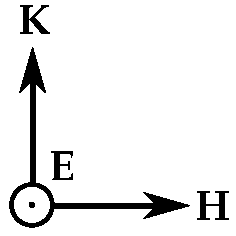
\includegraphics[width=.12\textwidth]{img/tripletKEH.pdf}}
	\end{overpic}
	\begin{overpic}[width=.48\textwidth]{img/Slab_eps012_d15.pdf}   \put(1,96) {\textbf{(b)}} \end{overpic}
\end{figure}
%}}}
\begin{figure}[ht] %{{{ fg_Slab_fillfraction015_epsilon_comparison
	\caption{Amplitude of \textbf{(a)} reflectance, \textbf{(b)} transmittance and \textbf{(c)} effective index of refraction $\Neff$ (real part solid, imaginary part dashed) for the dielectric slab of 15\% fill fraction in a 300 $\upmu$m unit cell, and varied permittivity of the dielectric $\epsrl \in \{4,12,20\}$} \label{fg_Slab_fillfraction015_epsilon_comparison} \centering \vspace{-3mm}
\begin{tabular}{r}
\begin{overpic}[width=0.95\textwidth]{img-meep/Slab_fillfraction015_epsilon_comparison_r.pdf} \put (-1,27) {\textbf{(a)}} \end{overpic}\vspace{-0.055\textwidth}\\
\begin{overpic}[width=0.95\textwidth]{img-meep/Slab_fillfraction015_epsilon_comparison_t.pdf} \put (-1,27) {\textbf{(b)}} \end{overpic}\vspace{-0.055\textwidth}\\
\begin{overpic}[width=0.96\textwidth]{img-meep/Slab_fillfraction015_epsilon_comparison_n.pdf} \put (-1,37) {\textbf{(c)}} \end{overpic}\vspace{-0.\textwidth}\\
\end{tabular}
\end{figure}
%}}}
\paragraph{Characteristics of Bragg-type band gaps}%{{{
The lower and upper edge of the photonic bands are located the high-symmetry points of the Brillouin zone, such as $\mathbf{\Gamma}$ or $\mathbf{X}$, which are equivalent to the wavenumber $K=m\pi/a$ for $m\in\mathbb{Z}$ in the one-dimensional case discussed. Whenever $K$ is in one of these points, the electric and magnetic fields are periodic in space, and can be easily visualized. The side plots of \ref{fg_1dbd} show the shapes of the electric field $E_x$ in the $(y,z)$ plane at respective frequencies of the band edges. To stress the fact that the field is periodic even in the $\mathbf{X}$ point, each of the side plots spans over 2$\times$2 unit cells. 

An important characteristic of each field pattern is the set of all points where the field amplitude remains zero over the evolution of time. Such sets will be denoted as \textit{nodal planes}, or also, more accurately, \textit{nodal surfaces}.

From all pairs of field plots that are connected by a photonic band (i.e. X2-$\Gamma2$, $\Gamma3$-X3 etc.), it can be deduced that one nodal plane dividing the unit cell in perpendicular orientation to the wave vector is always added when the frequency increases from the lower band edge to the upper one. This rule is more general and is satisfied by other structures, too. 

Typical for all Bragg band gaps (i.e. X1-X2, $\Gamma2$-$\Gamma3$, etc. in \ref{fg_1dbd}) is that between the lower and upper edges of each band gap, the phase increase across an unit cell does not change and thus $K$ remains constant, as does the number of the nodal planes. The field does change between these points, however, and the change is in the location of the \textit{nodal planes} such that the upper band-gap edge concentrates the field energy in mostly lower-permittivity regions. 

%}}}
\paragraph{Bragg and Fabry-Pérot resonances} %{{{
The \textit{Bragg condition} for the formation of a band gap in a periodic structure is that an integer number of half waves fits into the unit cell; i.e. that the phase difference $\phi_{1+2}$ of the wave along the unit cell is 
\begin{equation} \phi_{1+2} = d_1 n_1 \frac{\omega}{c} + d_2 n_2 \frac{\omega}{c} = \pi m, \text{ where } m\in \mathbb{Z}. \label{eq_braggcond}\end{equation}
where $d_{1,2}$ are the thicknesses and $n_{1,2}$ are the refractive indices of the two layers.

\begin{figure}[t] \caption{\textbf{(a)} Reflectance and \textbf{(b)} the imaginary part of the retrieved refractive index for a 1-D PhC, with filling fraction of 15~\% in a 300~$\mu$m unit cell, as a function of frequency and dielectric permittivity. On the right panel, the Fabry-Pérot condition from Eq. (\ref{eq_fpcond}) are marked by a thin dash-dotted line.} \label{fg_slab_eps_scan} \centering 
\begin{overpic}[width=0.48\textwidth]{img-meep/Slab_fillfraction015_epsilon_scan_r.pdf}\put(-1,80){\textbf{(a)}}\end{overpic}
\begin{overpic}[width=0.48\textwidth]{img-meep/Slab_fillfraction015_epsilon_scan_ni.pdf}\put(-1,80){\textbf{(b)}}\end{overpic}
\end{figure}

\begin{figure}[t] \caption{\textbf{(a)} Reflectance and \textbf{(b)} the imaginary part of the retrieved refractive index for a 1-D PhC, with relative dielectric permittivity of 4, as a function of frequency and filling fraction in a 300~$\mu$m unit cell} \label{fg_slab_ff_scan} \centering 
\begin{overpic}[width=0.48\textwidth]{img-meep/Slab_epsilon4_fillfraction_scan_r.pdf}\put(-1,80){\textbf{(a)}}\end{overpic} 
\begin{overpic}[width=0.48\textwidth]{img-meep/Slab_epsilon4_fillfraction_scan_ni.pdf}\put(-1,80){\textbf{(b)}}\end{overpic}
\end{figure}

The width of the band gap grows with the amplitude of the wave scattered from the unit cell. This amplitude however also depends on frequency and, in the case of a lossless dielectric slab, it vanishes whenever an integer number of the half-waves fits into either of the dielectric layers. For comparison with Eq. (\ref{eq_braggcond}), this condition is
\begin{equation} \phi_{1} = d_1 n_1 \frac{\omega}{c} = \pi m \text{\quad or \quad} \phi_{2} = d_2 n_2 \frac{\omega}{c} = \pi m, \text{ where } m\in \mathbb{Z}. \label{eq_fpcond}\end{equation}
Note that unlike the Bragg resonance, this effect can be observed even in a single isolated unit cell; in fact it is the well known \textit{Fabry-Pérot resonance}. 

The vicinity of a Fabry-Pérot resonance influences the position and width the neighbouring band gap, which can be found for different dielectric permittivity of the slab $\epsrl\in\{4,12,20\}$ in Fig. \ref{fg_Slab_fillfraction015_epsilon_comparison}.

As special case, the conditions for both Bragg and Fabry-Pérot resonances can be fulfilled simultaneously: a \textit{zero-width band gap} results and two photonic bands are adjacent to each other in the same way as they were in vacuum (c. f. Fig. \ref{fg_1dbd}a). In all cases of zero-width PBGs, the dispersion curves appear to approach the boundary of photonic bands (located in a high-symmetry point in the Brillouin zone) as lines with nonzero slope. In the analogy with the dispersion of electrons in a solid, this can be viewed as a \textit{Dirac point for photons-polaritons}, where the photons-polaritons have zero effective mass. The corresponding isofrequency contour may have a cusp in this point, rendering invalid even the generalised notion of the refractive index as elaborated in Section \ref{indexofrefraction}.

An example of a structure that exhibits multiple zero-width band gaps is the 1-D PhC with equal optical thickness of both slabs ($d_1 n_1 = d_2 n_2$), but multiple such points exist when the dielectric permittivity or the dielectric filling fraction is changed, as depicted in Figs. \ref{fg_slab_eps_scan} and \ref{fg_slab_ff_scan}, respectively. These plots are also the simplest examples of the interplay between the individual resonance contained in the dielectric structure and the overall band-gap structure, a topic that will be discussed later in more detail.

%}}}
\paragraph{Local effective parameters of a 1-D PhC}%{{{
Employing the \textit{s-parameter} method based on FDTD simulation, as described in Chapter \ref{chapter_sparam}, one can obtain the scattering parameters (i.e. complex reflectance and transmittance) of a finite layer of the periodic structure, and eventually retrieve its local effective parameters: the index of refraction $\Neff(f)$, impedance $\Zeff(f)$, permittivity $\eeff(f)$ and permeability $\meff(f)$. The first one is plotted in Fig. \ref{fg_Slab_fillfraction015_epsilon_comparison}c, allowing to clearly identify the Bragg band gaps as regions where $\Neff'$ follows one of the Brillouin zone boundaries and $\Neff'' < 0$.

The question is to what extent the three remaining local parameters, $\Zeff$, $\eeff$ and $\meff$, have any physical meaning. As a generally accepted approach, they will be considered meaningful only for the long wavelength limit, i.e. $K$ close to the $\mathbb{\Gamma}$ where the effects of the spatial dispersion should be negligible. According to Fig. \ref{fg_Slab_fillfraction015_epsilon_comparison}c, this is for frequencies up to 100 or 200 GHz only. At any higher frequency, the retrieved wavenumber $K$ approaches the Brillouin zone boundary, marked by the thin dash-dotted line, and grows further.

In the low frequency limit of 1-D PhC, it was always observed that
\begin{enumerate}
\item{$\Zeff \approx 1/\Neff$, thus the effective permeability is $\meff = \sqrt{\Neff\Zeff} \approx 1$.} 
\item{The effective permittivity $\eeff$ is the weighted average of the constituent media, which determines the low-frequency limit for the refractive index:
	\begin{equation} \left.\Neff\right|_{K\ll 2\pi/a} =\left. \sqrt{\eeff}\right|_{K\ll 2\pi/a} \approx \sqrt{\frac{d_1 n_1^{2} + d_2 n_2^{2}}{d_1+d_2}} \label{eq_phc_eeff}\end{equation}
	}
\end{enumerate}
Notice in Fig. \ref{fg_Slab_fillfraction015_epsilon_comparison}c that $\Neff$ at higher frequencies converges towards its asymptotic value $\left.\Neff\right|_{K\rightarrow +\infty}$, which differs from the value obtained by Eq. (\ref{eq_phc_eeff}):
\begin{equation} \left.\Neff\right|_{K\rightarrow +\infty} \approx \frac{d_1 n_1 + d_2 n_2}{d_1+d_2} \label{eq_phc_neff}\end{equation}
The difference comes from that in the low-frequency limit, the electromagnetic energy concentration is higher in the areas of higher permittivity, whereas in the high-frequency limit it appears to be distributed evenly.
Note that with the correct branch retrieval procedure, the index of refraction never drops with frequency except for the photonic band gaps. Negative derivative of $\Neff(f)$ would otherwise imply that the group velocity would be higher than the phase velocity \cite{mikki2009electromagnetic}, which was never observed in 1-D PhC.

% TODO \paragraph{Transmission through a finite number of unit cells}
% illustrate the band-gap formation \cite{laktionov2008}
% (todo) find python script ----> compare TMM and FDTD for metallic slabs
% note the ripples inside the band-gap (for more cells)
% and note that the NRW effective parameters do not change; the method is exact here due to absence of evanescent fields, whose detrimental effect was described in -todo-
% finite planar structure with defect mode \cite{skoromets2013}
%\begin{figure} \caption{1red.pdf}  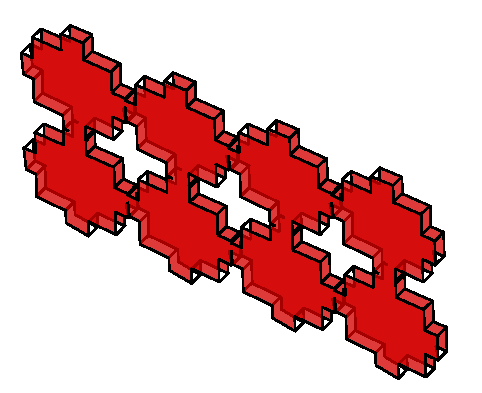
\includegraphics[width=3cm]{img/multilay_1red.pdf}
               %\caption{2gn.pdf}   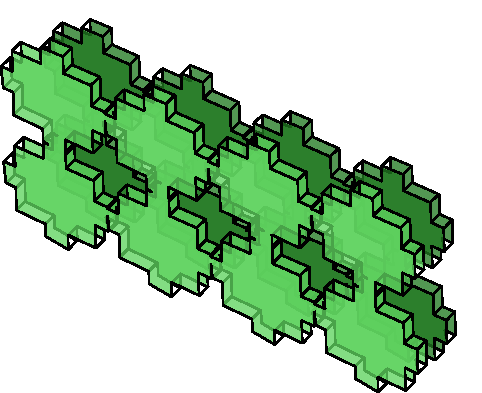
\includegraphics[width=3cm]{img/multilay_2gn.pdf}
               %\caption{3bu.pdf}   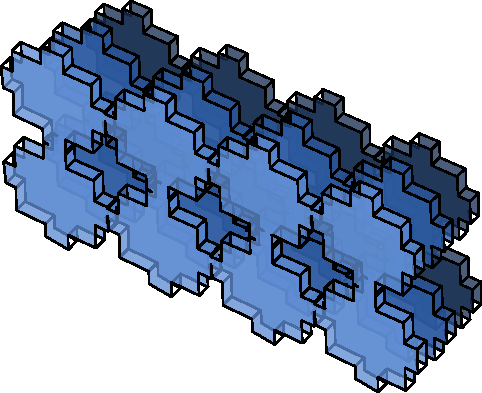
\includegraphics[width=3cm]{img/multilay_3bu.pdf}
               %\caption{3grey.pdf} 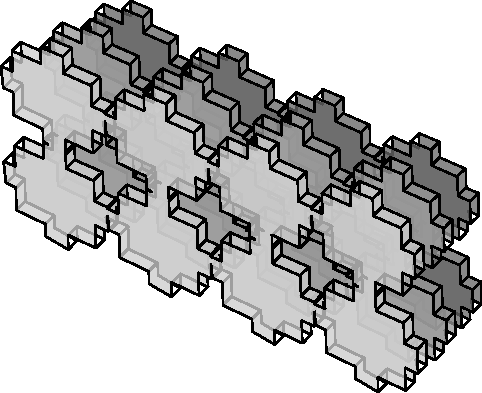
\includegraphics[width=3cm]{img/multilay_3grey.pdf}
               %\caption{4vio.pdf}  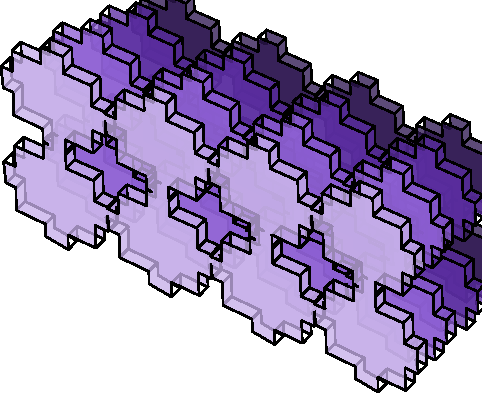
\includegraphics[width=3cm]{img/multilay_4vio.pdf} \end{figure} 

%}}}
\FloatBarrier %====================================================================================================
%}}}
\section{Wire medium} \label{chap_wiremedium}%{{{
\paragraph{High-frequency behaviour}%{{{
The structure formed of a regular square lattice of conductive wires exhibits more interesting properties when the electric field is parallel to the wires, and this polarisation will be assumed in the following. The lattice of wires perpendicular to the electric field does not appreciably interact with the electromagnetic wave, until the wire width is of similar magnitude to their spacing; such a case is discussed in Section \ref{section_eot}.

In the high-frequency part of the spectrum above the first photonic band, where more than a half wave fits into the unit cell, the layers of metallic rods can be approximated by thin scattering slabs from the previous section, since the high-frequency interaction of the wave can be described of photonic bands alternating with Bragg band gaps. In contrast with the dielectric PhC described above, no Fabry-Pérot resonances are observed and the scattering strength of the wire layers reduces monotonously with growing frequency.

\begin{figure}[ht] \caption{Amplitude of \textbf{(a)}  reflectance, \textbf{(b)} transmittance \textbf{(c)} effective index of refraction $\Neff$ and \textbf{(d)} effective permittivity $\eeff$ for the array of wires made of gold, depending on the wire radius $\rho_w \in \{1, 2, 4, 8, 16\}$ $\mu$m with a fixed unit cell size $a = 100$ $\mu$m and grid resolution of 1 $\mu$m. } \label{fg_Slab_fillfraction015_wireradius_scan} \centering \vspace{-3mm}
\begin{tabular}{r}
\begin{overpic}[width=0.85\textwidth]{img-meep/Wires_wireradiusscan_r.pdf} \put (-1,28) {\textbf{(a)}} \end{overpic}\vspace{-0.060\textwidth}\\ 
\begin{overpic}[width=0.85\textwidth]{img-meep/Wires_wireradiusscan_t.pdf} \put (-1,28) {\textbf{(b)}} \end{overpic}\vspace{-0.057\textwidth}\\
\begin{overpic}[width=0.86\textwidth]{img-meep/Wires_wireradiusscan_n.pdf} \put (-1,28) {\textbf{(c)}} \end{overpic}\vspace{-0.055\textwidth}\\
\begin{overpic}[width=0.86\textwidth]{img-meep/Wires_wireradiusscan_eps.pdf} \put (-1,28) {\textbf{(d)}} \end{overpic}\vspace{-0.030\textwidth}\\
\end{tabular}
\end{figure}

%}}}
\paragraph{Inductive behaviour at low frequencies}%{{{
At low frequencies, in contrast, the interaction of the conductive wires with the electromagnetic wave becomes very strong and leads to completely different behaviour than that described above. For a frequency range from zero up to the \textit{effective plasma frequency} $f_p$, the array exhibits a band gap where $\Neff$ is pure imaginary and $k'\approx 0$. Therefore, in the low-frequency part of the spectrum, the local effective permittivity $\eeff$ is a physically meaningful quantity and follows the law typical of inductive media:
\begin{equation} \eeff(f) = 1 - \frac{f^{2}}{f_p^{2}}\label{eq_eeff_plasma}\end{equation}
Such a dependence of $\epsrl$ was already used in the Drude model in Eq. (\ref{eq_drude_eps}), and plotted in Fig. \ref{fg_Au_models}. Owing to this similarity to metals or plasma, wire arrays are denoted also as \textit{diluted metal} or \textit{artificial plasma} since 1950s \cite{merkel1973simulation, rotman1962plasma}, or as \textit{metallic delay dielectrics}, owing to the possibility to manipulate the phase and group velocities  \cite[p. 54]{brown1953artificial}.

The physical origin of $\eeff<0$ is different than in continuous media, where it is \textit{kinetic}, i.e., due to the effective mass of electrons. In contrast, the negative effective permittivity in wire arrays is the result of the \textit{self inductance} due to the magnetic field circulating around the conductor. 

Except for optical frequencies, $f_p$ does not substantially depend on the internal plasma frequency of the constituent metal, and such behaviour can be obtained even if wires are thought to be made of a perfect electric conductor (PEC).
The plasma frequency does, however, depend on the geometry described by two parameters, the wire radius $\rho_w$ and the unit cell size $a$. 

%}}}
\paragraph{Behaviour close to the effective plasma frequency}%{{{
The dependence of $f_p$ on the wire radius $\rho_w \in \{1, 2, 4, 8, 16\}$ $\upmu$m is illustrated by the spectra of reflectance, transmittance, refractive index and effective permittivity in Fig. \ref{fg_Slab_fillfraction015_wireradius_scan}. The effective plasma frequency $f_p$ can be easily determined as the point where $\eeff'(f)$ crosses zero  in the plot \ref{fg_Slab_fillfraction015_wireradius_scan}d. This coincides with the lower edge of the first photonic band in Fig. \ref{fg_Slab_fillfraction015_wireradius_scan}c. 

For the limit $f \rightarrow f_p+$, the \textit{phase velocity} $$c/n = c/\sqrt{\eeff(f)}$$ is proportional to $(f-f_p)^{-1/2}$ and thus very high. Conversely, the \textit{group velocity} $$v_g \approx 2\pi \mathrm{d}f/\mathrm{d}k = \mathrm{d}f/\mathrm{d}n$$ vanishes, being proportional to $(f-f_p)^{+1/2}$. Hence the product of the phase and group velocities close to $f_p$ remains nearly constant $c^2$, which is a phenomenon commonly encountered also near the \textit{cut-off frequency} of metallic waveguides.

Exactly at $f=f_p$, the wire array medium can support the longitudinal oscillations of the charge, oriented parallel to the wires. They bear a close resemblance to plasmons in bulk media \cite{pendry1996extremely}.

Notice that for a single cell, the transition from negative to positive permittivity is not accompanied by any obvious spectral feature on the reflection/transmission plot. Except for the zero frequency, a layer of wires has always nonzero transmittance that increases with frequency. Independent of the wire conductivity, it is not possible to build a 100\% efficient wire polarizer.

%}}}
\begin{figure}[th]%{{{ fg_omegap_a
  \begin{minipage}[c]{0.69\textwidth}
\begin{overpic}[width=.98\textwidth]{img/EWire_plasmaF_spacingscan.pdf} \put (-1,60) {\textbf{(a)}} \end{overpic}\\
\begin{overpic}[width=\textwidth]{img/EWire_plasmaF_radiusscan.pdf}  \put (-1,58) {\textbf{(b)}} \end{overpic}\\
  \end{minipage}
  \begin{minipage}[c]{0.3\textwidth}
	  \caption{Comparison of numerical results (dots) and two analytic models (solid and dotted lines) for plasma frequency $f_p$ of a wire medium: \textbf{(a)} $f_p$ as a function of wire spacing for two different wire radii of 16 $\mu$m and 8 $\mu$m (red and blue curves/dots, respectively). The empty symbols correspond to significantly reduced FDTD resolution, added for comparison. \textbf{(b)} $f_p$ as a function of wire radius $\rho_w$.}\vfill \label{fg_omegap_a}
  \end{minipage}  
\end{figure} 

%}}}
\paragraph{Plasma frequency as a function of wire radius and unit cell size}%{{{
From Fig.  \ref{fg_Slab_fillfraction015_wireradius_scan}, it can be also deduced that $f_p$ is approximately proportional to the logarithm of $\rho_w$ if $\rho_w \ll a$. This is related to that a thicker wire should have slightly lower inductance per unit length (sometimes denoted as its \textit{self-inductance}). 

The effect of wire spacing $a$ is the opposite; with $a$ growing, the magnetic field has more space to circulate around the wir and $f_p$ reduces. 

Different analytic models were proposed for description of both effects. The early model by Pendry \textit{et al.} from 1996 \cite{pendry1996extremely} works well for thin wires: 
\begin{equation} f_p(\rho_w,a) \approx \sqrt{\frac{c^2}{2\pi \, a^2 \, \ln(\frac{a}{\rho_w})}}. \label{eq_fp_pendry}\end{equation}
Its refinement by Maslovski \textit{et al.} from 2003 \cite{maslovski2002wire} should be valid also for wires with relatively high fill fraction:
\begin{equation} f_p(\rho_w,a) \approx \sqrt{\frac{c^2}{2\pi \, a^2 \, \ln\left(\frac{a^2}{4\rho_w (a-\rho_w)}\right)}} \label{eq_fp_maslovski}\end{equation}

We ran two series of wire array simulations as a simple verification of both the FDTD algorithm against the mentioned analytic models. In the first series plotted in Fig. \ref{fg_omegap_a}a, we kept the wire radius constant $\rho_w = 16\,\upmu$m, or and changed the wire spacing $a$ (red points). We changed the radius to $\rho_w = 8\,\upmu$m in the second batch, marked by blue points. For comparison, we plot in the plasma frequency predicted by both analytic models from Eqs. (\ref{eq_fp_maslovski}, \ref{eq_fp_pendry}) as full and dotted lines with the color corresponding to the simulation parameters, respectively. 

To test the possible error introduced by the FDTD algorithm, we ran the simulation with different resolution - results with fine $1$ $\upmu$m grid are denoted by full circles, results with coarse $4$ $\upmu$m grid with empty squares overlaid relatively close to the respective high-resolution results.

In the second series of simulations plotted in Fig.  \ref{fg_omegap_a}b, we kept the spacing $a = 100$ $\upmu$m and changed the wire radius $r$. The analytic model and FDTD simulation give similar results (up to 5 \%) even for wire radii approaching roughly $a/4$. For thicker wires, the analytic model predicts higher plasma frequency than FDTD.  To conclude, the results of the model presented by Maslovski match the FDTD simulation with good accuracy for thin wires (where $r \lesssim a/5$). One possible application of the wire medium is in the construction of negative refractive index metamaterials, where a small negative real value of effective permittivity is desired.%%todo rewrite?

%}}}
%TODO \paragraph{Oblique propagation of the wave} % {{{
%ref Homogenisation of nonlocal media such as wires 
%\cite{capolino2009book}
%\cite{silveirinha2007metamaterial}
%\cite{belov2003strong}
%\cite{belov2002dispersion}
%\cite{silveirinha2005homogenization}
% nice refs  from 1950-1970: http://ece-research.unm.edu/summa/notes/SSN/note192.pdf

%}}}
\FloatBarrier %====================================================================================================
%}}}
\section{Cut wires} \label{section_cutwires}%{{{
\paragraph{Individual resonances}%{{{
The low-frequency behaviour of the wire array is determined by the distributed inductance of the wires, which introduces negative effective permittivity up to the plasma frequency $f_p$. When the wires are cut in each unit cell, a three-dimensional periodic lattice of antennas is formed. Its important parameters are not only the inductance along each antenna, but also the capacitance across the gap between wires. In an analogy with a series LC (coil-capacitor) circuit, such antennas exhibit \textit{individual resonances} at some nonzero resonant frequency $0<f_r<f_p$. 

These resonances couple to the electromagnetic field by means of their electric dipole, so they are denoted shortly as \textit{electric resonances}. This does not mean that no magnetic field is involved; in fact, the energy is exchanged between the resonant electric and magnetic fields each quarter-period. The situation partially changes with decreasing size of the particles. At optical frequencies, the energy is exchanged between the electric field and the kinetic energy of the electrons, while the magnetic field circulating around the metallic particle plays a minor role only. Such regime is known as \textit{plasmonic resonances} and was described by Mie in 1908 \cite{mie1908beitrage}.
% note the Bohren and Huffman implementation is in /home/filip/PhD/Misc/120400_analytic_Mie_scattering/

The spectra for the cut-wire structure are depicted in Fig. \ref{fg_CutWires_wireradius1u_cutwidth_comparison} for different cut distances $d_c$. Starting with the thinnest wire of $\rho_w = 2$ $\upmu$m (red curve), we can identify the individual resonance as the point close to  1200 GHz where even a single layer of unit cells reflects full wave amplitude and the transmittance drops to zero. Towards higher or lower frequencies from the resonance, the transmittance is relatively high.

%% TODO check if the spatial dispersion would be visible in the CDH plots
%% ...even here, with particles infinitesimally thin along the wave-vector, the spatial dispersion may be significant; arguably it was observed in 1970s by Merkel \cite{merkel1973simulation}, who remarks that
%% "It is interesting that the more exact expressions for the dielectric constant of the artificial dielectric, which considered both the effect of the capacitive dipole impedance and the dipole-dipole interaction, did not model the behavior of a Lorentzian plasma as well as the original simplified approach"
%% TODO note about plasmonic particles 
%}}}
\begin{figure}[h!] \caption{Amplitude of \textbf{(a)} reflectance, \textbf{(b)} transmittance, \textbf{(c)} effective index of refraction $\Neff = \Neff' + \ii \Neff''$ for the array of cut wires of radius $r_w = 1$ $\upmu$m made of gold, depending on cut distance $r_w\in \{2, 4, 8, 16, 32, 64\}$ $\upmu$m. The unit cell is cubic and its size is $a=100$ $\upmu$m.\\%{{{
In plot  \textbf{(d)}, the effective permittivity is illustrated for the thinnest cut distance $d_c = 2$ $\upmu$m. Although retrieved for the entire spectrum, the local effective parameters have physical meaning only when the wavelength is much larger than $a$, i.e. roughly from 0 to 500 GHz and from 1220 to 1280 GHz.} \label{fg_CutWires_wireradius1u_cutwidth_comparison} \centering \vspace{-3mm}
\begin{tabular}{r}
\begin{overpic}[width=0.85\textwidth]{img-meep/CutWires_wireradius1u_cutwidth_comparison_r.pdf} \put (-1,28) {\textbf{(a)}} \end{overpic}\vspace{-0.059\textwidth}\\
\begin{overpic}[width=0.85\textwidth]{img-meep/CutWires_wireradius1u_cutwidth_comparison_t.pdf} \put (-1,28) {\textbf{(b)}} \end{overpic}\vspace{-0.056\textwidth}\\
\begin{overpic}[width=0.86\textwidth]{img-meep/CutWires_wireradius1u_cutwidth_comparison_n.pdf}\put (-1,28) {\textbf{(c)}} \end{overpic}\vspace{-0.056\textwidth}\\
\begin{overpic}[width=0.85\textwidth]{img-meep/CutWires_wireradius1u_cutwidth_comparison_eps_r2.pdf} \put (-1,28) {\textbf{(d)}} \end{overpic}\vspace{-0.030\textwidth}\\
%\begin{overpic}[width=0.85\textwidth]{img-meep/CutWires_wireradius1u_cutwidth_comparison_ni.pdf}\put (-1,28) {\textbf{(d)}} \end{overpic}\vspace{-9.5mm}\\ \begin{overpic}[width=0.85\textwidth]{img-meep/CutWires_wireradius1u_cutwidth_comparison_eps_r2.pdf}\put (-1,28) {\textbf{(d)}} \end{overpic}\vspace{-0.030\textwidth}\\
\end{tabular}
\end{figure}
%}}}
\paragraph{Dispersion near an individual resonance}%{{{
Each individual resonance in a periodic structure forms a characteristic shape in the spectrum of effective index of refraction $\Neff(f)$. The following description will therefore be applicable to individual resonances in other resonant structures, as well. 

\begin{enumerate}
\item{At frequencies under the resonance, the electric dipole of the antenna oscillates in phase with the driving field and the resonance contributes the effective index of refraction $\Neff'(f)$. 
The spectrum of a periodic structure with an individual resonance differs from the spectrum of a homogeneous medium that was already described at the Lorentzian resonance curve in Fig. \ref{fg_oscillator_spectrum}b.
At some frequency $f \lesssim f_r$ below the resonance, the index of refraction $\Neff'(f)$ becomes high enough to join the closest Brillouin zone boundary which was above it. From this point up to the resonance frequency $f_r$, $\Neff(f)$ has nonzero imaginary part, and the medium exhibits a band gap.
} 
\item{Exactly at the resonance frequency, the interaction of the dipole with the field changes its sign, since above the resonance, the dipole starts to be oriented opposite to the driving field. 
The real part of the refractive index $\Neff'(f)$ ceases to follow one Brillouin zone and transitions to another Brillouin zone below it. In local media, individual resonances appears to be the only occasions for $\Neff'(f)$ to transition downwards.

The imaginary part of the refractive index, $\Neff''(f)$, is required by the Kramers-Kronig relations to exhibit a sharp peak at the resonance frequency, which is superposed over the broader background stemming from the band gap (see Fig. \ref{fg_CutWires_wireradius1u_cutwidth_comparison}c). 

The spectral width of the transition and peak is inversely proportional to the quality of the resonance. Whenever the structure is built from realistic materials with nonzero losses and its spatial dispersion can be neglected, $\Neff(f)$ is a continuous complex function.
} 
\item{The band gap continues up to some frequency $f > f_r$, where another photonic band begins between the same pair of Brillouin zones.  
} 
\end{enumerate}

The most important observation is that the resonance curve of $\Neff(f)$ in periodic structures is constrained between the closest two Brillouin zone boundaries, which can be understood as the "floor" and "ceiling" for the dispersion curve. Apparently a single individual resonance can not shift the transmittance phase by more than $\pi$ per each layer of unit cells. It can therefore introduce a band of imaginary $\Neff$, but for $\Neff$ to reach negative values, two resonances must be combined.

The impact of the individual resonances on the effective parameters $\eeff(f)$ and $\meff(f)$ will be discussed in the later section focused on the dielectric resonators. % TODO verify that I have done this

%}}}
\paragraph{Effects of the cut distance $d_c$}%{{{
An increase of the cut distance $d_c$ clearly increases the resonance frequency $f_c$. The reason is twofold: for a cut width small relative to the unit cell size, $d_c\ll a$, it is mostly due to reduced capacitive coupling between the cut wires; for cut width comparable or greater than the unit cell size, $d_c \gtrsim a$, reduction of the cut-wire inductance is more important.

Both the individual and Bragg-type resonances can be identified in the plot for different $d_c$ in Fig. \ref{fg_CutWires_wireradius1u_cutwidth_comparison}c. When $d_c \sim 16$  $\upmu$m, the individual resonance shifts above 1.5 THz and exchanges its order with the Bragg band gap. 
For $d_c \gtrsim 32$  $\upmu$m on, the individual resonances are similar to those for a $d_c\sim 2$ $\upmu$m, but are shifted by one Brillouin zone up.

%}}}
\begin{figure}[h!] \caption{Amplitude of \textbf{(a)} reflectance, \textbf{(b)} transmittance and \textbf{(c)} effective index of refraction $\Neff = \Neff' + \ii \Neff''$ for a metamaterial made of cut wires with radius $r_w$. Cut distance $d_c = 2$ $\mu$m, unit cell size $a=100$ $\mu$m.} \label{fg_CutWires_wirecut2um_wireradiusscan} \centering \vspace{-3mm} %{{{
\begin{tabular}{r}
\begin{overpic}[width=0.85\textwidth]{img-meep/CutWires_wirecut2um_wireradiusscan_r.pdf} \put (-1,28) {\textbf{(a)}} \end{overpic}\vspace{-0.060\textwidth}\\
\begin{overpic}[width=0.85\textwidth]{img-meep/CutWires_wirecut2um_wireradiusscan_t.pdf} \put (-1,28) {\textbf{(b)}} \end{overpic}\vspace{-0.060\textwidth}\\
\begin{overpic}[width=0.85\textwidth]{img-meep/CutWires_wirecut2um_wireradiusscan_n.pdf}\put (-1,28) {\textbf{(c)}} \end{overpic}\vspace{-0.030\textwidth}\\
\end{tabular}
\end{figure}
%}}}
\paragraph{Effects of the wire radius $\rho_w$}%{{{
The dependence of the resonance frequency $f_c$ on the wire radius, Fig. \ref{fg_CutWires_wirecut2um_wireradiusscan}, is somewhat more complicated: For thin enough wires in the $a=100$ $\upmu$m unit cell, the resonance frequency decreases with growing $\rho_w$, since the inter-wire capacity increases. 
For high enough $\rho_w$ an opposite mechanism prevails; $f_c(\rho_w)$ then starts growing as a result of reduction of the wire inductance.

While the change of the cut-wire radius $\rho_w$ relatively weakly reflects in the resonance frequency, its major impact is in the \textit{strength} of the individual resonance. Thick wires lead to stronger reflection out of resonances, which also translates into a wider band gap in Fig. \ref{fg_CutWires_wirecut2um_wireradiusscan}c.

%}}}
\paragraph{Experimental measurement of cut wire spectra}%{{{ 
Although we did not fabricate any cut-wire metamaterial, we used the terahertz time-domain spectroscopy to characterise cut-wire-on-silicon structures, one representative of which is photographed and sketched in Fig. \ref{fg_bousek}. The metallic wires were deposited on a silicon substrate, and at their ends, the silicon was doped to form diode-like transitions. 
\begin{figure}[ht] \caption{The sample of cut wires (pale yellow) on silicon (cyan) substrate. \textbf{(a)} Natural-colour photograph from an optical microscope,  \textbf{(b)} Geometry of the wires in micrometers. They were measured to be $6.5$ $\mu$m wide and $30$ $\mu$m long. The periodicity of cut-wires was $30\times 50$ $\mu$m.  } \label{fg_bousek} \centering 
\begin{overpic}[height=.40\textwidth]{img/bousek_splitwires_microphoto.pdf}  \put(0,78) {\textbf{(a)}} \end{overpic}\quad
\begin{overpic}[height=.40\textwidth]{img/bousek_splitwires_drawing.pdf}  \put(0,95) {\textbf{(b)}} 
		\put(55,0){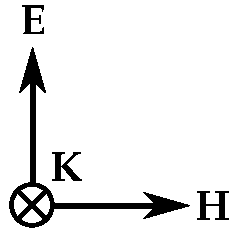
\includegraphics[width=.12\textwidth]{img/tripletEKH.pdf}} % todo
\end{overpic}
\end{figure}

This kind of structure was designed to operate as a switch for the terahertz radiation, controlled by the current flowing along the orientation of the wires and modulating the conductivity of semiconductor transitions at the ends of each cut wire. For an unknown reason, the modulation of the terahertz signal was very weak, if any, in all of 7 supplied samples. The only observed kind of systematic modulation manifested as 2.2\% drop in amplitude of the transmitted terahertz waveform, and its temporal advance by no more than 18 fs. These values required to feed the structure with a maximum modulation signal, dissipating roughly 10 watt peak thermal power.

The sample presented above in Fig. \ref{fg_bousek}, though not applicable as a modulator, exhibits a clear electric resonance around 1550 GHz. This resonance is substantially broadened and weakened by the losses of the structure (red line in Fig. \ref{fg_bousekspectra}). A FDTD simulation of thin metallic stripes 30 $\upmu$m long and 6.5 $\upmu$m wide on a silicon substrate did not match the experimental spectra very well (green line in Fig. \ref{fg_bousekspectra}). 
%}}}
\begin{figure}[ht]  % fg_bousekspectra%{{{
	\caption{Comparison of experimental (red line) and simulated spectra (green and blue lines) for the cut-wire on silicon structure. The green line corresponds to the original geometry from Fig. \ref{fg_bousek}b; a better match with the experiment is obtained by changing the length of stripes from 30 to 40 $\mu$m (blue line).} \label{fg_bousekspectra} \centering 
\begin{overpic}[width=.85\textwidth]{img-expe/bousek.pdf}\end{overpic}
\end{figure}
Much better match was obtained by simple elongation of the conductive stripes to 40 $\upmu$m (blue line in Fig. \ref{fg_bousekspectra}). This may reflect the fact that the wires were surrounded by a highly doped, conductive zones of silicon.
Although not taking into account the dissipative losses, such a simulation correctly identifies the resonance freqeuncy of the stripes. It also, at least quantitatively, matches the asymmetric spectral shape, which is caused by the onset of diffraction into the silicon substrate at $f_c = c/(50\;$ $\upmu$m$)/N_{\text{Si}} \approx 1730$ GHz. 

The presented simulations were not optimized for the dissipative losses in silicon, which could be modeled with more detailed knowledge of the structure preparation. %TODO unduplicate rewrite?

%}}}
%     \FloatBarrier %====================================================================================================
%     \section{Electric resonators} \label{section_esrr} % note about plasmonic particles 
%     OFF \paragraph{Comparison of spectra to the cut wires}%{{{
%     From Figs. \ref{fg_CutWires_wirecut2um_wireradiusscan} and \ref{fg_CutWires_wireradius1u_cutwidth_comparison} it follows that for any practically attainable geometry, the frequency of the first individual resonance in cut-wire arrays is always relatively close to the first Bragg band gap. 
%     
%     A viable way to shift the resonance frequency much lower, without changing the unit cell size nor resorting to submicrometre cut distances, is to replace straight wire antennas by \textit{electric split-ring resonators}, % TODO cite 
%     depicted in Fig. \ref{fg_eSRR}.
%}}}
\FloatBarrier %====================================================================================================
%}}}
\section{Split-ring resonator} \label{section_srr} % %{{{
\paragraph{Resonances with magnetic dipole moment}%{{{
The fundamental resonance in a cut wire has the electric dipole moment only. The resonant magnetic field circulates around the wire and due to its rotational symmetry along the $x$-axis, the magnetic dipole moment is zero. Other structures can support resonances of lower symmetry with regards to the $x$-axis, thus having a magnetic dipole moment.

One of the simplest examples is formed by bending the wire into a "C"-shaped \textit{split-ring resonator} (SRR). To reduce the resonant frequency, capacitor pads can be added to the cut, as shown in Fig. \ref{fg_SRR_types}a. The first resonance in its spectrum has a dominant magnetic dipole moment, and will be denoted simply as the \textit{magnetic resonance}. The electric current flows through the wire along a circular path, while the magnetic field has a toroidal shape around the wire.   

The very concept of SRR is at least as old as the Hertz's experiments with the spark-gap transmitter from 1880s.
As described in the historical review of Ref. \cite[pp. 120--126]{solymar2009waves}, first SRR arrays were built in early 1980s with the aim to build an effective medium with highly lossy complex permeability; a decade later asymmetric SRRs were used to achieve strong bianisotropy. Many publications cite Refs. \cite{pendry1999magnetism,pendry2000negative} from Pendry et al. as the first application of SRR array for achieving negative effective permeability and index of refraction, respectively. Since then, the number of SRR-related publications has grown rapidly. 
\label{negn_srr}

\begin{figure}[h] \caption{Variants of the split-ring resonators, viewed from the side perpendicular to the magnetic field: \textbf{(a)} classical SRR, \textbf{(b)} symmetric SRR with two splits, \textbf{(c)} one of the designs of an electric SRRs having a central bar, \textbf{(d)} a similar structure where the central bar was split by a capacitor with pad radius $\rho_c$, allowing to tune the electric resonance} \label{fg_SRR_types} \centering 
\begin{overpic}[height=0.25\textwidth]{img/drawing_SRRpad.pdf}\put (1,80) {\textbf{(a)}}\end{overpic}\qquad
\begin{overpic}[height=0.25\textwidth]{img/drawing_sSRRpad.pdf}\put (-2,80) {\textbf{(b)}}
		\put(110,30){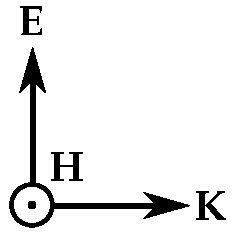
\includegraphics[width=.12\textwidth]{img/tripletEHK.pdf}}
\end{overpic}\qquad
\end{figure}

%}}}
\paragraph{Symmetry of the split-ring}%{{{
The orientation of the splitting in the SRR determines the possible coupling between its electric and magnetic dipoles. In particular, when the splitting is on the front or rear side of the ring relative to the  direction of wave propagation, the predominantly magnetic resonance creates also a weak electric dipole, leading to the optical activity.

Reduced symmetry with regards to the wave propagation may even break the homogenisation based on scattering parameters retrieval, as this procedure assumes that the structure is symmetric, i.e., its reflectance is equal from both sides. Asymmetric structures therefore have properties that can not be matched by any (reciprocal) homogeneous medium. 

The symmetry is restored again by considering a \textit{symmetric split ring resonator} (sSRR), depicted in Fig. \ref{fg_SRR_types}b, which has two splittings at opposing position on the ring. 
% A. Andryieuski, C. Menzel, C. Rockstuhl, R. Malureanu, and A.V. Lavrinenko, The split cube in a cage: %bulk negative-index material for infrared applications, Journal of Optics A: Pure and Applied Optics,
%vol. 11, p. 114010, 2009.
This is documented by the results in \ref{fg_SRR_principles}. The SRR with a single splitting is represented by red lines; while its magnitude of reflectance and transmittance in Fig. \ref{fg_SRR_principles}a,b appear similar to these of a cut wire, the computation of the refractive index yields a spectrum (Fig. \ref{fg_SRR_principles}c) which has no reasonable interpretation near the resonance at 500 GHz and above it. 

The symmetric resonator is represented by green curves. In Fig. \ref{fg_SRR_principles}c, the refractive index follows a resonance pattern that was already described on the example of the cut wires: the curve grows up to the upper Brillouin zone boundary, follows it for a span of frequencies, drops to the Brillouin zone boundary below, follows it again and then a next band starts. 

At higher frequencies, outside the range of Fig. \ref{fg_SRR_principles}, the SRR exhibits also the electric resonance where the current flows symmetrically along both its arms. It is assumed that any structure should support infinite number of resonances, of which only the lowest few are usually of any interest.
%}}}
\paragraph{Antiresonances in local effective parameters}%{{{
In the case of symmetric split-ring resonators, the first resonance possesses only the magnetic dipole moment, as follows from the symmetry of the resonant fields. This fact reflects in a strong resonant behaviour of the permeability $\meff(f)$ (green curve in Fig. \ref{fg_SRR_principles}e, between 600 and 700 GHz). 

The permittivity spectrum $\eeff(f)$ is, however, also affected by the magnetic dipole resonance  (Fig. \ref{fg_SRR_principles}d). The impact of the magnetic resonance on $\eeff(f)$ is several times weaker than on $\meff(f)$, and more importantly, it has an opposite sign: The real part of $\eeff'(f)$ is reduced at frequencies below the resonance, and increased above it. Simultaneously, the sign of the imaginary part $\eeff''(f)$ would imply amplification of the electric field oscillating around 650 GHz, which is impossible in a structure composed of lossy materials only. This feature in the spectrum is sometimes described as an \textit{antiresonance} and has incited much discussion in the literature \cite{koschny2003resonant, wallen2011anti}. 
%}}}
\paragraph{Physical relevance of effective parameters in their local approximation}%{{{
We believe that the influence of a magnetic resonance on $\eeff(f)$, or conversely, of an electric resonance of $\meff(f)$, is a mere artifact of approximating a strongly nonlocal structure with a concept of local effective parameters. It can be shown antiresonances become stronger at higher frequencies, as the wavelength $2\pi/K$ becomes similar to the unit cell size $a$. 
In Ref. \cite{wallen2011anti}, it is argued that % against this interpretation with
\begin{displayquote}
\textit{the periodicity cannot \ldots be the only explanation since qualitatively similar antiresonances have been reported using the measured data for a disordered high permittivity composite.}
\end{displayquote}
The true origin of antiresonances and other deviations of $\eeff(f)$ and $\meff(f)$ from the Lorentzian resonance curve can however be attributed to the presence of photonic band gaps and nonlocal response of the structure. These effects are, to some extent, maintained also under randomizing the unit cell positions \cite{peng2007},   
and there is probably no need to seek for another explanation. %%TODO rewiew, rewrite?
% \cite{alu2010} "Restoring the physical meaning of MM constitutive parameters"

%An elaborate comparison of resonant metallic structures, with clear effect of adding the wire to the transmission spectra, can be found e.g. in Ref. \cite{koschny2004effective}.

%Ref. \cite{li2009determination} contains typical complex-valued spectra of $\eeff$ and $\meff$ for a SRR and SRR-Wire
% different orientations - some leading to chirality i.e. linear dependence of f(K)
% when not failing due to chirality, s-param yields beautifully similar results to our simulations!
% "CMM = Composite MetaMaterial"
%}}}
\paragraph{Comparison of the s-parameters method and current-driven homogenisation}%{{{
With local effective parameters $\eeff(f)$ and $\meff(f)$ appearing to lose their physical meaning in a frequency range near a resonance, a question remains to what extent the dispersion curves, or equivalently, the spectrum of effective index of refraction $\Neff(f)$ is applicable. While the Bloch theorem in Eq. (\ref{eq_bloch}) suggests that the dispersion curves for the Bloch wavevector $\KK$ can be determined for any periodic structure, the s-parameter method might return invalid values.

Dispersion curves obtained by the s-parameters method and by the current-driven homogenisation (CDH) are compared in Fig. \ref{fg_cdh5}. Although these methods are fundamentally different, their results overlap, and thus one can assume that the array of symmetric split-ring resonators can be treated as homogeneous with well-defined index of refraction $\Neff(f)$ for the Bloch wave over the whole spectrum. Its local effective parameters $\eeff(f)$ and $\meff(f)$, however, seem to have no useful physical interpretation near the resonances, where the Bloch wavelength is similar to the unit cell size. They remain useful farther from the resonance, though. % todo perhaps add some particular frequency ranges from the Fig.

%}}}
\paragraph{Variants of split-ring resonators}%{{{
\begin{figure}[t] \caption{Other variants of split-ring resonators: \textbf{(a)} double SRR, \textbf{(b)} symmetric version thereof, \textbf{(c)} double SRR with cross-connection between the inner and outer rings, \textbf{(d)} illustration of a square variant of the double SRR, \textbf{(e)} the "omega" structure aimed to introduce $\Neff'<0$, \textbf{(f)} the cut-wire pair} \label{fg_SRRothers} \centering 
\begin{overpic}[height=0.22\textwidth]{img/drawing_dSRRpad.pdf}    \put (1,81) {\textbf{(a)}}\end{overpic}\quad
\begin{overpic}[height=0.22\textwidth]{img/drawing_dsSRRpad.pdf}   \put (1,81) {\textbf{(b)}}\end{overpic}\quad
\begin{overpic}[height=0.22\textwidth]{img/drawing_dSRRcrossed.pdf}\put (1,81) {\textbf{(c)}}\end{overpic}\\
\begin{overpic}[height=0.22\textwidth]{img/drawing_dSRRsquare.pdf} \put (-7,81) {\textbf{(d)}}\end{overpic}\quad
\begin{overpic}[height=0.22\textwidth]{img/drawing_SRRomega.pdf} \put (-6,81) {\textbf{(e)}}\end{overpic}\quad
\begin{overpic}[height=0.22\textwidth]{img/drawing_strippair.pdf} \put (1,81) {\textbf{(f)}}
		\put(100,30){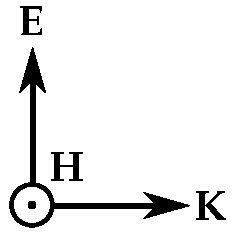
\includegraphics[width=.12\textwidth]{img/tripletEHK.pdf}}
\end{overpic}\quad
\end{figure}
Diverse metamaterial designs based on the SRR principle were developed.
Many SRR designs involve a smaller ring nested inside the original one, as shown in Fig. \ref{fg_SRRothers}a,b in the asymmetric and symmetric variants. The long narrow gap between the inner and outer split ring enhances their capacitive coupling. This way, the frequency of the magnetic resonance can be reduced without increase of the overall SRR dimensions. Such designs usually do not need capacitor pads, and can be made by etching or microlitography. 

A modification of this \textit{double split-ring} design includes cross-connection between the inner and outer conductors as in Fig. \ref{fg_SRRothers}c; this version also breaks mirror symmetry. 

The square "ring" resonator (Fig. \ref{fg_SRRothers}d) is also widely used, without any substantial difference from the round SRR.

The \textit{omega structure} was designed to emulate the operation of a SRR and a wire simultaneously \cite[pp. 62--72]{croenne2009controle}, by interconnecting the ends of a SRR along the $x$-axis (Fig. \ref{fg_SRRothers}e).

All SRR structures in Fig. \ref{fg_SRRothers} can be made flat in the plane perpendicular to the magnetic field, which facilitates their fabrication. At terahertz and higher frequencies, using a thin metal film should not be much detrimental to the SRR conductivity, since the skin depth caused by eddy currents is often submicroscopic \cite{gibbons2010scalable}.

On the contrary, a similar way of operation is achieved by structures infinite in the direction of the magnetic field. This allows to fabricate magnetic resonators by rolling stripes of a semi-metallised plastic foil, producing a \textit{swiss-roll} metamaterial \cite{gibbons2010scalable}, or by partially sputter-coating a polymer fibre by metal \cite{wang2011fiber}. Such structures however seem to exhibit relatively high losses when applied above the microwave range.

Metallic \textit{cut-wire pair}, or also \textit{strip pair}, metamaterial depicted in Fig. \ref{fg_SRRothers}f, was designed for operation in the infrared or optical range. It can be understood as a split-ring resonator flattened along the direction of the wave vector. The geometry is tuned so that the electric and magnetic resonances overlap.	

%}}}
\paragraph{SRR in a wire array} %{{{
The analysis of the wire array has shown that at low frequencies, its effective permittivity is physically valid and has a negative value. Likewise, the symmetric SRR has a region in the spectrum above its magnetic resonance where its effective permeability is negative, too.

A synthesis of these two structures yields a region of negative index of refraction, probably the first \cite{pendry2000negative} and most prominent metamaterial design to achieve this. The effect of combining structures that interact exclusively with magnetic and electric field is discussed in Ref. \cite{koschny2004effective} in more detail.

The resulting effective parameters are represented by the blue line in Fig. \ref{fg_SRR_principles}. Its spectrum of the effective index of refraction resembles that of the wire array up to 630 GHz, where it drops by one Brillouin zone down at the resonant frequency.
By rule, a single individual resonance always causes $\Neff'(f)$ to drop from one Brillouin zone boundary to another, which should be observed in all correctly retrieved spectra. 

Notice that the magnetic resonance causes a drop in $\Neff'(f)$ even without the wire array (green curve in Fig. \ref{fg_SRR_principles}c), but in such a case it happens between the first Brillouin zone boundary and zero. Without wires, $\Neff'$ does not reach negative values.

By contrast, a magnetic resonance in the combined SRR-wire structure introduces a narrow region, still within the photonic band gap, where 
\begin{equation} \Neff(f) = -\frac{c}{2 a f}, \label{eq_BZN2}\end{equation}
with $a$ being the unit cell size.	
This means that the photonic band spanning from 635 to 670 GHz has $\Neff'<0$, but the effective permittivity and permeability can be attributed with physical meaning only when $\Neff'$ comes closer to zero, roughly from 650 to 670 GHz. They are correctly retrieved as both negative, as can be indeed seen from in Figs. \ref{fg_SRR_principles}d,e (blue lines).

%}}}
\paragraph{Fano resonance} %{{{
The spectrum of reflectance magnitude $|r(f)|$ for the sSRR-wire structure (blue line in Fig. \ref{fg_SRR_principles}a) has a relatively complex shape -- starting from a high reflectance introduced by the wire array, it grows below the magnetic resonance, then it drops to zero around 660 GHz, and it grows until its local maximum on 750 GHz is reached.

The line shape differs significantly from the arguably simpler spectrum of the cut wires (Figs. \ref{fg_CutWires_wireradius1u_cutwidth_comparison}a and \ref{fg_CutWires_wirecut2um_wireradiusscan}a), where the resonance was accompanied by a single peak in reflectance. 
The reason is in that with the sSRR-wire structure, $|r(f)|$ is a linear superposition of the wave scattered by the interaction of the structure with the electric field, which has relatively large amplitude $r_{1}(f)$ over broad spectral range, and another wave $r_{2}(f)$ scattered by the magnetic dipole which is prominent only close to the magnetic resonance, between 550 and 750 GHz.

Both scattered components, $r_1(f)$ and $r_2(f)$, are complex functions. The phase of a wave scattered by a resonant element differs almost by $\pi$ for $f$ below and above the resonance. The impact on the plot of the overall reflectance is in a change from a constructive to destructive interference between the two components. 

Such typical spectral features, observed whenever a narrower resonance overlaps with another broader one, are known as \textit{Fano resonances}, and can be found on most following plots of $|r(f)|$ or $|t(f)|$. The Fano lineshape is a natural interference between waves scattered by different mechanisms: whenever the spectrum of a structure close to a magnetic dipole resonance does not fall into the class of possible Fano lineshapes, it suggests the homogenization has failed. For an example, see the spectra of the asymmetric SRR in \ref{fg_SRR_principles}.  
%Complementary observations can be made with the transmission spectrum, as both kinds of structures have negligible losses.

%}}}
\begin{figure}[t] \caption{Split-ring resonator: %{{{
		amplitude of \textbf{(a)} reflectance, \textbf{(b)} transmittance, \textbf{(c)} effective index of refraction,  \textbf{(d)} effective permittivity $\eeff$ and \textbf{(e)} effective permeability $\meff$  .   %% todo check params comment=sSRR with wire_resolution=2.000e-06_capacitorr=1.000e-05_splitting=4.000e-06_wirethick=4.000e-06_splitting2=4.000e-06_radius=3.000e-05_simtime=2.000e-10
Outer ring radius $\rho = 30$ $\mu$m, conductor cross-section $\Delta\rho = 6$ $\mu$m, unit cell size $a=100$ $\mu$m. \\
Comparison of the more familiar standard SRR (split width $d=4$ $\mu$m) with its symmetric variant sSRR (double split width $d=2$ $\mu$m) and the same sSRR with wire grid added. The dispersion curves nor effective parameters for the asymmetric SRR could not be determined by the scattering parameters method. } \label{fg_SRR_principles} \centering \vspace{-3mm} 
\begin{tabular}{r}
\begin{overpic}[width=0.85\textwidth]{img-meep/SRR_principles_r.pdf} \put (-1,28) {\textbf{(a)}} \end{overpic}\vspace{-0.060\textwidth}\\
\begin{overpic}[width=0.85\textwidth]{img-meep/SRR_principles_t.pdf} \put (-1,28) {\textbf{(b)}} \end{overpic}\vspace{-0.060\textwidth}\\
\begin{overpic}[width=0.85\textwidth]{img-meep/SRR_principles_n.pdf}\put (-1,28) {\textbf{(c)}} \end{overpic}\vspace{-0.060\textwidth}\\
\begin{overpic}[width=0.85\textwidth]{img-meep/SRR_principles_eps.pdf}\put (-1,28) {\textbf{(d)}} \end{overpic}\vspace{-0.060\textwidth}\\
\begin{overpic}[width=0.85\textwidth]{img-meep/SRR_principles_mu.pdf}\put (-1,28) {\textbf{(e)}} \end{overpic}\vspace{-0.030\textwidth}\\
\end{tabular}
\end{figure}
\begin{figure}[h] \caption{Current-driven homogenization results, shown as bubbles,  indicating the dispersion curves 
	for \textbf{(a)} a symmetric split-ring resonator and \textbf{(b)} the same with a wire mesh. The results of the scattering-parameters method are overlayed as green lines; these show the same data as the green and blue solid lines from Fig. \ref{fg_SRR_principles}c. In the right panel, the negative-index range of frequencies between 630 and 670 GHz was mirrored against the $K=0$ vertical axis and plotted by a dashed green line.} \label{fg_cdh5} \centering  % todo add params SRRArray_comment=symmetric SRR_simtime=2.000e-10_wirethick=0.000e+00_splitting2=1.600e-05_radius=3.000e-05_model=SRRArray.pdf
	% TODO recalculate and update
	\vspace{.1\textwidth}
	\begin{overpic}[width=.48\textwidth]{img-cdh/cdh_sSRR.pdf}  
	\put(1,96) {\textbf{(a)}} 
	\put(18,100){
\includegraphics[width=.1\textwidth]{img/drawing_sSRRpad.pdf}}
	\put(31,105){sSRR}
	\end{overpic}
	\begin{overpic}[width=.48\textwidth]{img-cdh/cdh_sSRR_wire.pdf}  
	\put(16,100){
\includegraphics[width=.1\textwidth]{img/drawing_sSRRpad_wire.pdf}}
	\put(29,105){sSRR + wire}
	\put(1,96) {\textbf{(b)}} 
	\end{overpic}
\end{figure}

% todo possibly recalculate CDH for the SRR as in \ref{fg_SRR_principles}
%\begin{figure}[h] \caption{Current-driven homogenization results for the split-ring resonator \textbf{(a)} without the wire mesh and \textbf{(b)} with the wire mesh. 
	%} \label{fg_cdh4} \centering 
	%\begin{overpic}[width=.48\textwidth]{img-cdh/cdh_SRR.pdf}  \put(1,96) {\textbf{(a)}} \end{overpic}
	%\begin{overpic}[width=.48\textwidth]{img-cdh/cdh_SRRWire.pdf}  \put(1,96) {\textbf{(b)}} \end{overpic}
%\end{figure}
%}}}
\FloatBarrier %====================================================================================================
%}}}
\section{Combined electric and magnetic resonator} \label{section_srr} %{{{
\paragraph{Effect of the central bar in SRR}%{{{
The fundamental resonance of a split-ring resonator (SRR) is the magnetic one, where the current circulates around its circumference. When one adds a central bar parallel to the electric field and the $x$-axis, as in Fig. \ref{fg_SRR_elmag}a, the frequency of the magnetic resonance does not change significantly. The reason comes from the symmetry thereof, which stipulates that that zero net current flows through the central bar. 

However, a new electric resonance (Fig. \ref{fg_emcSRR_resonances}b) is introduced by adding the bar, characteristic by that the current conducted by the central bar is antiparallel to the current conducted by both SRR arms. The corresponding frequency is lower compared to the original parallel electric resonance (Fig. \ref{fg_emcSRR_resonances}c), and similar to the frequency of the magnetic resonance (Fig. \ref{fg_emcSRR_resonances}a).  
\begin{figure}[h] \caption{\textbf{(a)} A modification of a split-ring resonator with a central bar, \textbf{(b)} a similar structure where the central bar was split by a capacitor with pad radius $\rho_c$, allowing to tune the antiparallel electric resonance} \label{fg_SRR_elmag} \centering 
\begin{overpic}[height=0.25\textwidth]{img/drawing_eSRRpad.pdf}\put (1,80) {\textbf{(a)}}\end{overpic}\quad\quad\quad
\begin{overpic}[height=0.25\textwidth]{img/drawing_emcSRRpad_sizes.pdf}\put (1,80) {\textbf{(b)}}\end{overpic}
\end{figure}
\begin{figure}[b] \caption{Three low-frequency resonances in the combined SRR: \textbf{(a)} magnetic resonance, \textbf{(b)} antiparallel electric resonance, \textbf{(c)} parallel electric resonance.\\ The actual order of the first two resonances in the spectrum is determined by the inner capacitor radius $\rho_c$ or other parameters of the structure.} \label{fg_emcSRR_resonances} \centering 
\begin{overpic}[height=0.22\textwidth]{img/drawing_emcSRRpad_resM.pdf}\put (1,81) {\textbf{(a)}}\end{overpic}\quad
\begin{overpic}[height=0.22\textwidth]{img/drawing_emcSRRpad_resE2.pdf}\put (1,81) {\textbf{(b)}}\end{overpic}\quad
\begin{overpic}[height=0.22\textwidth]{img/drawing_emcSRRpad_resE2b.pdf}\put (5,54) {\textbf{(c)}}
		\put(100,10){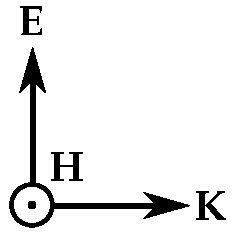
\includegraphics[width=.1\textwidth]{img/tripletEHK.pdf}}
\end{overpic}\qquad\quad
\end{figure}

%}}}
\paragraph{Tuning the frequency of the antiparallel electric resonance}%{{{
The spectra of the cut wires (Fig. \ref{fg_CutWires_wireradius1u_cutwidth_comparison}) suggest that each electric resonance, if not preceded by a Bragg band gap or excessively lossy, introduces a region in spectrum where the local effective permittivity has a physically meaningful and negative value. Under the same condition in Fig. \ref{fg_SRR_principles}, the magnetic resonance introduces a region of $\meff(f) < 0$.
\begin{figure}[t] \caption{Combined electric-magnetic resonator: amplitude of \textbf{(a)} reflectance, \textbf{(b)} transmittance and \textbf{(c)} effective index of refraction $\Neff = \Neff' + \ii \Neff''$.  
% todo check the structure parameters
%Outer ring radius $\rho = 30$ $\mu$m, conductor cross-section $\Delta\rho = 6$ $\mu$m, unit cell size $a=100$ $\mu$m. \\
%Comparison of the more familiar standard SRR (split width $d=4$ $\mu$m) with a symmetric SRR (double split width $d=2$ $\mu$m) and the same symmetric SRR with wire grid added.  The effective parameters for the asymmetric SRR could not be determined by the scattering parameters method.  %TODO params and comment 
The frequency of the electric resonance is influenced by the radius $\rho_c$ of the capacitor on the central spoke.
} \label{fg_emSRR_icr} \centering \vspace{-3mm} 
\begin{tabular}{r}
\begin{overpic}[width=0.85\textwidth]{img-meep/emSRR_inner_capacitor_radius_scan_r.pdf} \put (-1,28) {\textbf{(a)}} \end{overpic}\vspace{-0.060\textwidth}\\
\begin{overpic}[width=0.85\textwidth]{img-meep/emSRR_inner_capacitor_radius_scan_t.pdf} \put (-1,28) {\textbf{(b)}} \end{overpic}\vspace{-0.060\textwidth}\\
\begin{overpic}[width=0.85\textwidth]{img-meep/emSRR_inner_capacitor_radius_scan_n.pdf} \put (-1,28) {\textbf{(c)}} \end{overpic}\vspace{-0.030\textwidth}\\
\end{tabular}
\end{figure}

By optimizing the structure geometry, the resonances can be tuned against each other so that the regions of $\eeff(f) < 0$ and $\meff(f) < 0$ overlap. This is the conventional approach to design a metamaterial with a negative index of refraction; applying it to the electro-magnetic resonator leads to an array of independent, nonconnected elements, which may be an advantage over embedding SRRs in a wire array. One of the means of tuning the antiparallel electric resonance frequency is to divide the central bar by an \textit{inner} capacitor as shown in Fig. \ref{fg_SRR_elmag}b. 

For the inner capacitor being relatively small, with radius $\rho_c = 6$ $\upmu$m, the electric resonance is located around 1150 GHz, and it shifts down to 940 GHz when $\rho_c$ is increased to 8 $\upmu$m. On the contrary, the magnetic resonance is virtually independent of $\rho_c$ and remains close to 800 GHz. Both individual resonances can be clearly identified as points of zero transmission and as corresponding steep, but still continuous, drops in the refractive index (red and light green curves in Fig. \ref{fg_emSRR_icr}).  For $\rho_c \leq 8$ $\upmu$m, the resonances are separated by a photonic band, indicating that the regions of  $\eeff(f) < 0$ and $\meff(f) < 0$ do not overlap. 

An attempt to further reduce the frequency of the electric resonance to obtain negative index of refraction $\Neff'<0$ in the region of overlap, however, leads to confusing results (cyan curves in Fig. \ref{fg_emSRR_icr}). 
For $\rho_c \in \langle10, 16\rangle$ $\upmu$m, the scattering parameters method retrieves apparently erroneous spectra with two disticnct band gaps, but without any individual resonance.
A more detailed parametric scan through these problematic values of $\rho_c$ can be found in Fig. \ref{fg_emSRR_icrscan}.

\begin{figure}[t] \caption{\textbf{(a)} Reflectance and \textbf{(b)} the imaginary part of the refractive index, as questionably retrieved by the scattering parameters method, for the electro-magnetic split-ring resonator} \label{fg_emSRR_icrscan} \centering 
\begin{overpic}[width=0.48\textwidth]{img-meep/emSRR_inner_capacitor_radius_scan_HR_r.pdf}\put(-1,80){\textbf{(a)}}\end{overpic}
\begin{overpic}[width=0.48\textwidth]{img-meep/emSRR_inner_capacitor_radius_scan_HR_ni.pdf}\put(-1,80){\textbf{(b)}}\end{overpic}  
\end{figure}

The effective parameters retrieved by the s-parameters method become easy to interpret for $\rho_c \geq 18$ $\upmu$m. The antiparallel resonance at 690 GHz is again well separated from the magnetic one, which remains near its original frequency (dark blue curves in Fig. \ref{fg_emSRR_icr}). Further explanation of these results is beyond the capabilities of the scattering parameters method, and necessitate the more expensive computation using the current-driven homogenisation (CDH).

%}}}
\begin{figure}[t] \caption{Current-driven homogenization results for the combined electric-magnetic resonator, differing by the inner capacitor radius \textbf{(a)} $\rho_c = 6$ $\mu$m, \textbf{(b)} $\rho_c = 8$ $\mu$m.} \label{fg_cdh1} \centering %{{{
	\vspace{.1\textwidth}
	\begin{overpic}[width=.48\textwidth]{img-cdh/cdh_emcSRRcap06.pdf}  
	\put(1,96) {\textbf{(a)}} 
	\put(18,100){
\includegraphics[width=.1\textwidth]{img/drawing_emcSRRpad.pdf}}
	\put(30,105){$\rho_c = 6$ $\upmu$m}
	\end{overpic}
	\begin{overpic}[width=.48\textwidth]{img-cdh/cdh_emcSRRcap08.pdf}  
	\put(18,100){
\includegraphics[width=.1\textwidth]{img/drawing_emcSRRpad.pdf}}
	\put(30,105){$\rho_c = 8$ $\upmu$m}
	\put(1,96) {\textbf{(b)}} 
\end{overpic}
\end{figure}
%}}}
\paragraph{Current-driven homogenization and spatial dispersion}%{{{
CDH results for the same structure parameters, $\rho_c\in\{6,8,10,18\}$ $\upmu$m are presented in Figs. \ref{fg_cdh1} and \ref{fg_cdh2}. For comparison, the dispersion curves corresponding to the $\Neff'(f)$ retrieved by the scattering parameters method are shown as green curves.

For $\rho_c=6$ $\upmu$m, both retrieval methods give relatively similar results, and they correctly identify two indirect band gaps corresponding to the magnetic and antiparallel electric resonances, respectively. The match is not as good as in Fig. \ref{fg_cdh5}, though -- namely the magnetic resonance around 800 GHz appears somewhat wider when retrieved by the s-parameters method, compared to CDH. The deviation can be attributed to the structure being surrounded by vacuum instead of sensing the near fields of the surrounding cells (c.f. page \pageref{cdhadvantages}).

The next plot for $\rho_c=8$ $\upmu$m was not chosen randomly, since for this inner capacitor radius, the spatial dispersion starts to substantially affect the dispersion curve of the second photonic band. It starts in the $\mathbf \Gamma$ point at 794 GHz with a positive group velocity, reaches its maximum of 890 GHz, then the group velocity changes its sign and the band ends in the $\mathbf X$ point at ca. 887 GHz. At a given frequency between 887 and 890 GHz, two solutions of the wave equation exist that differ merely by the wavevector. The s-parameters method has no means of distinguishing them, and accordingly the retrieved dispersion curve deviates from that retrieved by CDH.

Spatial dispersion is even more evident in Fig. \ref{fg_cdh2} where the frequencies of the $\mathbf \Gamma$ and $\mathbf X$ points come close to each other, i.e. 784 and 795 GHz, respectively. The central maximum of the band is on 828 GHz, which explains why the s-parameters	method no longer determines the dispersion curve shape correctly, nor it identifies any of the resonances.

These issues persist until $\rho_c \geq 18$ $\upmu$m, when the second photonic band becomes a relatively flat function of the wavenumber $K$. Both resonances are then again retrieved correctly, except for a systematic error in the frequency determination which may arise from the already discussed difference in the simulation geometry used by the s-parameters method.

%}}}
\begin{figure}[t] \caption{Current-driven homogenization results for the combined electric-magnetic resonator, differing by the inner capacitor radius \textbf{(a)} $\rho_c = 10$ $\mu$m, \textbf{(b)} $\rho_c = 18$ $\mu$m.} \label{fg_cdh2} \centering %{{{
	\vspace{.1\textwidth}
	\begin{overpic}[width=.48\textwidth]{img-cdh/cdh_emcSRRcap10.pdf}  
	\put(1,96) {\textbf{(a)}} 
	\put(18,100){
\includegraphics[width=.1\textwidth]{img/drawing_emcSRRpad.pdf}}
	\put(30,105){$\rho_c = 10$ $\upmu$m}
	\end{overpic}
	\begin{overpic}[width=.48\textwidth]{img-cdh/cdh_emcSRRcap18.pdf}  
	\put(18,100){
\includegraphics[width=.1\textwidth]{img/drawing_emcSRRpad.pdf}}
	\put(30,105){$\rho_c = 18$ $\upmu$m}
	\put(1,96) {\textbf{(b)}} 
	\end{overpic}
\end{figure}
%}}}
\paragraph{Is this a negative-refraction structure?}%{{{
The electro-magnetic resonator was examined as an example structure which, particularly in its magnetic resonance, exhibits strong electric quadrupole, leading to prominent spatial dispersion. Figures \ref{fg_cdh1} and \ref{fg_cdh2} illustrated that not only the s-parameters retrieval algorithm fails, but also the very idea of describing the structure behaviour in terms of refractive index $\Neff(f)$ does not guarantee enough degrees of freedom to express the physical reality.
Similar failure of the s-parameters method in homogenization of an array of SRRs in a wire lattice was reported previously, \cite{rockstuhl2008transition}, showing that $\Neff(f)$ can be determined only for relatively big spacing between the metallic  elements.
% ... and maybe this was noted by Silveirinha2009
% Nonlocal homogenization of an array of cubic particles made of resonant rings

For particular values of the inner capacitor radius $\rho_c \in \langle8,16\rangle$ $\upmu$m, the second photonic band supports simultaneously a wave of group velocity collinear with the phase velocity, and an \textit{additional wave} with higher wavenumber and opposite direction of these velocities. 

Provided the auxiliary boundary conditions are arranged to couple all energy exclusively to this additional wave, with the relatively high Bloch wavevector, the interface of the metamaterial with vacuum should indeed exhibit negative refraction. The index of refraction, however, is not sufficient for description of this kind of metamaterial -- even for propagation parallel to the optical axis.

%}}}
\FloatBarrier %====================================================================================================
%}}}
\section{Dielectric spheres} %{{{
% \cite{prosvirnin2015planar} % todo read
\paragraph{Mie resonances}%{{{
Already in Eqs. (\ref{eq_rho_n1},\ref{eq_rho_n2}) it was assumed that at higher frequencies, there is no difference in the effect of conduction and polarisation currents. The current conducted around a split-ring resonator has a direct analogy in the polarisation current circulating along the circumference of a dielectric particle. The capacitor of the SRR is then replaced by the distributed capacitance of the whole dielectric. For the first resonance in spherical dielectric particles, the magnetic dipole moment induced by the polarisation current goes through the sphere axis. The resonance frequency is inversely proportional to the radius $\rho$ of the sphere, and in general, decreases monotonously with the growth of the dielectric permittivity $\epsrl$.

The second resonance has an electric dipole moment. It is similar to the magnetic one, but the electric and magnetic fields exchange their topology: The magnetic field circulates around the axis of the sphere, and the polarisation current forms the electric dipole. Although the topology of both resonances is the same, the resonance frequency of the magnetic one is lower, since the electric field is then almost entirely confined to the dielectric volume, whereas for the electric resonance, most of the streamlines of the electric field have to pass through the surrounding air.
%merlin2009metamaterials

\begin{figure}[h]  %% fg_Spheres_lossscan
	\caption{The electric field component $E_x$ (shaded in blue-white-red) and magnetic field components $H_y,H_z$ (plotted as vectors) for \textbf{(a)} the magnetic and \textbf{(b)} electric Mie resonance in a dielectric sphere. The figure is in the $y$-$z$ plane of mirror symmetry, so the fields have no other nonzero components than shown here. On the right side, the vectors depict right-hand field triplet of the incident plane wave.}  \centering 
	\begin{overpic}[width=.35\textwidth]{img/sphere_Mie_mode_magnetic.pdf}  \put(1,93) {\textbf{(a)}} \end{overpic}
    \begin{overpic}[width=.35\textwidth]{img/sphere_Mie_mode_electric.pdf}  \put(1,93) {\textbf{(b)}} 
		\put(100,30){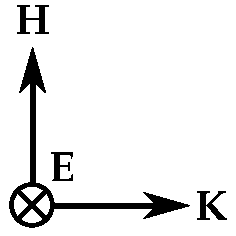
\includegraphics[width=.12\textwidth]{img/tripletHEK.pdf}}
	\end{overpic}
\label{fg_Mie}  \end{figure}

An analytic theory of electromagnetic resonances in dielectric spheres (or rods) was developed by Mie in 1908 \cite{mie1908beitrage}, and correspondingly they are denoted as \textit{Mie resonances}. 
Dielectric resonators operate in a similar way to a series L-C circuit, as was noticed by Richtmyer in 1939 \cite{richtmyer1939dielectric}. Few decades later, the dielectric resonator found its use in the developing microwave technology; usually it takes the form of a millimeter-sized ceramics disc glued to the microstrip circuits. 
The Mie theory describes the scattering from a single particle surrounded by vacuum, but for high enough dielectric permittivity $\epsrl \gtrsim 50$, the resonant fields are well confined in the dielectric volume and are not much affected by the presence of the neighbouring cells.
An artificial dielectric consisting of dielectric particles with effective permeability differing from unity was considered by Lewin in 1947 \cite{lewin1947electrical}; apparently it was not until 2002 when O'Brien et al. computed \cite{obrien2002photonic} that the effective permeability of such a structure may be negative.
\label{negn_diel}


Infinite number of the higher-order resonances exist \cite[pp. 407-408]{mie1908beitrage}, resembling the set of single-electron orbitals around an atomic nucleus. Many of these, e.g. most \textit{d}-type orbitals, have zero electric or magnetic dipole moments. Dipole moments of many others exist, but are not oriented parallel to the fields of the incident wave, and do not couple to the electromagnetic wave. In the spectrum of an array of dielectric spheres, one can clearly identify the remaining resonances as the most prominent magnetic one, electric one, the second magnetic, second electric etc. The first three resonances from this alternating series are shown in Fig. \ref{fg_Spheres_lossscan}, each manifesting as a peak in reflectance, and as a pair of resonance in $\meff(f)$ and antiresonance in $\meff(f)$, or vice versa.

%% todo cite vendik, Zhao etc. from the directory

%}}}
\begin{figure}[h!] %fg_Spheres_lossscan %{{{
	\caption{Amplitude of \textbf{(a)} reflectance, \textbf{(b)} transmittance and \textbf{(c)} effective index of refraction $\Neff = \Neff' + \ii \Neff''$ of TiO$_{2}$ spheres with varied loss compared to the natural one from Ref. \cite{baumard1977_epsilon_TiO2}; sphere radius $\rho = 30$ $\mu$m, unit cell size $a=100$ $\upmu$m.} \label{fg_Spheres_lossscan} \centering \vspace{-0.0\textwidth} 
\begin{tabular}{r}
\begin{overpic}[width=0.85\textwidth]{img-meep/Spheres_lossscan_r.pdf}  \put (-1,28) {\textbf{(a)}} \end{overpic}\vspace{-0.060\textwidth}\\
\begin{overpic}[width=0.85\textwidth]{img-meep/Spheres_lossscan_t.pdf}  \put (-1,28) {\textbf{(b)}} \end{overpic}\vspace{-0.060\textwidth}\\
\begin{overpic}[width=0.85\textwidth]{img-meep/Spheres_lossscan_n.pdf}  \put (-1,28) {\textbf{(c)}} \end{overpic}\vspace{-0.060\textwidth}\\ 
\begin{overpic}[width=0.87\textwidth]{img-meep/Spheres_lossscan_eps.pdf}\put (-1,28) {\textbf{(d)}} \end{overpic}\vspace{-0.060\textwidth}\\
\begin{overpic}[width=0.87\textwidth]{img-meep/Spheres_lossscan_mu.pdf} \put (-1,28) {\textbf{(e)}} \end{overpic}\vspace{-8mm}\\
\end{tabular}
\end{figure}
%}}}
\paragraph{Dielectric losses}%{{{
Unlike split-ring resonators, where the high-frequency dissipative losses depend on many factors such as the eddy currents and details in the geometry, the losses in dielectric resonators are well defined and their effect can be reliably computed by the FDTD simulation. 

We used a realistic model \cite{baumard1977_epsilon_TiO2} of polycrystalline rutile (TiO$_{2}$). The relative permittivity of rutile was already plotted in Fig. \ref{fg_tio2eps}; in the terahertz range it classifies as a high-permittivity dielectric with a relatively low losses, compared to other similar materials:

\begin{equation}\epsrl(f=1\text{ THz}) = 94.2-2.43\text{i}. \label{eq_tio2}\end{equation}
The actual permittivity of the experimentally measured samples depended on their preparation, in particular the volume fraction of microscopic voids. For such composites, Ref. \cite{baumard1977_epsilon_TiO2} gives only the ratio of $\epsrl''/\epsrl'$, but since $\epsrl'$ could be determined from the resonance frequencies in the experimental spectra, also the imaginary part could be easily computed.

The reflectance, transmittance and effective parameters of rutile spheres with radius $\rho=15\;\upmu$m are shown in Fig. \ref{fg_Spheres_lossscan}. Three different levels of losses were considered, with the realistic value represented as 100 \%, and accompanied with a hypothetic low-loss dielectric with the same real part $\epsrl'$, but the imaginary part $\epsrl''$ artificially reduced to  10 \% and 1 \%. 

The magnetic resonance is located at 530 GHz and the electric one at 790 GHz, the second magnetic resonance follows at 1040 GHz. As a natural result of the Lorentzian model, the dielectric losses grow proportional to the frequency. Notice that around the resonance frequencies, the transmission grows with losses.

Taking realistic losses into account, the curves of the effective parameters in Figs. \ref{fg_Spheres_lossscan}c,d,e become smoother and approach the familiar curve of the damped oscillator in Fig. \ref{fg_oscillator_spectrum}. Strong enough losses prevent the formation of regions with negative effective parameters. Note, however, that formally $\Neff'$ can become negative \cite[pp. 12--15]{pazoutova2011dp} even when either $\eeff'>0$ or $\meff'>0$. Such a negative-index medium is however inevitably extremely lossy, which is represented by its \textit{figure of merit}
\begin{equation} \text{FOM} := \frac{\Neff'(f)}{\Neff''(f)} \lesssim 10. \label{eq_}\end{equation}

At the right hand side of the plot, for $f \sim a/(2c) \approx 1.5$ THz, the structure reaches a Bragg band gap. This kind of resonance is not appreciably affected by the losses, since most of the field energy in the Bragg resonance is concentrated in free space between the particles.

%}}}
\begin{figure}[h!] %% SphereWire_principles %{{{
	\caption{Amplitude of \textbf{(a)} reflectance, \textbf{(b)} transmittance and \textbf{(c)} effective index of refraction $\Neff = \Neff' + \ii \Neff''$ of TiO$_{2}$ spheres, wire grid array, a combined negative-index structure and its modification  with varied loss compared to the natural one from Ref. \cite{baumard1977_epsilon_TiO2}; sphere radius $\rho = 30 \upmu$m, unit cell size $a=100$ $\upmu$m.} \label{fg_SphereWire_principles} \centering \vspace{-3mm} %% TODO
\begin{tabular}{r}
\begin{overpic}[width=0.85\textwidth]{img-meep/SphereWire_principles_r.pdf}  \put (-1,28) {\textbf{(a)}} \end{overpic}\vspace{-0.055\textwidth}\\
\begin{overpic}[width=0.85\textwidth]{img-meep/SphereWire_principles_t.pdf}  \put (-1,28) {\textbf{(b)}} \end{overpic}\vspace{-0.055\textwidth}\\
\begin{overpic}[width=0.85\textwidth]{img-meep/SphereWire_principles_n.pdf}  \put (-1,28) {\textbf{(c)}} \end{overpic}\vspace{-0.050\textwidth}\\
\begin{overpic}[width=0.85\textwidth]{img-meep/SphereWire_principles_eps.pdf}\put (-1,28) {\textbf{(d)}} \end{overpic}\vspace{-0.050\textwidth}\\
\begin{overpic}[width=0.85\textwidth]{img-meep/SphereWire_principles_mu.pdf} \put (-1,28) {\textbf{(e)}} \end{overpic}\vspace{-0.050\textwidth}\\
\end{tabular}
\end{figure}

%}}}
\paragraph{Negative-index metamaterial based on dielectric spheres} %{{{
An important property of the periodic sphere array is its nearly \textit{isotropic} electromagnetic behaviour, i.e. independence of its behaviour on the wave polarisation. Its roots are in high symmetry of the dielectric sphere, and it is approximately maintained even when the spheres are arranged into a periodic lattice, provided that low frequencies are considered and that the spheres are too close. 
% todo Cai_Zhu2008-Diel_resonators_wires.pdf

Following the approach used to build a metamaterial with a negative refractive index from SRRs, it is possible to interlace the sphere array with the lattice of wires, which introduce negative permittivity. In order to maintain the approximate isotropy of the resulting structure, the wires may be parallel to the $x$- and $y$-axes to form a two-dimensional square mesh. This modification does not make any appreciable change in the low-frequency behaviour. % todo link to the wire mesh simulation

Fig. \ref{fg_SphereWire_principles} compares the already commented spectra for the sphere lattice (red line), and wire grid (blue line) with the spectra for the compound structure, which is sketched in Fig. \ref{fg_spherewire_sketch}a,c. At $f>0$, the wire grid does not reflect all energy, leading again to formation of the Fano resonance lineshapes. 

Notice in \ref{fg_SphereWire_principles} that the Fano resonances of structures with and without the wire mesh have a peculiar complementary shape. The wave reflected from the electric dipole of the wire mesh has an opposite sign than that reflected from the electric dipole of dielectric particles. Its sign determines whether the interference with the second component, scattered by the Mie resonances, would be constructive, or destructive. 

A band of negative index of refraction is formed above the magnetic Mie resonance, between 510 and 550 GHz. When the realistic model of losses in TiO$_2$ is used, the maximum figure of merit $\Neff'/\Neff'' \approx 6$ around the centre of the photonic band. This means that the metamaterial, in the optimum of the negative-index band, reduces the wave amplitude to $e^{1/6} \approx 0.84$ within one wavelength $\lambda$. 

After propagating over a distance of ca. $40\lambda$ in the metamaterial, the amplitude drops to $10^{-3}$ and the wave energy to $10^{-6}$ of the incident value. The applicability of such a metamaterial for building a macroscopic optical device is questionable. % todo \cite{zhao2009mie}

%Another way of achieving negative refractive index is in overlapping the electric and magnetic resonances \cite{holloway2003double} - similar to the el mag resonator above, has low spatial dispersion - but: tight requirements, double losses \cite{zhao2009mie}

%}}}
\paragraph{Effect of elliptic shape}%{{{
For a spherical dielectric particle, the frequencies of the magnetic and electric resonances, $f_{\text{M1}}$ and $f_{\text{E1}}$, respectively, scale inversely proportional to the radius $\rho$:
\begin{equation} f_{\text{M1}} \propto \rho^{-1}, \quad f_{\text{E1}} \propto \rho^{-1}. \label{eq_freq_rho}\end{equation}
A deviation from this rule may result from the inter-particle coupling in a very dense lattice, or from dispersion of the constituent dielectric.

When the particle is an ellipsoid with three independent semiaxes $\rho_x$, $\rho_y$ and $\rho_z$ aligned parallel to the $x$-, $y$- and $z$-axes, the resonance frequencies $f_{\text{M1}}$ and $f_{\text{E1}}$ become certain functions of these three ellipsoid parameters. For a nearly spherical shape, 
$$\rho_x \sim \rho_y \sim \rho_z,$$
both frequencies can be approximated as 
\begin{equation}  f_{\text{M1}} \propto \rho_x^{-0.4}  \rho_y^{-0.2} \rho_z^{-0.4}, \label{eq_freqM1_rhoxyz}\end{equation}
\begin{equation}  f_{\text{E1}} \propto \rho_x^{-0.15}  \rho_y^{-0.15} \rho_z^{-0.7}. \label{eq_freqE1_rhoxyz}\end{equation}
Obviously,  in both Eqs. (\ref{eq_freqM1_rhoxyz}) and (\ref{eq_freqE1_rhoxyz}), all three exponents must sum exactly to -1 so that they are compatible with the scaling rule for a sphere in Eq. (\ref{eq_freq_rho}). Their values are approximate only, as they were interpolated from batches of simulations which scanned through the ellipsoid parameters.

When the ellipsoid axes have a general orientation, the resonance frequencies remain almost the same; also the resonant modes are  preserved with respect to the ellipsoid orientation. An incident wave in such a case can excite multiple magnetic or electric Mie resonances of the same topology but different orientation, which differ slightly by their frequencies. The structure then may change the polarisation state of the wave, which is beyond the scope of this analysis.

%}}}
\begin{figure}[t]  % fg_spherewire_sketch%{{{
	\caption{Sketch of the sphere array embedded in a wire grid. \textbf{(a)} Front view of the simulated structure, \textbf{(b)} the experimental structure used in Ref. \cite{yakiyama2012terahertz}, measures are in micrometers. \textbf{(c)} and \textbf{(d)} top views of the corresponding structures} \label{fg_spherewire_sketch} \centering 
\begin{overpic}[width=0.30\textwidth]{img/SphereWire_num_xy.pdf} \put (1,81) {\textbf{(a)}}\end{overpic}\quad
\begin{overpic}[width=0.30\textwidth]{img/SphereWire_expe_xy.pdf}  \put (1,81) {\textbf{(b)}}
		\put(100,30){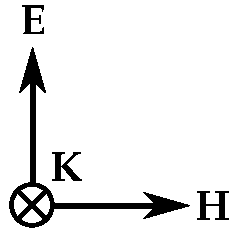
\includegraphics[width=.12\textwidth]{img/tripletEKH.pdf}}
\end{overpic}\quad \\
\begin{overpic}[width=0.30\textwidth]{img/SphereWire_num_xz.pdf} \put (1,61) {\textbf{(c)}}\end{overpic}\quad
\begin{overpic}[width=0.30\textwidth]{img/SphereWire_expe_xz.pdf}  \put (1,61) {\textbf{(d)}}
		\put(100,10){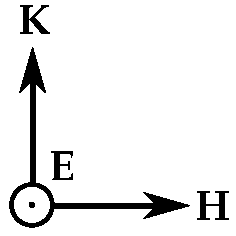
\includegraphics[width=.12\textwidth]{img/tripletKEH.pdf}}
\end{overpic}\quad
\end{figure}

%}}}
 \begin{figure}[ht]   % fg_mm2012_convolution %{{{
	 \caption{Comparison of the effective permeability $\meff(f)$ of ideal monodisperse sphere array (dashed red line), weighted average according to the size distribution (solid black line) and experimental data (green dots). \textbf{(a)} Real part of effective permeability for a sample denoted as having the "40-50" $\mu$m diameter, \textbf{(b)} for another sample with slightly larger average diameter, also depicted in Fig. \ref{fg_microphoto}. \textbf{(c)}, \textbf{(d)} corresponding imaginary parts of $\meff(f)$}
\label{fg_mm2012_convolution} \centering 
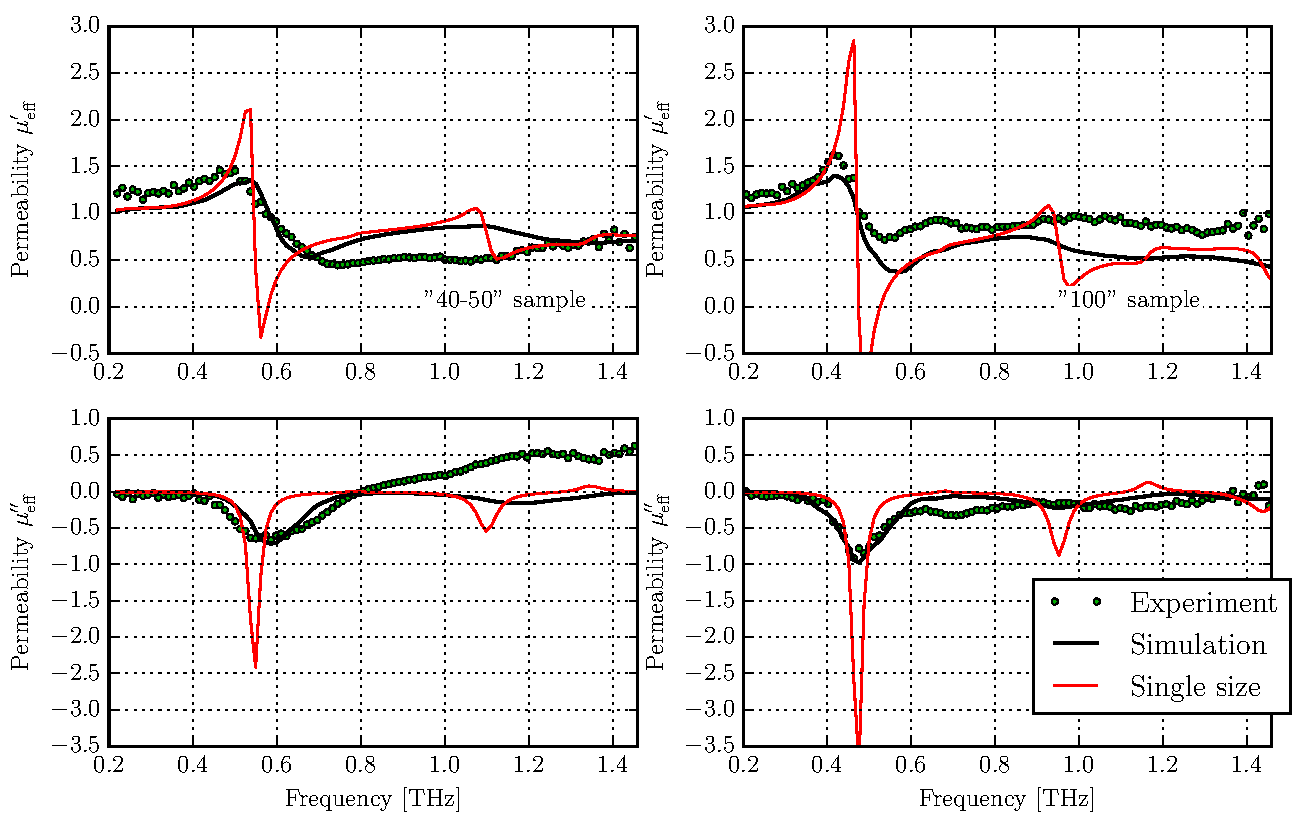
\includegraphics[width=\textwidth]{img-expe/sphere_convolution/mm2012_convolution.pdf}
%/home/sklad/Zalohy/p120528-fzu/p/PhD_TiO2/120118_TiO2_mikrofoto_a_Riadova_simulace
\end{figure}
%}}}
\paragraph{Experimental spectra of spheres} %{{{
We performed series of terahertz time-domain spectroscopy measurements with the titanium microsphere samples. We used the scheme described on pages \pageref{srtm}--\pageref{srtm2} to retrieve not only the transmission of the single-layered sample, but also the effective parameters of a metamaterial the spheres would possibly form when arranged into a lattice. 

The first magnetic Mie resonance was prominent and all retrieved experimental spectra qualitatively conformed to the spectra predicted by FDTD simulations. The quantitative comparison of the results was also possible, but of lesser physical meaning, since two most important quantities, the resonance frequency and the oscillator strength (i.e. amplitude of the resonant waveform) could not be characterised reliably. 

In particular, the exact dielectric permittivity of the polycrystalline rutile was not known, and over the previous years our group established a consensus of $\epsrl' \approx 95$ as in Eq. \ref{eq_tio2}), which provided the best match with most experimental data, and was used and for all related simulations.

Neither the oscillator strength of the first Mie resonance allows for a direct comparison; while it could be determined reliably in the simulations with a given unit-cell size $a$, the exact density of the microspheres was very hard to determine exactly. They were attached to one of the sapphires by static electricity, and their position was random. During any manipulation with such a sample, part of the spheres fell off the sapphire surface. Moreover, we had no reliable way of determining through which part of the sample the probing THz beam passed.

The effective permeability for two samples of different average sphere sizes is represented by dots in Fig. \ref{fg_mm2012_convolution}. The FDTD simulations for an array of identical TiO$_{2}$ spheres yielded much narrower resonant spectra of $\meff(f)$, which are represented by dashed red lines. 

%}}}
\paragraph{Comparison of experimental and simulated spectra}%{{{
To enable a direct comparison, we used the granulometric data obtained by digital processing of the microscopic images. For each sphere, its effective radius $\rho_{\text{eff}}$ was estimated from the major $\rho_1$ and minor axes $\rho_2$ retrieved from the granulometric data for the $m$-th particle: 
\begin{equation} \rho_{\text{eff}}^{(m)} := \left[\frac{1}{3\left(\rho_1^{(m)}\right)^2} + \frac{2}{3\left(\rho_2^{(m)}\right)^2}\right]^{-0.5} \label{eq_rhoconvol}\end{equation}
            %bin_particle_size = (1./3*bin_major**-2 + 1./3*bin_minor**-2 + 1./3*bin_minor**-2)**-.5 
This expression is based on the expectation that the ellipsoids will orient horizontally when sprinkled on the microscope slide, thus making the shortest axis vertical and hidden from the statistical processing. Obviously, it is arbitrary to assume the shortest and medium ellipsoid axis will be both equal to $\rho_2$. 
The correct procedure would be to determine all three axes of the three-dimensional particle and express $\rho_{\text{eff}}$ using Eqs. (\ref{eq_freqM1_rhoxyz}), (\ref{eq_freqE1_rhoxyz}), and similar for higher resonances. It would however require to know all three ellipsoid axes. Changes in these coefficients did not cause a substantial change in the results.

We deduced from the FDTD simulations that the resonance frequency of a TiO$_{2}$ sphere is inversely proportional to its effective radius $\rho_{\text{eff}}^{(m)}$, and its scattering cross-section to the square thereof. Once a reference permeability spectrum $\meff^{\text{(ref)}}(f)$ was computed for a reference radius $\rho^{\text{ref}}$, the experimental spectra could be estimated as the following sum over all $M$ photographed particles:
\begin{equation} \meff^{\text{(simulated)}}(f) := 1 + \frac{\sum\limits_{m=0}^{M} \left[(\rho_{\text{eff}}^{(m)})^{-2} \meff^{\text{(ref)}}\left(\frac{f \rho_{\text{eff}}^{(m)}}{\rho^{\text{ref}} }\right) - 1 \right]}{\sum\limits_{m=0}^{M} (\rho_{\text{eff}}^{(m)})^{-2}}. \label{eq_sumconvol}\end{equation}

	The result, plotted by thick black curves in Fig. \ref{fg_mm2012_convolution}, corresponds to a weighted average through the particle statistics, with the weight proportional to the scattering cross-section of each particle. The averaged simulation results are relatively close to the experimental data at frequencies around the first magnetic Mie resonance (around 600 and 480 GHz, respectively). 
	
	At higher frequencies, the experimental data deviate substantially from the predictions. This can be attributed to one or more sources of imprecision in the experimental setup for effective-parameter retrieval.

			%bin_weight_coef = (bin_particle_size/sim_particle_size)**filling_factor_power 
            %bin_weight = bin_particle_count[n] * bin_weight_coef
            %total_bins_weight += bin_weight

            %## Calculate response of the bin
            %scaled_sim_x = sim_x * (sim_particle_size/bin_particle_size) * (sim_particle_eps/meas_particle_eps)
            %interp_function = interp1d(scaled_sim_x, sim_y, kind='linear', bounds_error=False)
            %bin_response_n = (interp_function(meas_x) - vacuum_property) * bin_weight
            %total_response_n += bin_response_n

            %## Calculate which particle size is the average
            %average_particle_totalsize += bin_particle_size * bin_weight
            %average_particle_totalweight += bin_weight
%}}}
\paragraph{Narrowing the resonance by sieving} %{{{
The broad dispersion of the microsphere sizes leads to broadening of the Mie resonance, in particular it precludes $\meff'(f)$ from reaching negative values, and also it distributes the very strong dissipative losses into all frequencies close to the resonance, including the region where the FDTD simulations in Fig. \ref{fg_Spheres_lossscan} would predict relatively low losses and $\meff'(f) < 0$.

With the aim to resolve this issue which affected all microsphere samples, we developed the novel sieving technique described in the experimental section of this thesis. Fig. \ref{fg_sphere_sieving} compares the independently measured spectra of $\Neff(f)$, $\eeff(f)$ and $\meff(f)$ for three different fractions of one sample. The blue line corresponds to the oversized fraction that remained above the first sieve, the red line to the correctly sized fraction that passed the first sieve but remained above the second one, and the green line to the remaining fraction that passed both sieves.

Moderate narrowing of the resonance spectral shape can be observed for the correctly sized fraction, with the remaining fractions being shifted in the frequency as predicted. The intermediate fraction consistently exhibits more pronounced resonance in the permeability. %The results of the sieving, however, remain inconclusive.
Simultaneously all spectra measured are burdened with one or more severe errors of the characterisation method. Namely in Fig. \ref{fg_sphere_sieving}, the Mie theory can not explain the pronounced resonance in retrieved effective permittivity, which appears as an artifact coming from the asymmetry of the sample between two sapphire plates. This may be also the cause of the spectra of $\eeff(f)$ and $\meff$ usually deviating from the expected values at higher frequencies.

However, the truly fundamental limitation are the dissipative losses in TiO$_{2}$, already shown in Fig. \ref{fg_SphereWire_principles}.  They impose a tight upper bound for the figure of merit of any terahetrz metamaterial based on TiO$_{2}$ resonators. 

%}}}
\begin{figure}[h!] %{{{  fg_sphere_sieving
	\caption{Comparison of retrieved effective parameters for three fractions of a microspheres sample: \textbf{(a)} effective index of refraction, \textbf{(b)} permittivity and \textbf{(c)} permeability. } \label{fg_sphere_sieving} \centering \vspace{-3mm}
\begin{overpic}[width=0.86\textwidth]{img-expe/sphere_sieving/sphere_sieving_n.pdf}\put(-1,38){\textbf{(a)}} \end{overpic}\vspace{-0.046\textwidth}\\
\hspace{1.7mm}\begin{overpic}[width=0.85\textwidth]{img-expe/sphere_sieving/sphere_sieving_eps.pdf}\put(-1,38){\textbf{(b)}} \end{overpic}\vspace{-0.046\textwidth}\\
\begin{overpic}[width=0.86\textwidth]{img-expe/sphere_sieving/sphere_sieving_mu.pdf}\put(-1,38){\textbf{(c)}} \end{overpic}\vspace{-0.036\textwidth}\\
\end{figure}
%}}}
\paragraph{Spheres in a metallic mesh} %{{{
We attempted to fabricate one layer of a metamaterial by embedding resonant particles into the holes of a metallic sieve. This kind of structures is predicted to have a negative index of refraction above the first Mie resonance of the spheres (see the green curve in Fig. \ref{fg_SphereWire_principles}). 

The issues in our case were mostly of geometrical and mechanical origin. Although it was possible to manufacture a sieve with proper size of holes which would hold microspheres during sieving, the spheres randomly fell out of it upon manipulation. We decided not to use any glue, since even a relatively thin layer thereof would substantially alter the spectra, possibly dramatically increasing losses in the terahertz range.

An experiment involving a similar sample was published previously \cite{yakiyama2012terahertz}, with TiO$_{2}$ spheres sprinkled over a commercial mesh woven of steel wire, as sketched and accurately measured in Fig. \ref{fg_spherewire_sketch}b,d. The original publication reported very low transmission, with inconclusive result as regards to the negative phase advance through the structure. This structure is asymmetric, with $\Delta z$ estimated to $15$ $\upmu$m from geometrical reasons, and thus the effective parameter retrieval yields unphysical values.

% todo add some links to Zhao etc.?
%}}}
%   SKIP  \begin{figure}[h] \caption{Current-driven homogenization results for TiO$_2$ spheres %{{{
%    \textbf{(a)} without wires and  \textbf{(b)} embedded in a wire mesh.} \label{fg_cdh3} \centering 
%    	\begin{overpic}[width=.48\textwidth]{img-cdh/cdh_SpheresTiO2.pdf}  \put(1,96) {\textbf{(a)}} \end{overpic}
%    	\begin{overpic}[width=.48\textwidth]{img-cdh/cdh_SpheresLossLess.pdf}  \put(1,96) {\textbf{(b)}} \end{overpic}
%    \end{figure}
%    
%    %}}}
%   SKIP \paragraph{Tunable dielectric resonators} %{{{
% todo "At low temperatures, ε approaches a limiting value of 257 in the c direction and 111 in the a direction. ε300°K=170 and 86, respectively, and ε1000°K=97 and 58. " -- Parker R. A. Static dielectric constant of rutile (TiO2), 1.6-1060 K



%   %TODO Note that the effect of mm-phc transition can be also observed in silicon microcubes (thz operation)
%   %Planar all-silicon metamaterial for terahertz applications \cite{prosvirnin2015planar}
%   
%   %}}}
\FloatBarrier %====================================================================================================
%}}}
\section{Dielectric rods parallel to the magnetic field} % TODO review%{{{
\paragraph{Resonances in a low-permittivity array}	\label{sect_diel_rods_mag}	%{{{
Dielectric rods aligned parallel to the magnetic field exhibit spectra similar to the sphere arrays (see Fig. \ref{fg_rodsphere_comparison}), with clearly identifiable Mie resonances with magnetic and electric dipoles.
Unlike sphere arrays, the computation of the rod array behaviour under near-perpendicular incidence is a two-dimensional problem. 

Photonic crystals composed of dielectric rods in a square lattice have been examined thoroughly since early 1990s \cite{plihal1991two, pendry1992_transfer_matrix}. The permittivity of the constituent materials was usually rather low, typically up to the permittivity of silicon $\varepsilon \leq 12$, assuming the structure would operate at optical or near-infrared frequencies. 

In the left panel of Fig. \ref{fg_rodh}, the relatively low permittivity in the structure causes its low-frequency behaviour to be similar to the one-dimensional photonic crystal. At the lower edge of the Bragg band gap ($X1$ subplot of \ref{fg_rodh}a), the electromagnetic wave concentrates the electric field in the layer of dielectric rods, as indicated by tiny arrows. The magnetic field energy is roughly complementary, located predominantly in the air between them. As already described on the example of 1-D PhC, the upper edge of the band reverts the situation. The number of nodal planes of the electric or magnetic field does not change between the lower and upper edges of a Bragg band gap.

%}}}
\begin{figure}[ht] %{{{ rodsphere_comparison
	\caption{Comparison of \textbf{(a)} transmittance and \textbf{(b)}  effective index of refraction $\Neff$ for arrays of dielectric spheres (with radius $\rho_s=30$ $\mu$m) and of dielectric rods (with radius $\rho_r=19$ $\mu$m) in a 100 $\upmu$m unit cell, both made of TiO$_2$. The choice of radii used ensures the same volume filling fraction. } \label{fg_rodsphere_comparison} \centering \vspace{-3mm}
\begin{tabular}{r}
\begin{overpic}[width=0.95\textwidth]{img-meep/rodsphere_comparison_t.pdf} \put (-1,27) {\textbf{(a)}} \end{overpic}\vspace{-0.055\textwidth}\\
\begin{overpic}[width=0.96\textwidth]{img-meep/rodsphere_comparison_n.pdf} \put (-1,27) {\textbf{(b)}} \end{overpic}\vspace{-0.\textwidth}\\
\end{tabular}
\end{figure}
%}}}
\paragraph{Resonances in the high-permittivity array} %{{{
In the microwave and terahertz ranges, the permittivity of many materials turns out to be much higher than 12. This fact gives rise to the main difference between the panels in Fig. \ref{fg_rodh}. In the right panel, the dielectric permittivity $\epsrl=100$ moves the first Mie resonance \cite{obrien2002photonic} in the first band gap. 

This band gap starts in the $X1$ point, where each unit cell is divided by one nodal plane of the magnetic field. In contrast, the next photonic band starts in the $\Gamma2$ point where no such nodal plane exists. This corresponds to a drop in the real part of effective index of refraction, a behaviour that is typical for all individual resonances.

%\textit{magnetic Mie resonance}, \cite{obrien2002photonic, nemec2009tunable, yahiaoui2009broadband, yahiaoui2011tunable}

%}}}
\begin{figure}[ht]  %{{{ fg_rodh
	\caption{Dispersion curves for an array of dielectric rods parallel to the magnetic field. The side plots show the shapes of the fields in the $(x,z)$ plane, at the frequencies of the band edges. The magnetic field is plotted as orange-violet color map and the electric field is represented by vectors. The rod radius was chosen to 12 \% of the period. \textbf{(a)} On the left, a relatively low permittivity $\epsrl = 12$ places the magnetic resonance above the first Bragg band gap. \textbf{(b)} For high permittivity dielectric $\epsrl = 100$, the magnetic resonance forms the first band gap. } \label{fg_rodh} \centering
\begin{overpic}[width=.48\textwidth]{img/HRods_eps012_R12_PWEM.pdf}\put(1,96) {\textbf{(a)}} 
\put(0,1){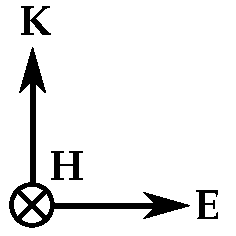
\includegraphics[width=.12\textwidth]{img/tripletKHE.pdf}}
\end{overpic}
\begin{overpic}[width=.48\textwidth]{img/HRods_eps100_R12_PWEM.pdf}\put(1,96) {\textbf{(b)}} \end{overpic}
\end{figure}
%}}}
%SKIP \begin{figure}[ht]  \caption{Effective parameters of an array of dielectric rods $||\mathbf H$ with same parameters as in Fig. \ref{fg_rodh}b (i.e. radius of  12 \% of the period and permittivity $\varepsilon = 100$). Complex reflection $r$ and transmission $t$ spectra allow to compute the effective index of refraction, impedance (not shown), permittivity and permeability. Thin black lines indicate the Brillouin zone boundaries.}%{{{
%\label{fg_rodh_fdtd} \centering 
%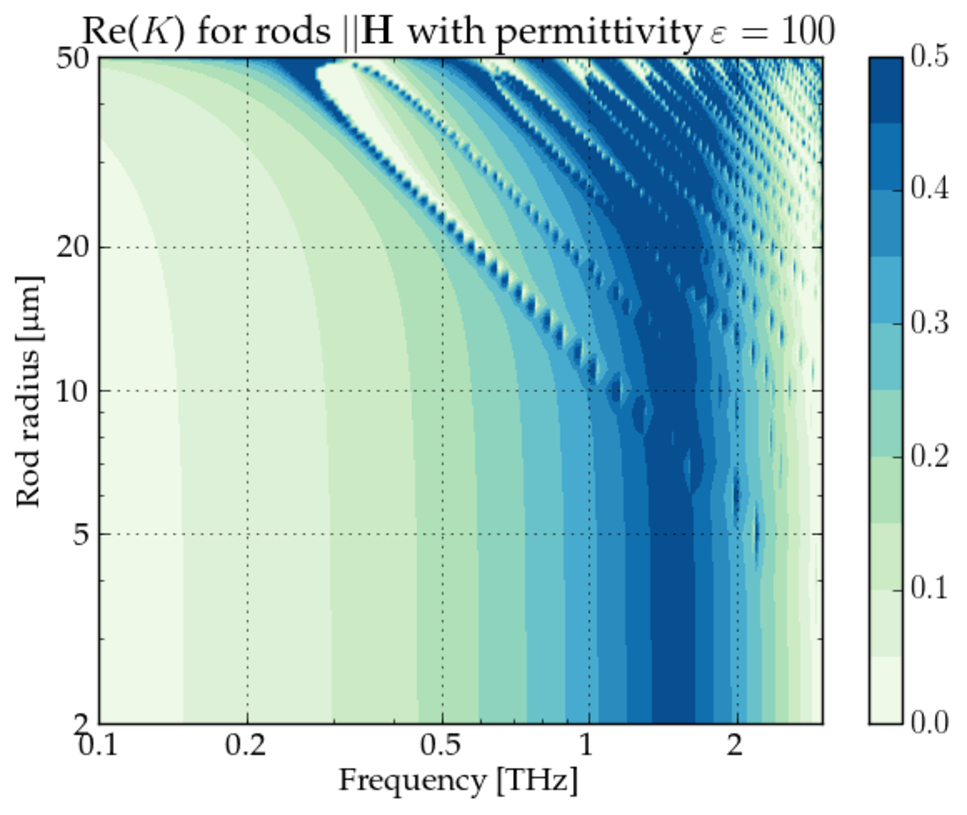
\includegraphics[width=8cm]{img/old/HRods_eps100_radiusscan.pdf}
%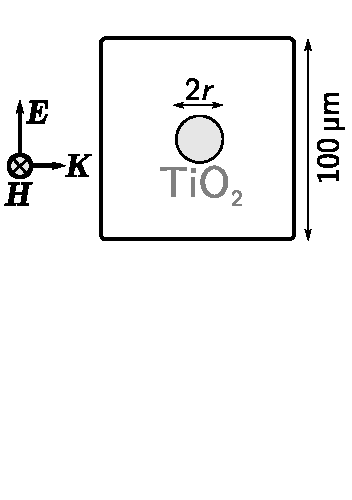
\includegraphics[width=4.5cm]{img/HRods_sketch.pdf}
%\end{figure}
%}}}
%\begin{figure}[ht] \caption{The spectra of the wavenumber $K$ for different rod radii and two different rod permittivities. The wavenumber plot is folded so it ranges from 0 to 0.5, where $K\approx 0$ and $K\approx 0.5$ correspond to band gaps. \textbf{(a)} Medium-permittivity rods with $\varepsilon = 12$, \textbf{(b)} high-permittivity rods with $\varepsilon = 100$.  } \label{fg_hbar_radiusscan} \centering %{{{
%\textbf{(a)}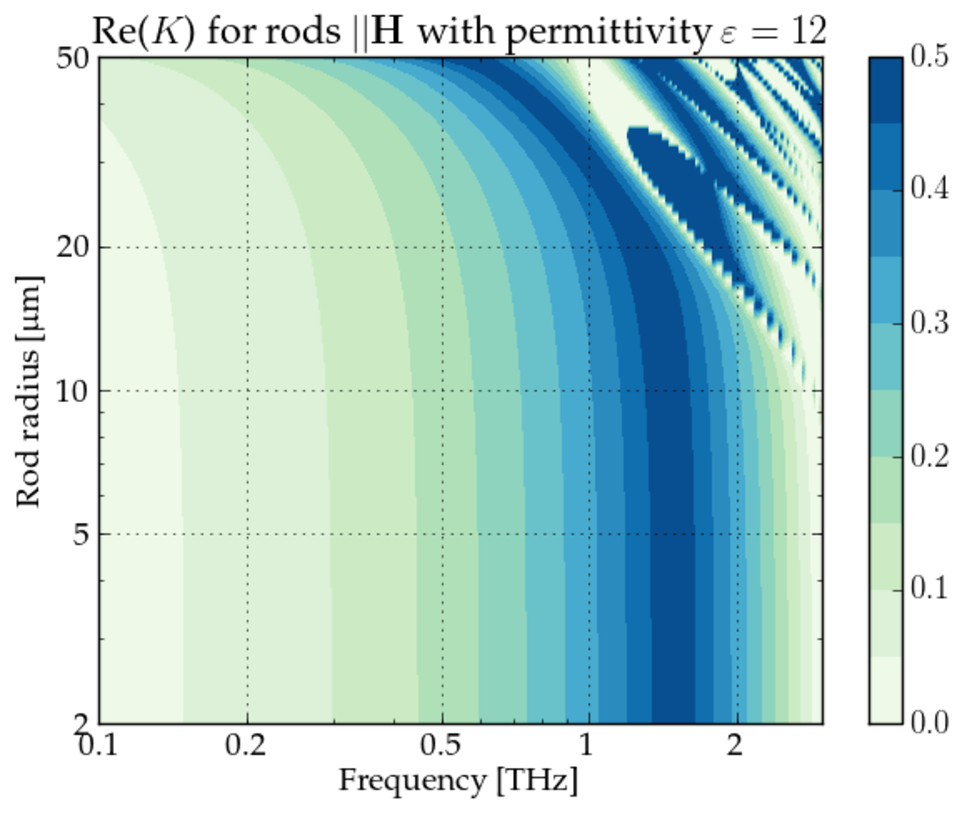
\includegraphics[width=8cm]{img/old/HRods_eps012_radiusscan.pdf}
%\textbf{(b)}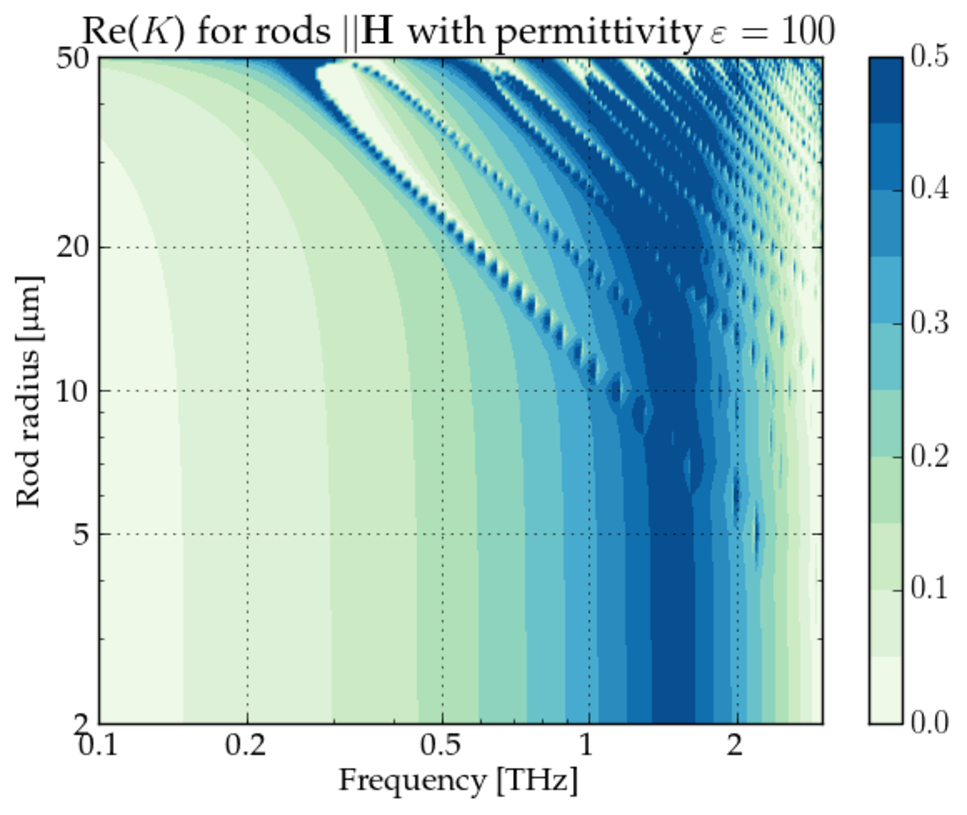
\includegraphics[width=8cm]{img/old/HRods_eps100_radiusscan.pdf}
%\end{figure}
%}}}
\FloatBarrier %====================================================================================================
%}}}
\section{Dielectric rods parallel to the electric field} \label{sect_diel_rods_el} %{{{
\begin{figure}[h!]  %{{{ erods_acomparison
	\caption{Amplitude of \textbf{(a)}  reflectance, \textbf{(b)} transmittance \textbf{(c)} effective index of refraction $\Neff$ and \textbf{(d)} effective permittivity $\eeff$ for a rod array with constant radius $\rho = 10$ $\mu$m, dielectric permittivity  and grid resolution of 1 $\mu$m. } \label{fg_erods_acomparison} \centering \vspace{-3mm} 
%% NOTE: if realistic materials are needed, erods_acomparison-loLoss_r.pdf can be substituted for  erods_acomparison_r.pdf etc.
\begin{tabular}{r}
\begin{overpic}[width=0.85\textwidth]{img-meep/erods_acomparison-loLoss_r.pdf} \put (-1,28) {\textbf{(a)}} \end{overpic}\vspace{-0.060\textwidth}\\ 
\begin{overpic}[width=0.85\textwidth]{img-meep/erods_acomparison-loLoss_t.pdf} \put (-1,28) {\textbf{(b)}} \end{overpic}\vspace{-0.057\textwidth}\\
\begin{overpic}[width=0.85\textwidth]{img-meep/erods_acomparison-loLoss_n.pdf} \put (-1,28) {\textbf{(c)}} \end{overpic}\vspace{-0.055\textwidth}\\
\begin{overpic}[width=0.85\textwidth]{img-meep/erods_acomparison-loLoss_eps.pdf} \put (-1,28) {\textbf{(d)}} \end{overpic}\vspace{-0.030\textwidth}\\
\begin{overpic}[width=0.85\textwidth]{img-meep/erods_acomparison-loLoss_mu.pdf} \put (-1,28) {\textbf{(e)}} \end{overpic}\vspace{-0.030\textwidth}\\
\end{tabular}
\end{figure}
%}}}
\paragraph{Sparse rod array} %{{{
The discussion of the previous structure has proven that the choice of permittivity and geometry obviously leads to a qualitative change in the structure behaviour. This becomes even more important in the case of dielectric rods parallel to the electric field. 

Fig. \ref{fg_erods_acomparison} shows the spectra of effective parameters for three rod arrays of the same permittivity $\epsrl(f=1\text{ THz}) = 89.5+0.23\ii$ and diameter $\rho=10$ $\upmu$m. They only differ by the unit cell size $a \in \{80, 90, 120\}$ $\upmu$m, yet such a structure obviously behaves in several different ways depending on $a$. Moreover, the differences are not obvious if PWEM results are plotted, as was the case in Fig. \ref{fg_rodh}.  

% TODO refereence  also to \cite{valdivia2012} and \cite{shi2007}
%low-loss dielectrics discussed in http://www.nature.com/nnano/journal/v11/n1/full/nnano.2015.304.html??
%\cite{yang2015}
Starting with the blue curves in Fig. \ref{fg_erods_acomparison} representing a sparse array with $a=12\rho = 120$ $\upmu$m, one can clearly identify two individual resonances around 745 and 1170 GHz, each introducing a familiar shape in the spectra of $\Neff(f)$. From the effective permittivity $\eeff(f)$ and permeability $\meff(f)$, the first resonance can be identified as an electric one, and the second as a magnetic one. The electric resonance has a strong dipole moment and introduces a broader band gap than any of resonances shown in Fig. \ref{fg_rodsphere_comparison}. %; the fundamental asymmetry arises from the fact that the spheres and rods are made of a dielectric that primarily interacts with the electric field, while its permeability $\murl=1$. 

In spite of the strength of the first resonance, the corresponding region of $\eeff'(f)<0$ does not overlap with that of $\meff'(f)<0$ for the sparse rod array with $a=120$ $\upmu$m and no negative index of refraction is obtained. The resulting spectra of all parameters are qualitatively similar to that of the electro-magnetic resonator with the capacitor radius $\rho_c\gtrsim 18$ $\upmu$m  (c.f. Figs. \ref{fg_emSRR_icr} and \ref{fg_cdh2}b).

%}}}
\paragraph{Effect of inter-cell coupling}%{{{
By increasing the filling fraction of the dielectric rod, the electric and magnetic resonances can be efficiently tuned upwards and downwards in the frequency, respectively. 
The reason can be traced down to the symmetry of the magnetic field shapes. 

The electric resonance (Fig. \ref{fg_sketchfield}a), with the electric dipole pointing parallel to the rod, and the magnetic field circulating around it, introduce opposite orientation of the magnetic field at the cell boundaries. Reduction of the cell size $a$ also reduces the effective inductance of the rod per unit length, thus shifting the electric resonance upwards.

On the contrary, the magnetic field surrounding the rod near the magnetic Mie resonance (Fig. \ref{fg_sketchfield}b) has the same orientation at the cell boundaries as that of the neighbouring cell. Thus the reduction of $a$ and reduces the frequency of the magnetic resonance.

Note that this strong coupling is specific for this particular rod orientation. In the previous chapter we discussed similar high-permittivity rods oriented parallel to the magnetic field. In the first resonance, the electric field circulated around the rod axis, but taking into account that the electric field energy density is proportional to $\epsrl$, majority of its energy was confined to the dielectric volume (cf. Fig.  \ref{fg_hrod}b-$\text{X}1$).  The inter-cell coupling of the magnetic resonance was thus much weaker, and similar argument applies to all higher resonances. As a result, the resonance frequencies of dielectric rods parallel to the magnetic field can not be tuned against each other as in the case of rods parallel to the electric field.

%}}}
\begin{figure}  %fg_sketchfield%{{{
\caption{Cross-sections of first two resonant modes in the dielectric rod. The red and blue color shows positive and negative values of the electric field, while the magnetic field is represented by the arrows. \textbf{(a)} The electric Mie resonance, \textbf{(b)} the magnetic Mie resonance.} \label{fg_sketchfield} \centering 
\begin{overpic}[width=.8\textwidth]{img/ERods_1st_and_2nd_Mie_resonance.pdf} \put(10,29.2) {\textbf{(a)}} \put(45,29.2) {\textbf{(b)}} 
\put(85,8){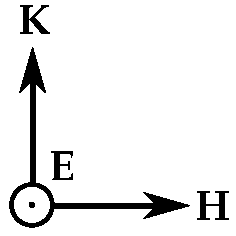
\includegraphics[width=.12\textwidth]{img/tripletKEH.pdf}}
\end{overpic}
\end{figure}
%}}}
\begin{figure}[ht] %{{{fg_erod_radius11 PWEM TODO
\caption{Behaviour of the rods $||\mathbf E$, with permittivity $\varepsilon = 100$ and radius $r=11\;\upmu$m.} \label{fg_erod_radius11} \centering 
\begin{overpic}[width=.48\textwidth]{img/ERods_eps100_R11_PWEM.pdf}\put(1,96) {\textbf{(a)}} 
\put(0,1){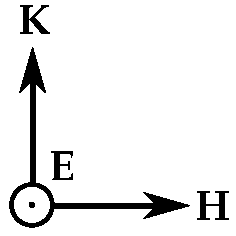
\includegraphics[width=.12\textwidth]{img/tripletKEH.pdf}}
\end{overpic}
%  \begin{figure} \caption{img/ERods\_eps100\_single\_a120\_FDTD.pdf}  \centering 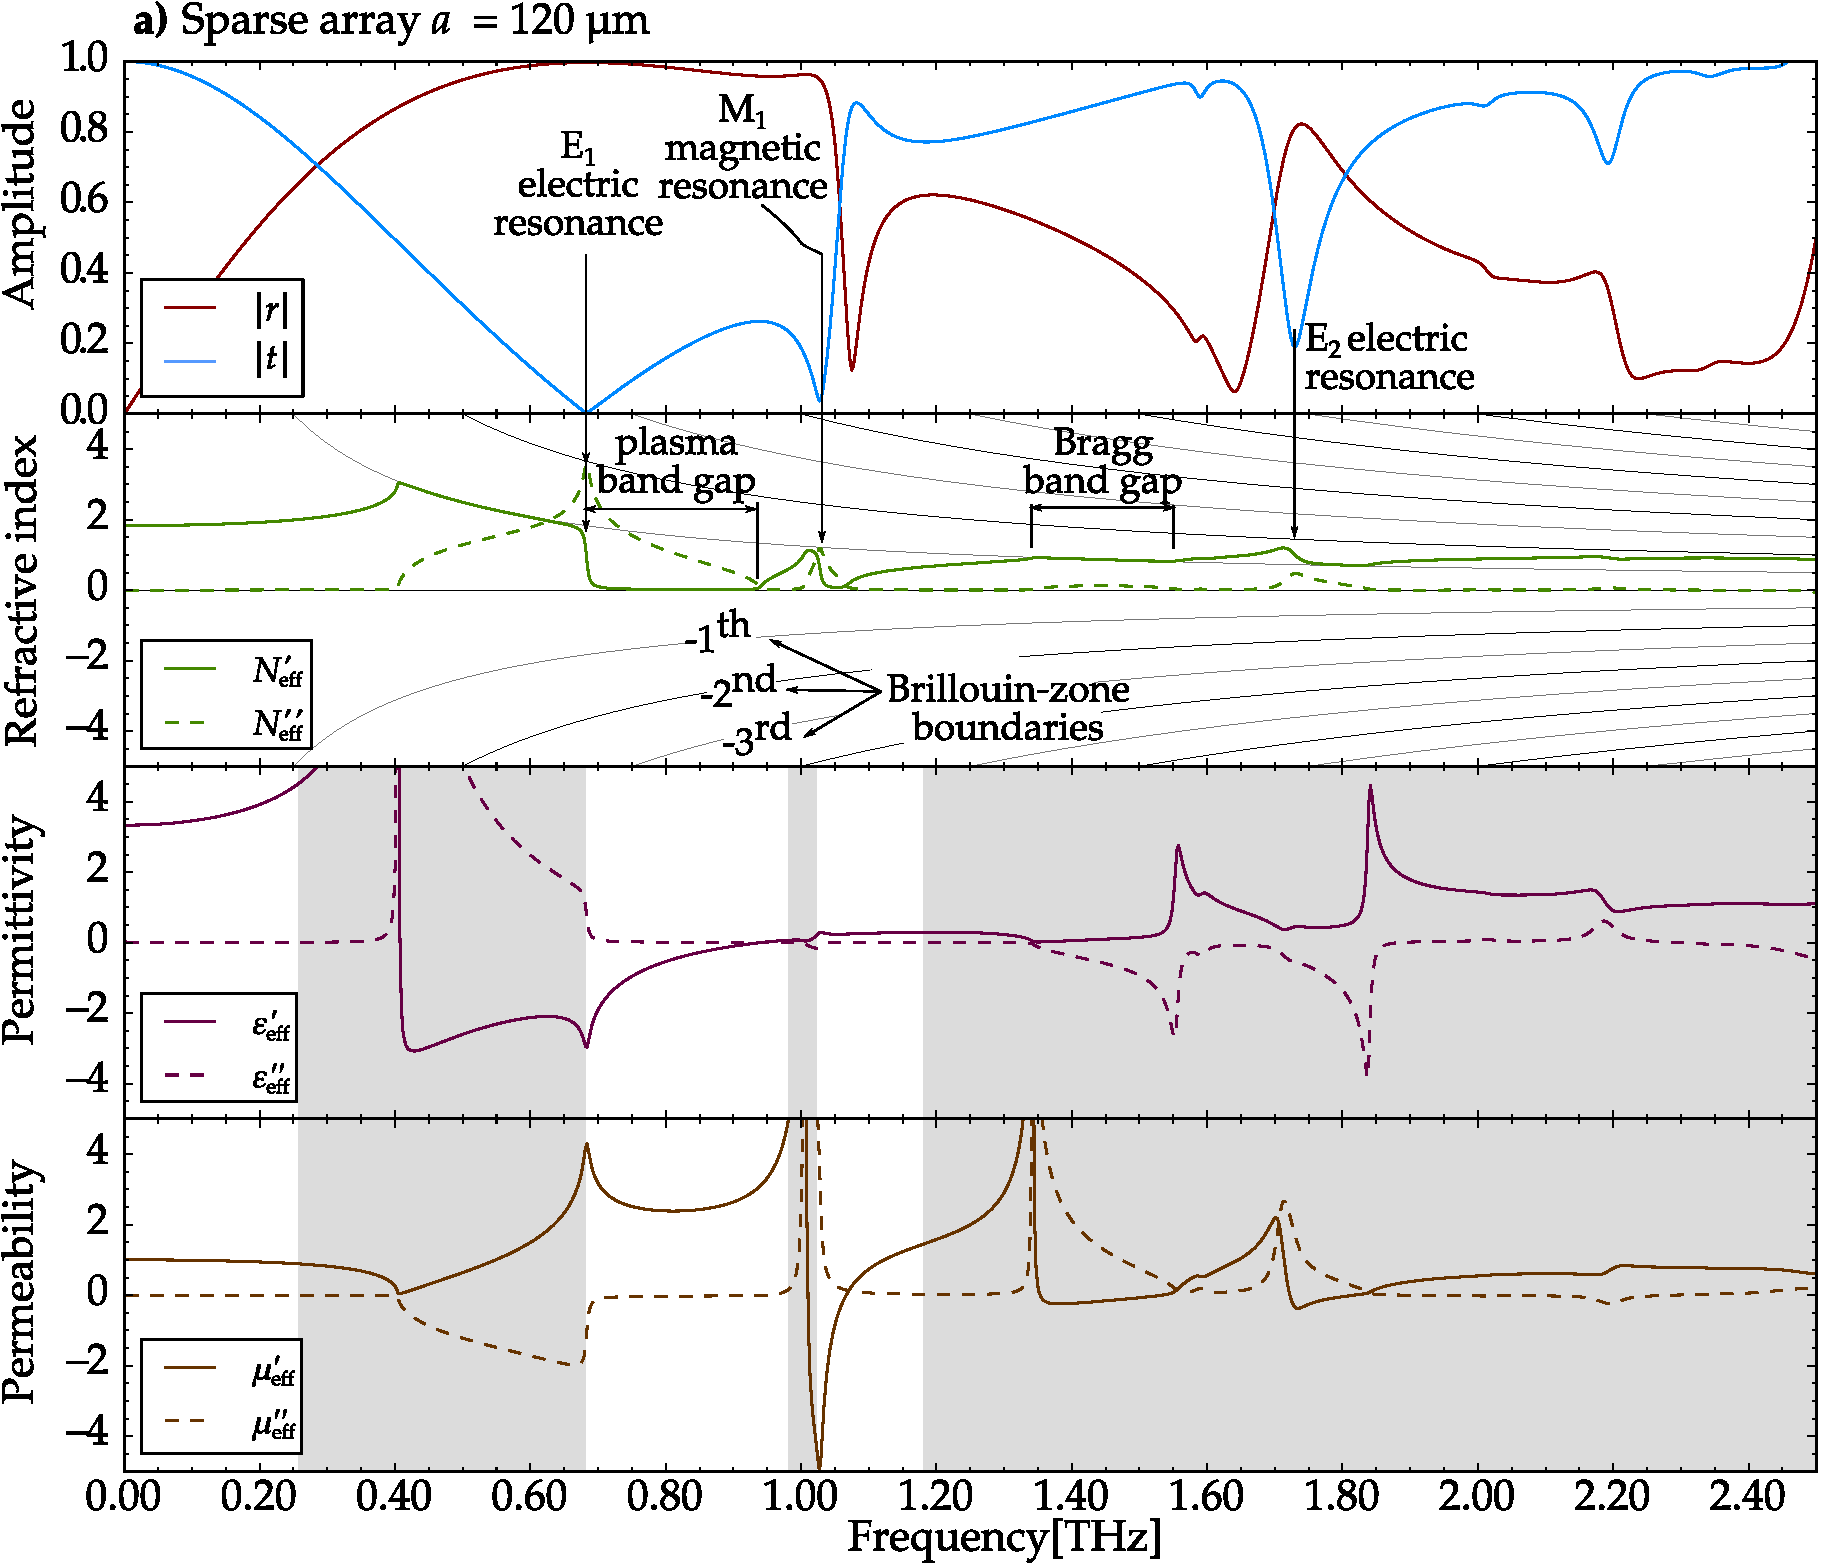
\includegraphics[width=10cm]{img/ERods_eps100_single_a120_FDTD.pdf} \end{figure} 
%  \begin{figure} \caption{img/ERods\_eps100\_triple\_a150a100a080\_FDTD.pdf}  \centering 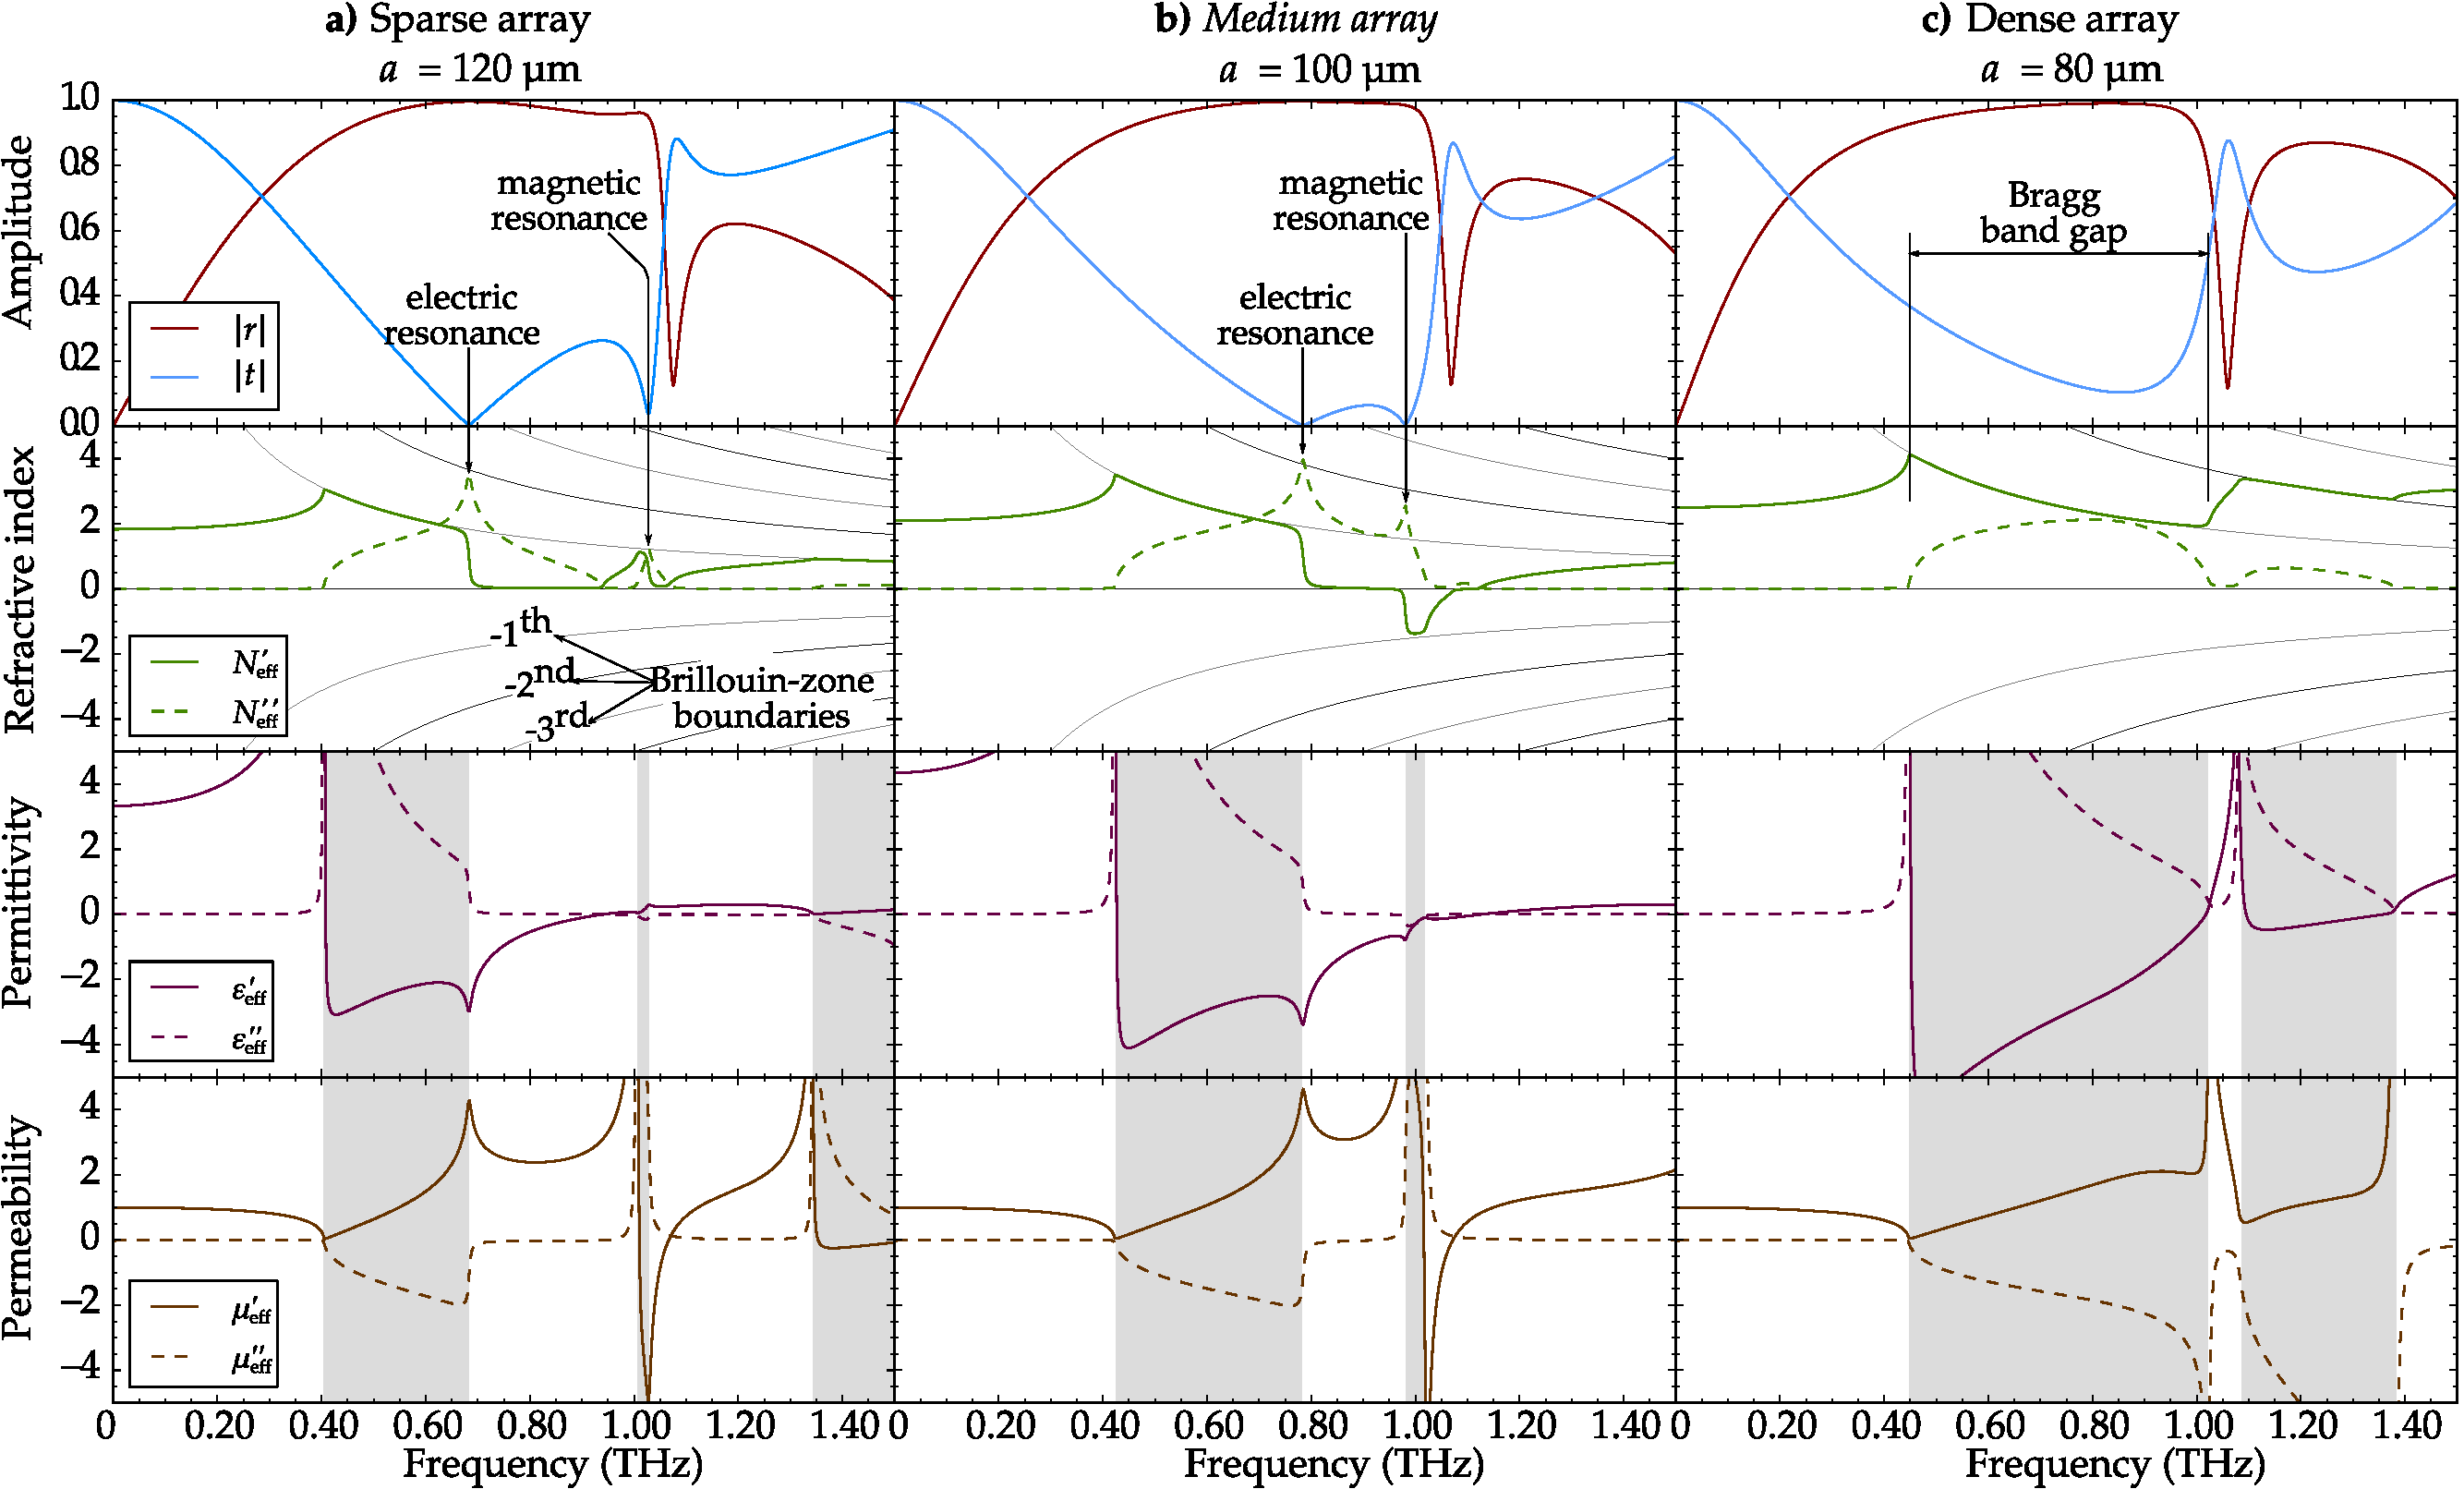
\includegraphics[width=10cm]{img/ERods_eps100_triple_a150a100a080_FDTD.pdf} \end{figure} 
%  \begin{figure} \caption{img/ERods\_forSeefeld\_sparserN\_denserN\_DrawnBands.pdf}  \centering 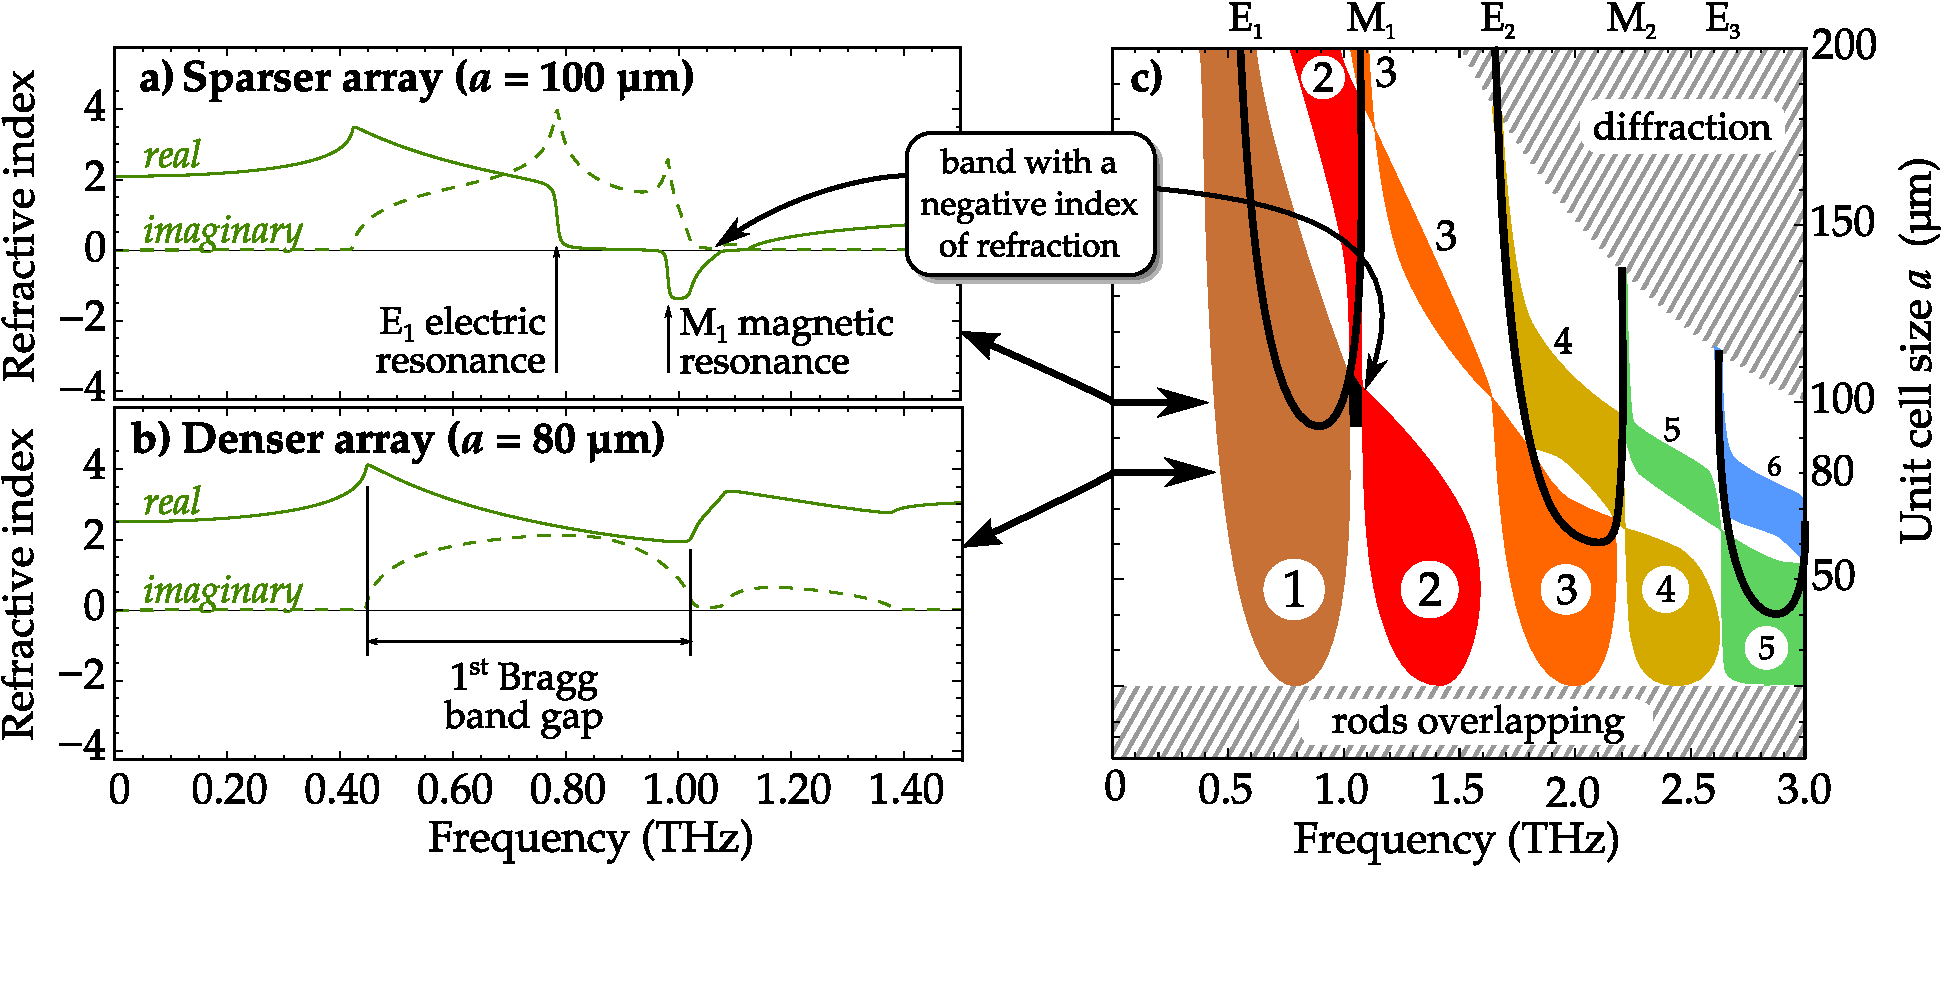
\includegraphics[width=10cm]{img/ERods_forSeefeld_sparserN_denserN_DrawnBands.pdf} \end{figure} 
\end{figure}
%}}}
\paragraph{Medium-density rod array}%{{{
Through moderate reduction of the unit cell size $a$ to 90 $\upmu$m, as represented by the green line in Fig. \ref{fg_erods_acomparison}, the electric and magnetic resonance frequencies approach each other, shifting to $f_E \approx$ 950 and $f_M \approx$ 1070 GHz, respectively. This eventually leads to an overlap of the $\eeff'(f)<0$ and $\meff'(f)<0$ regions, and a negative-index band is formed between 1130 and 1200~GHz.  

At the upper-frequency edge of the band with $\Neff'<0$, either the effective permeability or permittivity becomes positive, for $a\lesssim 92$ $\upmu$m or  $a\gtrsim 92$ $\upmu$m, respectively. This is another subtle, but qualitative change in the structure behaviour. 
%It manifests itself in the mode shapes resolved by PWEM, and the effective impedance $\Zeff=\sqrt{\meff/\eeff}$ reaching either very low or very high values at the band edge. 
At the exact radius of cross-over, the effective permittivity and permeability change their sign at the same frequency, and a \textit{zero-width band gap} is obtained. Unlike the Fabry-Pérot resonances in 1-D PhC, this band gap is located at $\Neff'=0$, which results in a peculiar regime of operation: In an idealized loss-less model, the wave does not exponentially decay nor acquires any phase advance in the metamaterial volume. Still, its group velocity is nonzero. Hence, a spatial modulation of the wave envelope can propagate over the wave, which oscillates in phase. This can be viewed as a complementary phenomenon to the narrow photonic bands, where, due to vanishing inter-cell coupling, the phase velocity is orders of magnitude higher than the group velocity (c.f. the second band in Fig. \ref{fg_cdh2}b).

Both points of near-zero transmittance at $f_E$ and $f_M$, indicating individual resonances, come closer to each other with further reduction of $a$. The maximum transmittance between both resonances decreases approximately with the second power of the frequency difference:
\begin{equation} \underset{f \in\,\langle f_E,f_M\rangle}{\text{max}} |t| \propto \frac{1}{(f_E-f_M)^{2}}, \label{eq_fEfM}\end{equation}
hence the transmitted energy drops with the fourth power of the resonance frequency difference, $f_E-f_M$, and reaches extremely low values. Simultaneously, the transmittance grows above $f_M$ and reaches almost 100 \% relatively close to this low-transmittance region. 
We proposed \cite{dominec2014transition} that with the aforementioned geometry, a single layer of unit cells could find its application as a \textit{dielectric-rod array filter}. It would possess better extinction ratio than a dielectric slab of similar material can achieve through Fabry-Pérot resonances.
% (see Fig. \ref{fg_Slab_fillfraction015_epsilon_comparison})

%}}}
\begin{figure}[htb] %{{{ fg_spacingscan100
	\caption{\textbf{(a)} Reflectance, \textbf{(b)} transmittance, \textbf{(c)} the real and \textbf{(d)} the imaginary part of the retrieved refractive index of an array of dielectric rods made of TiO$_{2}$, with a constant radius $\rho = 10$ $\upmu$m and a variable unit cell size $20\:\mu$m $<a<200\:\mu$m.  Three selected values of radius, discussed in the text, are marked by horizontal black dash-dotted lines.} \label{fg_spacingscan100}  \centering
\begin{overpic}[width=0.48\textwidth]{img-meep/erods_ascan-loLoss_r.pdf}\put(-1,80){\textbf{(a)}}\end{overpic}
\begin{overpic}[width=0.48\textwidth]{img-meep/erods_ascan-loLoss_t.pdf}\put(-1,80){\textbf{(b)}}\end{overpic}\\
\begin{overpic}[width=0.48\textwidth]{img-meep/erods_ascan-loLoss_nr.pdf}\put(-1,80){\textbf{(c)}}\end{overpic}
\begin{overpic}[width=0.48\textwidth]{img-meep/erods_ascan-loLoss_ni.pdf}\put(-1,80){\textbf{(d)}}\end{overpic}
\end{figure}
%}}}
\paragraph{Dense rod array} %{{{
Further reduction of the unit cell size $a$ to 80 $\upmu$m does not lead to a cross-over of the resonance frequencies, as might be expected. Instead, the individual resonances disappear, and an ordinary Bragg band gap remains, spanning from 480 to 1150~GHz. The corresponding transmittance curve  (plot in red in Fig. \ref{fg_erods_acomparison}b) does not touch zero anywhere in the spectrum. 

Consequently, there is no fast drop of $\Neff'(f)$ (see Fig. \ref{fg_erods_acomparison}c). The effective index of refraction $\Neff'$ maintains high values over whole spectrum, which precludes to describe the structure as a homogeneous one. Thence, the local effective parameters of permittivity and permeability cease to have physically useful values anywhere above the middle of the first photonic band.
This kind of behaviour was already encountered in the spectra of one-dimensional photonic crystal (Figs. \ref{fg_Slab_fillfraction015_epsilon_comparison}, \ref{fg_Slab_fillfraction015_epsilon_comparison}). 

However, the effective index of refraction $\Neff(f)$ is still valid, and its spectrum for $a=80$ $\upmu$m still maintains the shape that $\Neff'$ had for $a=90$ $\upmu$m and even $a=120$ $\upmu$m: Most notably, the negative-index band around 1200 GHz, spanning between the -1th and the 0th Brillouin-zone boundaries) on the green curve has its analogy in a similarly narrow band on the red curve (between the 1th to the 2nd Brillouin-zone boundaries). Also the higher frequency features tend to be similar. This suggests that the only qualitative change between $a=90$ $\upmu$m and $a=80$ $\upmu$m is in \textit{the wave phase} per unit cell.

%}}}
\begin{figure}%{{{ fg_drawn100
  \begin{minipage}[c]{0.48\textwidth}
\hfill
	\begin{overpic}[width=\textwidth]{img/erods-ascan_drawn.pdf}
	\put(102,2){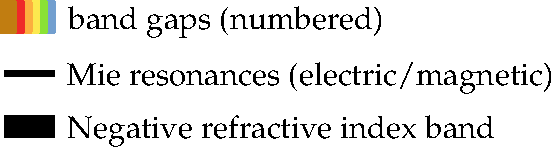
\includegraphics[width=.8\textwidth]{img/erods-ascan_legend.pdf}}
	\end{overpic}
  \end{minipage}
  \begin{minipage}[c]{0.5\textwidth}
    \caption{Scheme of band gaps and Mie resonances under the same conditions as in Fig.~\ref{fg_spacingscan100}. 
In the upper-right corner of the plots, for $a>c/f$, an empty area is left where the diffraction precludes determination of effective parameters.\\
The colours and numbering from 1 to 6 denote the band gaps. Mie resonances are outlined by thick black curves. A small black patch close to the center of the figure depicts the conditions of negative index of refraction. \vspace{18mm}  } \label{fg_drawn100}
  \end{minipage}
\end{figure}

%}}}
\paragraph{Continuous scan through the unit cell sizes}%{{{
For illustration, we add a high-resolution continuous scan through the unit cell size $a$ in Fig. \ref{fg_spacingscan100}, with other parameters shared with the previous plots in Fig. \ref{fg_erods_acomparison}. The individual Mie resonances can be identified as the sets of points where transmittance $|t|$ comes close to zero, real part of effective index of refraction $\Neff'$ drops and its imaginary part $\Neff''$ has a sharp peak. The photonic band gaps are all areas where $\Neff'' \not\approx 0$ in Fig. \ref{fg_spacingscan100}d.

For easier interpretation, the interplay of the individual resonances and the band gaps is redrawn in Fig. \ref{fg_drawn100}, where each photonic band gap is represented as a coloured area and the individual resonances as thick black lines. The small black patch between the first and second band gaps covers the range conditions necessary for reaching $\Neff'<0$, provided that the dielectric is titanium dioxide with permittivity $\epsrl \approx 92$. 

Related effects were described in the literature. Ref. \cite{shi2007} investigates the impact of Mie resonances to the band-gap structure, but the discussion thereof neglects the near-field effect on Mie resonance frequency. The paper unfortunately did not include refined scans of the $a/\rho$ ratio and thus did not correctly discuss the qualitative change in the structure behaviour. 

In accordance with the previous discussion, the electric and magnetic Mie resonances approach each other when the unit cell size $a$ decreases from 120 to 90 $\upmu$m, and eventually they meet and vanish for $a \lesssim 85$ $\upmu$m, forming an "U"-shaped curve. Using $a$ as the scanning parameter enables to clearly illustrate the shift of individual resonances. With this choice, the frequencies of the band gaps roughly follow the $1/a$ curves, but they are strongly influenced by the individual resonances. Each individual resonance is always contained inside a band gap.

In photonic bands, the real part of refractive index grows as a function of frequency; from the beginning to the end of each photonic band, it gains a difference of one Brillouin zone. The only way how $\Neff'$ can descend by one Brillouin-zone boundary is by means of an individual resonance. A simple arithmetic rule for reaching negative index of refraction $\Neff'(f_1)<0$, at a given frequency $f_1$, is therefore that the number of photonic band gaps counted from $f=0$ to $f_1$ must be strictly less than the number of individual resonances. 
%(Author conjectures that the presence of two Mie resonances in the \textit{first} band gap in the spectrum is a necessary and sufficient condition for $\Neff'<0$ to occur.)
This simple rule eliminates the possibility of obtaining $\Neff'<0$ from any higher-order Mie resonances, although they can be shown to persist for smaller unit cell sizes than $a=85$ $\upmu$.  (Figs. \ref{fg_spacingscan100}, \ref{fg_drawn100})

%}}}
\begin{figure}[t] % fg_fxplot %{{{
\begin{minipage}[c]{0.51\textwidth}
	\hspace{-2mm}\begin{overpic}[width=.99\textwidth]{img-meep/erods_fxplot_cs120e-6.pdf} 
		\put(117,8){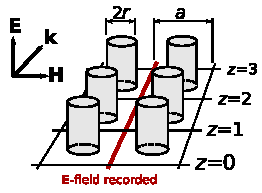
\includegraphics[width=.5\textwidth]{img/ERods_sketch_recordedline.pdf}}
		\put(7,90) {\textbf{(a)}} 
	\end{overpic}\\
\end{minipage}
\begin{minipage}[c]{0.49\textwidth}
	\caption{Spatially resolved spectra of the electric field for the unit cell cell sizes \textbf{(a)} $a=120$ $\upmu$m and \textbf{(b)} $a=90$ $\upmu$m \textbf{(c)} $a=80$ $\upmu$m  }\vspace{3cm} \label{fg_fxplot}
\end{minipage}  
%\vspace{-12mm}
%\end{figure} 
%\begin{figure}[h!] 
\hspace{-2mm}\begin{overpic}[width=.51\textwidth]{img-meep/erods_fxplot_cs90e-6.pdf}  
	\put(7,90) {\textbf{(b)}} 
\end{overpic}
\hspace{-1mm}\begin{overpic}[width=.51\textwidth]{img-meep/erods_fxplot_cs80e-6.pdf}  
	\put(7,90) {\textbf{(c)}} 
\end{overpic}
\end{figure} 
%}}}
\paragraph{Inspection of the frequency-dependent shape of the field}%{{{
While the PWEM plot gives full information about the field at the band edges (Fig. \ref{fg_erod_radius11}), it does not compute the field shape at frequencies lying in the band gap, which is exactly what we need to explain the physical reason behind the peculiar disappearance of Mie resonances. Inspection the fields within a band gap requires a new kind of plots based on time-domain simulations, which show how the electric field amplitude depends simultaneously on the position along the wave vector, i.e., the $z$-axis, and on the frequency (Fig. \ref{fg_fxplot}). 
%, since the wave amplitude decays exponentially and the field is not eigenfunction of the  

A structure of dielectric rods arranged in three layers was used as a sufficiently thick sample to illustrate the metamaterial behaviour. Since the discussion is based on the phase advance of the wave across a cell, it is sufficient to observe the fields at the central line between the rods only (see drawing in \ref{fg_fxplot}).

The electric field amplitude was stored in each simulation step for each point along the line.
At the end of the simulation, the temporal spectra of the record were computed and the magnitude of $|E_x(z, f)|$ was plotted. A logarithmic color map spanning over 5 orders of magnitude was used, with dark blue representing lowest field magnitude and white highest. For easier comparison, the effective index of refraction was added below each plot of the fields, with a shared frequency axis.
To the author's knowledge, such kind of plots has not been published in any paper yet. 

The case of sparse rods (Fig. \ref{fg_fxplot}a) clearly illustrates that beginning from the lower edge of the first band gap, at 0.42 THz, up to the electric resonance at 0.745 THz, one nodal plane per unit cell crosses the line where field is recorded. The nodal plane can be detected as sets of points where the field intensity drops to very low values, and it introduces a $+\pi$ shift of the field phase between adjacent cells. 

Unfortunately, the field pattern close to the resonant frequency is hard to interpret due to boundary effects on the structure, but above the resonance one can clearly see that no nodal planes are present. This is in accordance with the predicted exponential decay of the evanescent wave whenever $\Neff' = 0$ and $\Neff'' < 0$. The electric dipole of the rods is opposite to the surrounding field in this region, but the nodal planes form closed surfaces around each rod, and the phase difference between the unit cells is zero. From 0.97 THz on, the second photonic band starts which allows the electromagnetic energy propagate through the structure.

The second case of the medium-density rod array (Fig. \ref{fg_fxplot}b) is known to bring both resonances into the first band gap. At the frequency of the first resonance, one nodal plane in each unit cell is removed and the phase advance across a cell is reduced from $+\pi$ to $0$. The second resonance further reduces this phase difference, from $0$ to $-\pi$, which involves formation of one nodal plane per unit cell. Accordingly, faint nodal planes can be observed again in the upper part of the first band gap. 

Finally, upon reduction of the unit cell size to $80$ $\upmu_m$ (Fig. \ref{fg_fxplot}c), two nodal planes obviously intersect the inter-cell axis at any the first photonic band gap. % This means that .. ?

%}}}
\paragraph{The cause of the Mie resonances vanishing}%{{{
It can be deduced that the reason why two Mie resonances can no longer be observed for $a\lesssim 85$ $\upmu$m is in the change of the nodal surface topology. When the rods are far from each other ($a\gtrsim 88$~$\upmu$m), the individual Mie resonances create closed regions dominated by the near field of the resonance, which are delimited by roughly elliptical nodal surface. Thus in Fig.  \ref{fg_fxplot}b, between 930 and 1100 GHz,  %% todo verify freqs
no nodal plane is intersected by the inter-cell axis, where the electric field is recorded.

Upon reducing the unit-cell size ($a\lesssim 85$~$\upmu$m) at the same frequency, the regions of opposite fields start to overlap with those from the neighboring cells and the nodal surfaces interconnect with each other. The wave propagating through an unit cell then twice changes its sign, which manifests itself as a $2\pi$ phase change compared to the $a=90$ $\upmu$m case. 

This pair of open nodal surfaces dividing the unit cell manifests itself by a qualitative change of the $\Neff'$ spectrum towards a shape typical for one-dimensional photonic crystals.


% The Kramers-Kronig relations require that for any structure studied, $\Neff'(f)$ [or, equivalently, $k(f)$] attains and finally crosses the Brillouin-zone boundaries when the frequency is sufficiently increased. While usually the convention is used that the corresponding curves are folded back into the first Brillouin zone, in this paper we plot $\Neff'(f)$ in the original (unfolded) Brillouin zones resulting from the retrieval algorithm. This can be clearly observed on the dispersion of the refractive index in Fig.\ \ref{fg_spec}. In this way we retain the information about the number of the nodal planes intersecting the unit cell, which is important for our discussion.

% todo \cite{peng2007, vynck2009all}

%todo discuss from short.pdf: "...confirmed by the FDTD results and by their compliance to Kramers-Kronig relations. To illustrate this, the Hilbert transform of the refractive index is plotted as the thin pink line and it nearly perfectly follows the green curve over whole spectrum, except for an additive constant. There is  only one acceptable physical solution that is compatible with the Kramers-Kronig relations."


%}}}
\begin{figure}%{{{ fg_drawn50_12
  \begin{minipage}[c]{0.48\textwidth}
\hfill
	\begin{overpic}[width=\textwidth]{img/erods-ascan_eps50_drawn.pdf}\put(-1,80){\textbf{(a)}}\end{overpic} % todo
	\begin{overpic}[width=\textwidth]{img/erods-ascan_eps12_drawn.pdf}\put(-1,80){\textbf{(b)}}\end{overpic} % todo
  \end{minipage}
  \begin{minipage}[c]{0.5\textwidth}
    \caption{ 
	Scheme of band gaps and Mie resonances similar to Fig. \ref{fg_drawn100}, but for \textbf{(a)} halved dielectric permittivity  $\epsrl = 50$ and \textbf{(b)} further reduced permittivity to that of silicon $\epsrl = 12$. \\
The Mie resonances shift to higher frequencies relative to the band gaps and no $\Neff'<0$ region is formed for any unit cell size. % todo add description
} \label{fg_drawn50_12}
  \end{minipage}
\end{figure}

%}}}
\paragraph{Lower dielectric permittivity}%{{{
When the dielectric permittivity contrast is reduced, 
both individual Mie resonances and Bragg-type band gaps shift to higher frequencies. Mie resonances are more sensitive to $\epsrl$, and when it is reduced from that of titanium dioxide in the terahertz range ($\epsrl = 92$) to a lower value $\epsrl = 50$, the point of the first and second Mie resonances merging shifts to the upper edge of the first gap (Fig. \ref{fg_drawn50_12}a). 

The dielectric permittivity contrast of at least 50 appears to be crucial for obtaining negative refractive index from any rod-array metamaterial. For lower values of $\epsrl$, no photonic band with $\Neff'<0$ can be found at any frequency, for any $\rho/a$ ratio.

Construction of an optical or near-infrared metamaterial restricts the choice of permittivity compared to the terahertz range. 
The permittivity of silicon, $\epsrl \approx 12$, is one of the highest available in the near infrared range. The band structure corresponding to $\epsrl=12$ (Fig. \ref{fg_drawn50_12}b) shows that for any unit cell size, the Mie resonance in silicon rod array would  always be preceded by a Bragg band gap. 

Figs. \ref{fg_drawn100} \ref{fg_drawn100} and \ref{fg_fxplot} show that dielectric rods do not have to be geometrically touching to start behaving like a 1-D PhC. This is in line with the observation that the scattering cross-section of sub-wavelength objects tends to be greater than their geometrical extent, in particular close to resonances.

Strong enough near-field interaction is sufficient for a topological change of nodal planes, and the exact critical ratio of the radius to the unit cell size $\rho/a > 0.5$ depends on the dielectric permittivity. This qualitative change occurs for a particularly low filling fraction in the array of rods parallel to the electric field, but it should occur in other kinds of structures, provided their unit cells are so small to promote strong near-field interaction of neigbouring resonant elements.

%}}}
\paragraph{Comparison to other publications} %{{{
A very similar structure  is studied in Ref. \cite{vynck2009all} as a metamaterial; each rod is viewed as a separate dielectric resonator, with analytical formula used to establish the Mie resonance frequencies of an isolated rod. Since the inter-cell coupling is neglected in the paper, its authors predict that the electric and magnetic resonances would be found even for a relatively low permittivity $\epsrl = 12$. Based on this, its authors conclude that a metamaterial with $\Neff'<0$ can be built of silicon rods -- which is in direct contradiction with our results presented above, and in Ref. \cite{dominec2014transition}.

A was studied recently in Ref. \cite{rybin2014photonic}; again the Mie resonance frequencies were deduced from the analytical formula, without taking into account the near-field coupling thereof. The paper correctly identifies that different choices of the rod parameters, $\epsrl$ and $a/\rho$, can exchange the order of Bragg and Mie resonances 

%\cite{rybin2015phase}

Ref. \cite{peng2007} presents a wedge-refraction experiment with a similar metamaterial, made of square bars parallel to the electric field. The bars have a very high permittivity of $\epsrl=600$, but still the geometry of the bars is equivalent to the \textit{dense array} of cylindrical rods $a/\rho \sim 4.5$. Thus it should exhibit no individual resonances and no negative index of refraction. However, as the major result of the paper \cite[Fig. 3bc]{peng2007} it is demonstrated that negative refraction occurs at the wedge, and moreover it is more or less maintained upon randomization of the rod positions.
The clash can be explained by a relatively big angle of the wedge around 20$^\circ$, which actually prevents the use of effective index of refraction. % write why the randomization does not cancel the negative refraction

The relevant references (\ref{shi2007, peng2007, vynck2009all, rybin2014photonic, dominec2014transition}) come from the last ten years, although they are based on experimental and numerical methods that could be used already several decades ago. This confirms the author's view that the publications are incited by relatively recent merging of the \textit{metamaterial} and \textit{photonic crystal} paradigms (see Fig. \ref{fg_mm_phc_diagram}).

%}}}
\paragraph{Implications for all-dielectric negative-index metamaterials} %{{{
In Refs.  \cite{rybin2014photonic} and \cite{dominec2014transition}, the structure behaviour is described as metamaterial-like, when the lowest band gap contains one or both Mie resonances. Otherwise, when the first band gap is of Bragg type, the structure is classified among photonic crystals. This is however a rather formal notation. The terminology difference has been discussed in the theoretical section, with the conclusion that one structure can be a representative of metamaterials and photonic crystals simulaneously, depending on the paradigm one prefers to use for its description. 
 
%% TODO add:  the disappearance of resonances is an objective reality; the resonant skips in $\Neff'$ are required to fulfill the Kramers-Kronig relations of itts spectra

A sufficiently high permittivity can be found in the microwave and terahertz ranges, in a variety of materials, for example in titanium dioxide with $\varepsilon_r \approx 92$ \cite{nemec2009tunable} or in various ferroelectrics like strontium titanate \cite{skoromets2011tuning}. However, practical applications of the high-permittivity dielectrics in the THz range can be restricted by high dielectric losses due to low-frequency phonon absorption tails. To our knowledge, there is no material providing such a high permittivity in the near-infrared or optical ranges. This eliminates the possibility to build a MM at these frequencies with $\Neff'<0$ based on dielectric rods.

%}}}
\FloatBarrier %====================================================================================================

%}}}
\section{Metallic sheet with slits} \label{section_eot}%{{{
\begin{figure}[h!]  %{{{ yslit_xcomparison_d20
	\caption{Amplitude of \textbf{(a)}  reflectance and \textbf{(b)} transmittance of a single sheet of gold $d_z = 20$ $\mu$m thick with different width of slits $d_x$. Unit cell size $a = 100$ $\mu$m and grid resolution was 1 $\mu$m. } \label{fg_yslit_xcomparison_d20} \centering \vspace{-3mm} 
\begin{tabular}{r}
\begin{overpic}[width=0.85\textwidth]{img-meep/yslit_xcomparison_d20_r.pdf} \put (-1,28) {\textbf{(a)}} \end{overpic}\vspace{-0.060\textwidth}\\ 
\begin{overpic}[width=0.85\textwidth]{img-meep/yslit_xcomparison_d20_t.pdf} \put (-1,28) {\textbf{(b)}} \end{overpic}\vspace{-0.057\textwidth}\\
\end{tabular}
\end{figure}
%}}}
\paragraph{Low-frequency behaviour of a thin sheet}%{{{
When discussing the electromagnetic behaviour of metallic wires parallel to the electric field, we mentioned that wires with opposite orientation -- parallel to the magnetic field -- do not appreciably interact with the wave. The situation changes when the wires are widened into stripes, with their dimension along the $x$-axis not much smaller than their periodicity $a_x$. They may be then equivalently described as a thin metallic sheet divided by slits that have uniform width $d_x$ and are oriented parallel to the magnetic field.

When the wavelength is significantly longer than the slit distance, a single sheet partially reflects the incident radiation (Fig. \ref{fg_yslit_xcomparison_d20}). The reflection amplitude $|r|$ monotonously decreases with the slit width $d_x$. 
It vanishes in the low-frequency limit for any $d_x>0$, since the macroscopic structure is not conductive in the direction of the electric field. 

The low-pass filtering capability of this structure is illustrated in more detail by the continuous scan through $d_x$ in Fig. \ref{fg_yslit_xscan}a. 
The unit cell size in the $x$-direction for both presented figures was $a_x = 100$ $\upmu$m. 
The upper frequency limit in the plots was determined by the onset of the first diffraction order as $c/a_x = 3.0$ THz. 

%}}}
\begin{figure}[htb] %{{{ fg_yslit_xscan 
	\caption{\textbf{(a)} Reflectance of a metallic sheet $20$ $\mu$m thick, with slits of periodicity $a_x = 100$ $\mu$m and of variable width $d_x$. \textbf{(b)} The imaginary part of the retrieved refractive index for a metamaterial built by stacking the same slits with periodicity $a_z = 100$ $\mu$m.  The values retrieved by the scattering parameter method become invalid near 3 THz, see accompanying text.}
	% todo Fishnet resolution=2.000e-06 cellsize=1.000e-04 cellsizexy=1.000e-04 slabthick=2.000e-05 yholesize=inf.dat xholesize=*
	\label{fg_yslit_xscan}  \centering
\begin{overpic}[width=0.48\textwidth]{img-meep/yslit_xscan_d20_r.pdf}\put(-1,80){\textbf{(a)}}\end{overpic}
\begin{overpic}[width=0.48\textwidth]{img-meep/yslit_xscan_d20_ni.pdf}\put(-1,80){\textbf{(b)}}\end{overpic}\\
\end{figure}
%}}}
\paragraph{Wood's anomaly near the diffraction edge} %{{{
At a frequency slightly below the onset of diffraction, a relatively narrow notch in the reflectance spectrum is observed. The frequency where $|r|$ drops near zero depends on the slab thickness $d_z$ -- which will be shown later -- and on the slit width $d_x$. In the above figures where $d_z$ was fixed at $20$ $\upmu$m, the lowest frequency of the notch around $2.8$ THz is reached for $d_x/a_x \sim 0.3$ (see Fig. \ref{fg_yslit_xscan}a). 

For a narrower or wider slit, the frequency of the notch increases and eventually approaches the diffraction limit of $3.0$ THz. 
The notch also becomes narrower in spectrum, but does not appreciably reduce its depth. Some frequency can always be found at which nearly 100 \% of the energy is transmitted through the structure.

The \textit{extraordinary transmission} is mediated by electromagnetic waves propagating along the metallic surface, i.e., parallel to the $x$-axis.  %todo cite
The field distribution is similar to surface plasmons-polaritons (SPP). In the terahertz range and below it should be more precisely referred to as \textit{spoof surface plasmons}, since it is bound to the structure predominantly because of its corrugation rather than inductive response of the metal. If there was no corrugation, the plasmons would propagate in the \textit{Zenneck regime} \cite{navarro-cia2013terahertz} and their decay length above a flat metallic surface would be much larger than their wavelength. 
The notch in reflectance is always observed at the exact frequency that stipulates that the plasmon wavelength is equal to the unit cell size $a_x$.

A closely related phenomenon  caused by surface plasmons, the \textit{Wood's anomaly}, was discovered in 1902 to cause a sharp drop of reflectance of metallic gratings \cite{wood1902remarkable}, and has incited many theoretical studies starting with that of Lord Rayleigh \cite{rayleigh1907dynamical} from 1907.  % todo with the main conclusion that.. 

%}}}
\paragraph{Standing surface plasmon resonance} %{{{
Since the structure and incident fields are both symmetric, equal amplitudes of plasmons propagating in the $+x$ and $-x$ directions are excited. They form a standing plasmonic wave, with points of zero oscillating current (nodes) centered at the slit centers. The extraordinary transmission relies on coupling of the incoming plane wave to SPP, transfer of energy of SPP to their mirror counterpart on the rear side of the structure, and re-radiation of the plane wave. 

In a numerical study of SPP-assisted transmission through a single slit, Lalanne \textit{et al.} have determined \cite{lalanne2005theory} the optimum slit width for wave-plasmon coupling as $d_x \approx 0.23 \lambda$, which noticeably matches the point of lowest frequency for the zero-reflection curve in Fig. \ref{fg_yslit_xscan}a. Stronger coupling apparently down-tunes the frequency, however it is not crucial for the peak transmission efficiency; since it is a resonant process, it can transmit high amplitude even through arbitrarily narrow slits. 

%Lalanne-Theory_of_fishnet_optical_NIM.pdf
% SPP on surface impact the transmission through a nano-aperture; 
% with shallow corrugation SPPs angularly confine the re-radiated field
% when gold in optical range is used, a lot of energy is coupled to SPP: optimum 40% at w=0.23lambda
% close to the slit, many evanescent modes overlap; can be uniquely decomposed
% for slits in thick slabs: theory of waveguide	Ph. Lalanne et al., J. Opt. A Pure Appl. Opt. 2, 48 (2000).

The extraordinary transmission requires strict periodicity of the slits along the $x$-axis, and also symmetry of the front and rear sides of the structure along the $z$-axis. Our numerical experiment (not shown here) has proven that the $|r| \sim 0$ notch disappears when a dielectric substrate is added on a single side of the structure. The dielectric does not have to touch the metal directly; a distance similar to the unit cell size, was sufficient to observe the effect. We thus conjecture the approximate decay length of the (spoof) surface plasmons, both in front and behind the structure, is not much smaller than $a_x$. When the dielectric substrate was added symmetrically from both sides, the extraordinary transmission was restored at a lower frequency.

%}}}
\begin{figure}[htb] %{{{ fg_yslit_dscan
	\caption{\textbf{(a)} Reflectance of a metallic sheet with slits of periodicity $a_x = 100$ $\mu$m and of  $d_x = 20$ $\mu$m, with variable thickness $d_z$. \textbf{(b)} The imaginary part of the refractive index for a metamaterial built by stacking the same slits with periodicity $a_z = 100$ $\mu$m. The values were again retrieved by the scattering parameter method. }
	% todo  Fishnet xholesize=2.000e-05 resolution=2.000e-06 cellsize=1.000e-04 cellsizexy=1.000e-04 yholesize=inf.dat slabthick=*
	\label{fg_yslit_dscan}  \centering
\begin{overpic}[width=0.48\textwidth]{img-meep/yslit_dscan_x20_HR_r.pdf}\put(-1,80){\textbf{(a)}}\end{overpic}
\begin{overpic}[width=0.48\textwidth]{img-meep/yslit_dscan_x20_HR_ni.pdf}\put(-1,80){\textbf{(b)}}\end{overpic}\\
\end{figure}
%}}}
\paragraph{Effect of metallic slab thickness}%{{{
% Weiner-Transmission_through_metallic_slits.pdf
% references to many papers on subwavelength slit and aperture transmission
% study of 50x2000 um slit and double-slit transmission through a 200 nm Ag film embedded in glass 
% show a snapshot of the E field on an aperture -- it is inverse on the rear side
% for thicker slabs, higher-order Fabry-Pérot interferences occur inside the slit space
%      the wave is the "lowest-order symmetric plasmon mode of a slot wave guide"
%		(!! I know that even for thin sheets, multiple higher modes exist, just their manifestation in 
%	    spectra is extremely narrow)
% for double slits, clear interference of surface plasmons is visible with sinusoidal of slit pitch (lambdaSPP = 308nm)
% (if the slits were periodic, a resonant coupling of the incident wave to surface plasmons would enable ~100% transmission)
% experimental results 

The condition of surface plasmon wavelength $\lambda_{\text{SPP}}$ matching the unit cell size $a_x$ was only an approximation for a thin enough slit. For thicker sheets of metal, the surface plasmons acquire additional phase by propagating along the inner slit edges, as was shown with experimental results in Ref. \cite{weiner2011electromagnetics}. The frequency of the zero-reflection notch thus decreases, since a longer SPP wavelength is needed to compensate the increasing path around the metallic particle. 

Roughly for $d_z \gtrsim a/2$, the phase acquired in the slit dominates over the phase acquired on the front surface. As a result, 
for slabs thick enough, the frequency of the zero-reflection notch approximately follows the inverse of the thickness (see Fig. \ref{fg_yslit_dscan}a). 

In the limit of thin sheets, this frequency approaches the diffraction limit of $c/a_x$, since surface plasmons in the terahertz range are only weakly bound to the metal surface and their phase velocity is similar to the speed of light in vacuum, $c$. Upon scaling the simulation into the optical range, the limiting frequency for thin metallic sheets was reduced below $c/a_x$ and moreover the exact behaviour of the structure has proven to depend on the choice of metal.

In the upper right corner of Fig. \ref{fg_yslit_dscan}a, a second zero-reflectance region can be found, corresponding to a second longitudinal waveguide mode. Not surprisingly, the shapes of both visible modes resemble the dispersion in slot metallic waveguides. We can thus also conjecture that the second and any higher mode does not exist for thin-enough slits; i.e. that each of them requires a minimum cut-off thickness $d_x$.
% todo? draw the modes? or make a snapshot of the fields?

%}}}
\paragraph{Effective parameters of sheet-slit array}%{{{
Previous paragraphs described the reflection and transmission of a single layer. Multiple layers can be arranged into an infinite stack with a given unit cell size $a_z$ along the wave propagation, and their effective parameters can be computed as with other metamaterials. However, due attention must be paid to whether the conventional scattering parameter method gives correct results, since the structure has strong coupling between the neighbouring cells. A great portion of the resonant energy is transferred by the surface plasmons that were shown not to be well localized and can easily couple with those on nearby metallic surfaces, forming slot-waveguide modes \cite{weiner2011electromagnetics}.

On the contrary, the current-driven homogenisation (CDH) setup simulates one unit cell in an exact periodic environment of other cells, and is fully  suitable even for structures with strong coupling of neighbouring cells. The representative comparison of the results is in Fig. \ref{fg_cdh_yslit}a, with the accurate CDH dispersion curves indicated by points, and the s-parameter results overlaid as green curves. 

The first photonic band is obviously accurately matched by both simulation setups. In the second band, located close to the diffraction edge where the dispersion is determined by excitation of surface plasmons, the scattering parameter method completely fails to predict not only its exact shape, but even the sign of the group velocity. 

%TODO  discuss CDH results for Yslits of different cell spacing: 
% TODO \ref{fg_cdh_yslit}a -- add about convergence of s-param method

The s-parameter method computes the same metallic structure, and only the phase of $r$ and $t$ differs at the monitor points. The spectra of $\Neff$ obtained by the s-parameter method are thus relatively weakly influenced by changes in the unit cell spacing $a_x$. For unit cells close to each other, CDH shows that the correctly retrieved dispersion curves start to substantially deviate from the (wrong) predictions of the s-parameter method.
%% TODO we found out that the first two bands are exactly matched between s-parameter and CDH method; however close to the diffraction limit the SPPs hinder the use of s-parameters TODO

%}}}

%}}}

\FloatBarrier %====================================================================================================
\add{
\section{Fishnet -- metallic sheet with holes} \label{section_fishnet}

% TODO IMG img-meep/CDH-Fn_NavarroCia_div10.pdf
%xholesize=1.100e-04  simtime=2.000e-10  resolution=5.000e-06  cellsize=5.250e-05  
%cellsizexy=2.500e-04  cornerradius=5.500e-05  slabthick=1.000e-05  yholesize=1.100e-04

%\cite{kruk2012spatial}   %Kruk2012-Spatial_dispersion_of_multilayer_fishnet_MM.pdf
% obviously fishnets are hyperbolic both in permittivity and permeability
% study fn of Ag foils in MgF2, holes ca.100x400 nm in 500x500 cell, cell thickness  45 nm, metal thickness 30 nm ?
% depending on the number of layers Neff spectra up-shift in frequency and converge 
% the IFCs are complicated; for higher angle of incidence the structure Neff becomes positive (so it makes no sense)
% they report Neff' switching its sign, but it is somewhat confused
% angle-dependent scalar refractive index not meaningful
% under oblique incidence, SPPS are supposed to be excited preventing Neff'<0 to occur
% nonlocality with the transverse changes in wave vector is important


%\cite{croenne2009left}
% 250x180um elliptic holes in thin gold films, 30-44 um spacing only, left-handed at 450 GHz (First in THz band)
% negative phase advance requires at least two layers stacked? This would 
% In infrared, wave transfer is mediated by surface plasmons and no N<0 observed, contrary to THz range.
% Impedance matching by elliptic holes % benzocyclobutene BCB permittivity constant: 2.6, loss tangent 0.005 to 0.01 at 1 THz.
% "zero transmission = antiresonance state"??

%\cite{wang2010experimental} % Wang2010b-exp_neg_refr_on_wedge_THz.pdf
% direct experimental verification of negative refraction
% more elliptic holes 125x225, periodicity 

%\cite{navarro2011dual} % Navarro-Cia-Dual-band_DNG_fishnet_MM_at_millimeter_wave.pdf
% "Neff<0 has a strong connection to SPP in fishnets", 
% in microwave and THz, also known as "extraordinary transmission MMs"
% the +1,0 "internal diffraction order" is the usual negative-index mode
% the +1,+1 "internal diffraction order" can also result in negative index
% experiment in microwave: 2.5x2.5 mm unit cell, stack periodicity 0.525 mm with 2.43 diel eps, hole radius 0.55 mm
% alternating M-I-M-I... structure, but a "functional layer" is a M-I-M

\cite{valentine2011development}
% assume that Neff<0 is a result of "separate engineering" of  mu<0, eff<0
% fishnet monolayer "does not" allow investigation of negative phase (?? in contradiction with my results!)
%% Dual vs. single fishnets?
% alternative explanation of Neff<0 is in coupling of spoof plasmons
% show convergence of Neff for 2 (bad) to 5 (good) layers; geometry: 0.860x0.860 um, hole 0.2x0.6 um, stack 0.083 um
% experimental negative refraction of a wedge, operated around 1.5 um
% the metamaterial is anisotropic; under higher incidence angles Neff can not be used
% electric field mostly confined to the hole, magnetic to the inter-sheet space
% highest FOM at NIR (1.5 um) is 3.0 [Dolling 2006 Opt. Lett., vol. 31, pp. 1800–1802,]
% scaled to yellow light (0.58 um), but with FOM of 0.3 oa [S. Xiao 2007 Opt. Lett., vol. 34, pp. 3478–3480, 2009.]

\cite{yahiaoui2012metallo} % Yahiaoui2012-Metallodielectric_structure_with_negative_N.pdf
% first metamaterial: S. Zhang, W, Fan, K. J. Malloy, S. R. Brueck, N. C. Panoiu and R. M.
%Osgood, Near infrared double metamaterials, Optics Express, vol. 13,
%pp. 4922-4930 (2005).
%




\cite{yahiaoui2012metallo}
\cite{rockstuhl2008light}
\cite{zhang2005near}
\cite{jelinek2010fishnet}
\cite{marquus2009analytical}
\cite{freire2008experimental}
\cite{jelinek2011metamaterial}


\paragraph{Extraordinary transmission} %{{{
A natural modification of the structure discussed  above is to add conductive connections between the metallic stripes, forming a perforated metallic sheet which is often denoted as a \textit{mesh} in the literature, or within the context of metamaterials, as a \textit{fishnet} or a \textit{sub-wavelength hole array}. Already in 1950s the perforated sheets were proposed to form an artificial dielectric \cite[p. 58]{brown1953artificial} with index of refraction lower than 1, but the electromagnetic wave was supposed to propagate parallel to the slabs and the operation was different.  % thus not exhibiting the resonant phenomena http://photonics.inescporto.pt/links/fct2013-1/metap14.pdf
The spectral selectivity of a metallic mesh perpendicular to the wave vector was employed in 1960s as a microwave and far-infrared filter \cite{ulrich1967effective,ulrich1967far, vogel1964transmission}.  %% TODO rewrite historical, connect with slits?

Greater attention of scientific community returned to the perforated metallic sheets with the advent of plasmonics. Periodic patterning of the metallic surface near a sub-wavelength hole enables the incident light to couple to surface plasmons, transfer the energy through the hole, and finally re-radiate it again at the rear side in a similar way as described on the example of metallic slits. 
The transmitted power can be orders of magnitude higher than would be estimated from the hole dimensions.  % predicted by Bethe's law of inverse fourth power of 
The phenomenon was thus named as \textit{extraordinary transmission} \cite{ebbesen1998extraordinary}.

Periodical arrangement of the holes is equivalent to structuring of the surroundings of a single hole. In line with the already demonstrated resonance in a metallic sheet with infinite slits, the metallic sheet with holes exhibits a resonance slightly below the diffraction edge which leads to a great drop in reflection. The exact behaviour of the structure is determined by the  metal thickness, dimensions of the holes, their spacing in the $x$-$y$ plane and the spacing of the metallic sheets along the $z$-axis.

%}}}
\begin{figure}[t] % fg_cdh_yslit %{{{
	\caption{Current-driven homogenization results for \textbf{(a)} an infinite array of metallic slabs divided by slits of $d_x = 20$ $\mu$m and with  \textbf{(b)} $\rho_c = 8$.. Both simulations share the metallic slab thickness $d_z = 20$ $\mu$m and transverse unit cell size $a_x  = a_x = 100$ $\mu$m. } \label{fg_cdh_yslit} 
	% CDH_Fishnet_xholesize\=2.000e-05_simtime\=2.000e-10_resolution\=4.000e-06_cellsize\=6.000e-05_cellsizexy\=1.000e-04_slabthick\=2.000e-05_yholesize\=inf.pdf
	\centering 
	\vspace{.1\textwidth}
	\begin{overpic}[width=.48\textwidth]{img-cdh/yslit_csz60u.pdf}  
	\put(1,96) {\textbf{(a)}} 
	%\put(18,100){
\includegraphics[width=.1\textwidth]{img/drawing_emcSRRpad.pdf}} todo sketch
	%\put(30,105){$\rho_c = 6$ $\upmu$m}
	\end{overpic}
	%\begin{overpic}[width=.48\textwidth]{img-cdh/cdh_emcSRRcap08.pdf}  
	%\put(18,100){
\includegraphics[width=.1\textwidth]{img/drawing_emcSRRpad.pdf}} todo sketch
	%\put(30,105){$\rho_c = 8$ $\upmu$m}
	%\put(1,96) {\textbf{(b)}} 
	%\end{overpic}
\end{figure}
%}}}
\paragraph{Negative index of refraction}%{{{
Under a correct choice of parameters of the structure, the re-radiated wave has an opposite sign to the incoming one. In 2003, the % TODO

%This phenomenon is similar to the transmission through narrow metallic slits, with the difference that the  structure exhibits 
% TODO what is the enhancement of a single non-corrugated hole?

% TODO \ref{fg_cdh_yslit}b -- add again about convergence of s-param method

An important difference  fishnet achieves relatively low losses, since it is optimised for thick and short conduction paths 

The conventional explanation of the negative refractive index of fishnets is based on the combination of negative effective permittivity and permeability. The former, $\eeff'<0$ should result from the inductive effect of the metallic connections, forming an electric dipole opposite to the incident electric field in a way similar to the wires oriented along the $x-$axis.  
The magnetic response is formed by individual resonances localised close to the fishnet holes, which exhibit a magnetic dipole moment.

This kind of metamaterial appears hard to be homogenized by the s-parameters \cite{wang2010composite}. The cause again appears to be in resonances 
%... Improved cross-shaped pattern for better spectral selectivity %\cite{porterfield1994resonant}
%TODO Bad convergence of s-paraemetr \cite{wang2010composite}, \cite[p. 102]{croenne2009controle}

%TODO NOTE: Identifying the individual resonance with the |t|=0 point is confusing; what we observe is the Fano lineshape where |t|=0 frequency depends also on the background scattered wave. When the background is weak, the resonance frequency identifies with  |t|=0. When the background reflectance is close to 100%, the resonance identifies with |r|=0. And it goes more complicated when the background has intermediate values.


%Although fishnets appear to have nothing in common with other negative-index structures, their interaction with electromagnetic wave in fact bears a close resemblance to these: 
	%... todo?  wave propagation can be also understood through the "hopping model"

	% for nearly flat structures, where most of the fields are confined within a slab perpendicular to $\KK$, a

% \cite{dolling2006simultaneous} 

%}}}
\begin{figure}[ht] %{{{ fg_fishnet28_photo
	\caption{Microscopic photographs of fishnets cut from a 5 $\mu$m thick stainless steel foil, \textbf{(a)} holes of $180\times 200$ $\mu$m,  \textbf{(b)} holes of $230\times 255$ $\mu$m, cut by a "z"-shaped movement of the beam. Periodicity of both fishnets is $300\times 300$ $\mu$m, real size of both images is $1.2\times 0.9$ mm.  } \label{fg_fishnet28_photo} \centering 
	\begin{overpic}[height=.40\textwidth]{img/fishnet-sample28a-180x200hole-300x300pitch_vert.pdf}  \put(0,94) {\textbf{(a)}} 
	\end{overpic}
	\begin{overpic}[height=.40\textwidth]{img/fishnet-sample28c-230x255hole-300x300pitch_vert.pdf}  \put(0,94) {\textbf{(b)}} 
	\put(80,-0){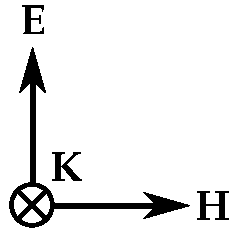
\includegraphics[width=.12\textwidth]{img/tripletEKH.pdf}}
	\end{overpic}
\end{figure}
%}}}
\begin{figure}[t] %fg_expe_fishnets %{{{
	\caption{Experimental and simulated amplitude of transmittance for fishnets \textbf{(a)} with 180$\times$200 $\mu$m holes, and \textbf{(b)} with 230x255  $\mu$m holes.  } 
		\label{fg_expe_fishnets} 
		\centering \vspace{-3mm}
\begin{tabular}{r}
\begin{overpic}[width=0.95\textwidth]{img-expe/expe_laserfishnets_t_ap.pdf} \put (-1,28) {\textbf{(a)}} \end{overpic}\vspace{-0.055\textwidth}\\
\begin{overpic}[width=0.95\textwidth]{img-expe/expe_laserfishnets_t_cp.pdf} \put (-1,28) {\textbf{(b)}} \end{overpic}\vspace{-0.055\textwidth}\\
%\begin{overpic}[width=0.95\textwidth]{img-expe/expe_laserfishnets_t_cs.pdf} \put (-1,27) {\textbf{(a)}} \end{overpic}\vspace{-0.055\textwidth}\\
%\begin{overpic}[width=0.95\textwidth]{img-expe/expe_laserfishnets_t_as.pdf} \put (-1,27) {\textbf{(a)}} \end{overpic}\vspace{-0.055\textwidth}\\
\end{tabular}
\end{figure}
%}}}
\paragraph{Experimental results} %{{{
By femtosecond laser machining of steel foils, we have fabricated series of fishnets (Fig. \ref{fg_fishnet28_photo}). 
The experimental transmittance spectra of these two samples are presented in Fig. \ref{fg_fishnet28_r}

%TODO add? Part of the fishnets were made of two foils as a metal-insulator-metal structure, but their spectra were also hard to interpret.

%Our group received another fishnet sample made by automated mechanical drilling (Fig. \ref{fg_fishnet_mechanical}) into a double-sided circuit board blank, consisting of two 30 $\upmu$m copper foils glued to a plastic. %?? material, thickness?
%The sample was measured by the terahertz spectroscopy yielding relatively complicated spectra, which could not be reasonably matched by any of the simulations. We assume that the clash between the measured and simulated values comes from the imprecision in the sample itself, namely from the burrs from drilling.
%\begin{figure}[ht]  %fg_fishnet_mechanical
	%\caption{A drilled fishnet with $500\times 500$ $\mu$m periodicity. The inclined view from the bottom side shows the burrs that were probably responsible for the large difference of the measured and simulated spectra.}  \centering 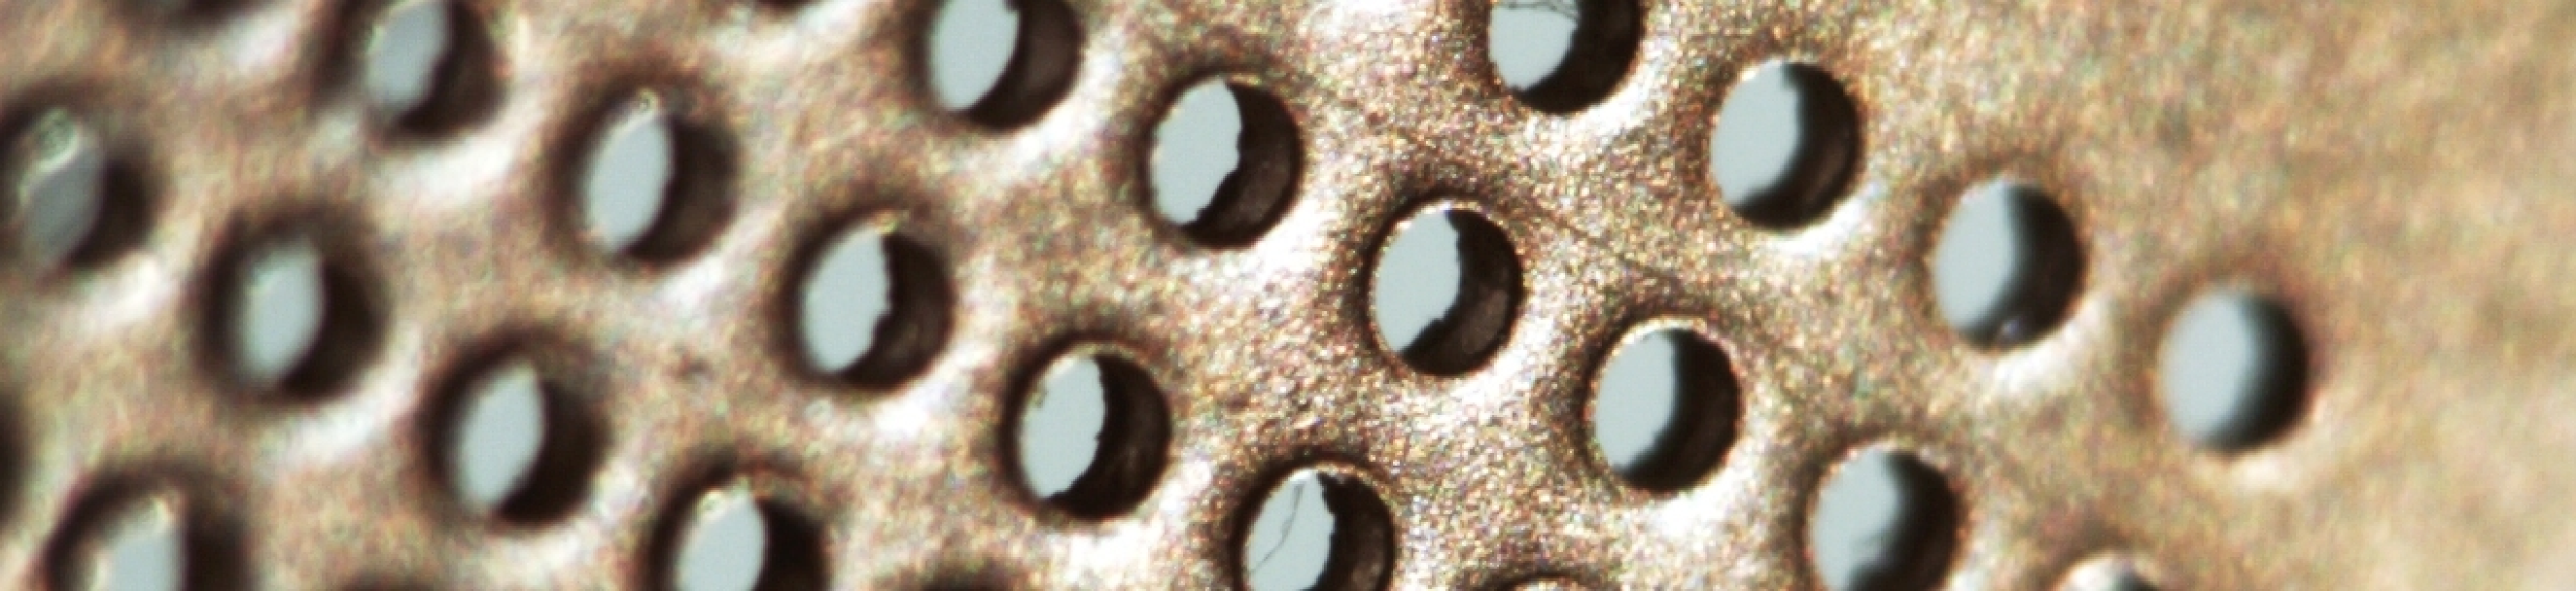
\includegraphics[width=.8\textwidth]{img/fishnet.pdf} \label{fg_fishnet_mechanical} 
%\end{figure}

%}}}
\begin{figure}[th] % fg_fnquadrup%{{{
  \begin{minipage}[b]{0.39\textwidth}
\begin{overpic}[width=.98\textwidth]{img/fishnet_quadrupole_modeE.pdf} 
\put(105,-0){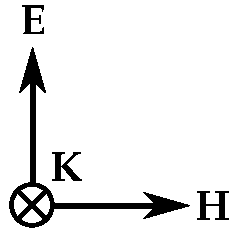
\includegraphics[width=.27\textwidth]{img/tripletEKH.pdf}}
\end{overpic}\\
  \end{minipage}
	  \vspace{1cm}
  \begin{minipage}[b]{0.6\textwidth}
	  \caption{
	  Electric field of the quadrupole mode in a fishnet with 180$\times$200 $\mu$m hole sizes. Field vectors are represented by black arrows in the $x$-$y$ plane of the fishnet; due to symmetry, the $E_z$ component in this plane is zero. The color map shows the magnitude of the $\E$ vector, the brighter values correspond to more intensive field. Surrounding light-gray structure is the metal of the fishnet.\\
  \vspace{15mm}} \label{fg_fnquadrup}
  \end{minipage}  
\end{figure} 
%}}}
\paragraph{Quadrupole resonance in experimental data}%{{{
For simulation of the fishnet, different grid resolutions were used. While usually 2 or 4 $\upmu$m voxel sizes were used throughout the thesis as a good tradeoff of simulation time and accuracy of results, in Fig.  \ref{fg_fnquadrup} the FDTD simulation was deliberately set to very coarse, with a voxel dimension of 10 $\mu$m. Still, the experimental and computed reflectance spectra yielded a very good match without any additional corrections.

In most terahertz transmittance spectra of fishnets, a relatively sharp notch between 0.5 and 1.0 THz was observed. The discretisation error has helped to explain it, since it broke the twofold mirror symmetry of the fishnet hole. 

This way, it also broke the symmetry of the first predominantly quadrupole mode, introducing a slight electric dipole into its field pattern  (see Fig. \ref{fg_fnquadrup}). As a result, the quadrupole started to coupling with the incident plane wave, and very narrow resonances emerged also in the simulated spectra in Fig. \ref{fg_expe_fishnets}, at 880 and 710 GHz, respectively. These values, still without any user intervention, the experimentally observed resonance notches close to these frequencies as a result of excitation of a quadrupole resonance.   % todo these resonances can be also observed in the CDH plots in Fig. \ref{fg_fishnet_cdh}a,b

%}}}


% pairs of rods [10], [12], [31], pair of crosses [32]
% Aleian 2012 Plasmonic Au SiO2 nanoparticles

% TODO Ye2013 Negative Group Velocity in the Absence of Absorption Resonance
 
}
